\documentclass[12pt,openright,twoside,a4paper,english,french,spanish,brazil]{abntex2}

\usepackage{cmap}	
\usepackage{lmodern}	
\usepackage[T1]{fontenc}	
\usepackage[utf8]{inputenc}		
\usepackage{lastpage}		
\usepackage{indentfirst}
\usepackage{color}	
\usepackage{graphicx}	
\usepackage{units}
\usepackage[brazilian,hyperpageref]{backref}
\usepackage[alf]{abntex2cite}
\usepackage{bold-extra}
\usepackage{eso-pic}
\usepackage{multirow}

\renewcommand{\backrefpagesname}{Citado na(s) página(s):~}
\renewcommand{\backref}{}
\renewcommand*{\backrefalt}[4]{
	\ifcase #1 %
		Nenhuma citação no texto.%
	\or
		Citado na página #2.%
	\else
		Citado #1 vezes nas páginas #2.%
	\fi}%
% ---


\usepackage{fixos/customizacoes}
\usepackage[table]{xcolor}
\usepackage{pdflscape}
\usepackage{listings}

\lstset{language=Ruby, numbers=left, numberstyle=\small} 

% Dados pessoais
\autor{Ebenezer Andrade da Silva}
\curso{Engenharia de Software}

% Dados do trabalho
\titulo{Catálogo de Segurança para o Padrão Arquitetural MVC: Modelagem Orientada a Grafos de Interdependências de Requisitos Não Funcionais}
\data{2017}
\palavraChaveUm{Palavra-chave01}
\palavraChaveDois{Palavra-chave02}

% Dados da orientacao
\orientador{Profª Dra. Milene Serrano}
\coorientador{Profº Dr. Maurício Serrano}

% Dados para a ficha catalográfica
\cdu{02:141:005.6}

% Dados da aprovação do trabalho
\dataDaAprovacao{01 de junho de 2013 -- Data da aprovação do trabalho}
\membroConvidadoUm{Titulação e Nome do Professor Convidado 01}
\membroConvidadoDois{Titulação e Nome do Professor Convidado 02}

\local{Brasília, DF}
\instituicao{%
  Universidade de Brasília -- UnB
  \par
  Faculdade UnB Gama -- FGA
}
\tipotrabalho{Trabalho de Conclusão de Curso}
\preambulo{Monografia submetida ao curso de graduação em \imprimircurso\ 
da Universidade de Brasília, como requisito parcial para obtenção do Título 
de Bacharel em \imprimircurso.}

\definecolor{blue}{RGB}{41,5,195}
\makeatletter
\hypersetup{
     	%pagebackref=true,
		pdftitle={\@title}, 
		pdfauthor={\@author},
    	pdfsubject={\imprimirpreambulo},
	    pdfcreator={LaTeX with abnTeX2},
		pdfkeywords={abnt}{latex}{abntex}{abntex2}{trabalho acadêmico}, 
		colorlinks=true,       		% false: boxed links; true: colored links
    	linkcolor=blue,          	% color of internal links
    	citecolor=blue,        		% color of links to bibliography
    	filecolor=magenta,      		% color of file links
		urlcolor=blue,
		bookmarksdepth=4
}
\makeatother
\setlength{\parindent}{1.3cm}
\setlength{\parskip}{0.2cm}  
\makeindex


\begin{document}

\frenchspacing 
\imprimircapa
\imprimirfolhaderosto*

\begin{fichacatalografica}
	\vspace*{\fill}					% Posição vertical
	\hrule							% Linha horizontal
	\begin{center}					% Minipage Centralizado
	\begin{minipage}[c]{12.5cm}		% Largura
	
	\imprimirautor
	
	\hspace{0.5cm} \imprimirtitulo  / \imprimirautor. --
	\imprimirlocal, \imprimirdata-
	
	\hspace{0.5cm} \pageref{LastPage} p. : il. (algumas color.) ; 30 cm.\\
	
	\hspace{0.5cm} \imprimirorientadorRotulo~\imprimirorientador\\
	
	\hspace{0.5cm}
	\parbox[t]{\textwidth}{\imprimirtipotrabalho~--~\imprimirinstituicao,
	\imprimirdata.}\\
	
	\hspace{0.5cm}
		1. \imprimirpalavrachaveum.
		2. \imprimirpalavrachavedois.
		I. \imprimirorientador.
		II. Universidade de Brasília.
		III. Faculdade UnB Gama.
		IV. \imprimirtitulo\\ 			
	
	\hspace{8.75cm} CDU \nomecdu\\
	
	\end{minipage}
	\end{center}
	\hrule
\end{fichacatalografica}

%%\begin{errata}
%Elemento opcional da \citeonline[4.2.1.2]{NBR14724:2011}. \textbf{Caso não 
%deseje uma errata, deixar todo este arquivo em branco}. Exemplo:

%\vspace{\onelineskip}
%
%sFERRIGNO, C. R. A. \textbf{Tratamento de neoplasias ósseas apendiculares com
%reimplantação de enxerto ósseo autólogo autoclavado associado ao plasma
%rico em plaquetas}: estudo crítico na cirurgia de preservação de membro em
%cães. 2011. 128 f. Tese (Livre-Docência) - Faculdade de Medicina Veterinária e
%Zootecnia, Universidade de São Paulo, São Paulo, 2011.

%\begin{table}[htb]
%\center
%\footnotesize
%\begin{tabular}{|p{1.4cm}|p{1cm}|p{3cm}|p{3cm}|}
%  \hline
%   \textbf{Folha} & \textbf{Linha}  & \textbf{Onde se lê}  & \textbf{Leia-se}  \\
%    \hline
%    1 & 10 & auto-conclavo & autoconclavo\\
%   \hline
%\end{tabular}
%\end{table}

%\end{errata}

\begin{folhadeaprovacao}

  \begin{center}
    {\ABNTEXchapterfont\large\imprimirautor}

    \vspace*{\fill}\vspace*{\fill}
    {\ABNTEXchapterfont\bfseries\Large\imprimirtitulo}
    \vspace*{\fill}
    
    \hspace{.45\textwidth}
    \begin{minipage}{.5\textwidth}
        \imprimirpreambulo
    \end{minipage}%
    \vspace*{\fill}
   \end{center}
    
   %Trabalho aprovado. \imprimirlocal, \imprimirdatadaaprovacao:

   \assinatura{\textbf{\imprimirorientador} \\ Orientadora} 
   \assinatura{\textbf{\imprimircoorientador} \\ Coorientador}
   \assinatura{\textbf{\imprimirmembroconvidadoum} \\ Convidado 1}
      
   \begin{center}
    \vspace*{0.5cm}
    {\large\imprimirlocal}
    \par
    {\large\imprimirdata}
    \vspace*{1cm}
  \end{center}
  
\end{folhadeaprovacao}

\begin{dedicatoria}
   \vspace*{\fill}
   \centering
   \noindent

   \textit{Esta monografia é dedicada aos meus pais, Elenira Andrade e José Elieser Filho, que\\
   me educaram, me ensinaram, e suportaram a distância e a saudade de um filho, para que esta monografia pudesse ser escrita. Em homenagem, dedico ainda essa monografia à memória de minha querida avó paterna, Maria Alicina da silva.} \vspace*{\fill}
\end{dedicatoria}

\begin{agradecimentos}

	Agradeço, primeiramente, a Deus, que sempre foi meu porto seguro e me deu forças para enfrentar e superar todas as dificuldades.
	 
	Agradeço à excelente Universidade de Brasília e ao corpo docente de graduação em Engenharia de Software, em especial aos professores, Profª. Milene Serrano e Profº. Maurício Serrano, por toda paciência e disponibilidade em me orientar; pelo suporte; pelas suas correções e incentivos, e por ensinarem conceitos de extrema importância nas áreas de Desenho de Software e Requisitos de Software; e ao Profº. George Marsicano Corrêa, por ter aberto meu horizonte sobre Requisitos de Software de uma maneira tão fantástica e exemplar.
	
	Aos meus pais, meus avós, meus irmãos, bem como ao meu cunhado, Flávio Carlos, por todo amor, incentivo e apoio durante toda minha graduação. 
	
	Aos irmãos na amizade, Jonas da Silva e Heleno da Silva, por confiarem em meu potencial, incentivando-me sempre. 
	
	Ao meu primo, Oziel da Silva, por me auxiliar nos momentos difíceis. 
	
	A meus amigos de graduação, Matheus Silva, Pedro Ivo de Andrade, Attany Araújo, Keli Cristina, Vinicius Bandeira, Maxwell Oliveira, Thiago Nunes, Yan Watanabe, João Paulo Mendonça, Hebert Douglas, Renan Costa e João Henrique, por toda ajuda com dúvidas e troca de conhecimento durante minha graduação. 
	
	Aos apoiadores, Adriana Matrins, Vick Martins, Omar Júnior, Omar Faria, Ygor Mota, Laisa Paiva, Maria Walcira, Franscico de Sousa, Rafael Paiva, Cirilo Júnior, Victor Hugo, Gabriela Nara, Luiza Lopes, Valter Avelino, Eliana e Odair,  por me acolherem nos dias difíceis longe da minha família,  e me darem apoio emocional durante minha graduação e a escrita dessa monografia. 
	
	À Milena Lima, por ser conselheira e por todo apoio emocional para que eu pudesse redigir esta monografia, acreditando em meu potencial e incentivando-me.
	
	A todos que de forma direta ou indiretamente contribuiram para realização desta monografia, e fizeram parte da minha formação. 
	
	Meu muito obrigado!  
	
\end{agradecimentos}

\begin{epigrafe}
    \vspace*{\fill}
	
		\begin{flushright}
		\textit{“Somente pensamos quando confrontados com um problema.”} \\
		\textbf{John Dewey}
		\end{flushright}
	
	
\end{epigrafe}

\begin{resumo}
 Este trabalho teve como principal objetivo a construção de um catálogo de segurança para o Padrão Arquitetural MVC (\textit{Model-View-Controller}), visando auxiliar Engenheiros de Requisitos e Engenheiros de Software na especificação dos requisitos associados ao requisito não funcional de Segurança. Utilizando modelagem orientada a grafos de interdependência de requisitos não funcionais, levando em consideração as boas práticas da Engenharia de Requisitos Orientada à Meta. Foi então, modelado na notação do NFR \textit{Framework} o Catálogo de Segurança, fundamentando-se principalmente nos conceitos de Segurança apresentados por Chung, baseando-se em Confidencialidade, Integridade e Disponibilidade, adicionalmente o catálogo apoia na definição de Segurança da Informação definida na ISO 27001. Além disso, foi aplicado ao padrão arquitetural MVC, onde verifica-se a relação das metas flexíveis e operacionalizações com as camadas do Padrão Arquitetural MVC.

 \vspace{\onelineskip}
    
 \noindent
 \textbf{Palavras-chaves}: NFR \textit{Framework}. \textit{Model-View-Controller}. Segurança de Software. Engenharia de Requisitos Orientada à Meta. Catálogo de Segurança. Padrão Arquitetural. \textit{Softgoal Interdependency Graphs}.
\end{resumo}

\begin{resumo}[Abstract]
 \begin{otherlanguage*}{english}
   The main objective of this research was the construction of a Security Catalog for the MVC (Model-View-Controller) Architectural Pattern, 
   aiming at assisting Requirements Engineers and Software Engineers in specifying the requirements associated with Security, a non-functional requirement. The catalog is documented based on a graph-oriented modeling of interdependence of non-functional requirements, taking into account good practices of Goal-Oriented Requirements Engineering. In the construction of this catalog, some pillars were considered, such as concepts associated to Security and substantiated on authors of the area, with emphasis on Confidentiality, Integrity and Availability, in addition to the definition of Information Security established by ISO 27001. As an extension of the catalog's base contributions, it has been mapped to/associated with the MVC pattern layers in order to further assist catalog users while developing their applications based on this three-tier Architectural Pattern. Lastly, the catalog has been applied in different usage scenarios, which has made possible not only a catalog with a high level of abstraction, based on the interdependencies of the non-functional requirements correlated with Security, but also a catalog that agrees a series of operations , which they seek to fulfill (at least satisfactory) with the specified non-functional requirements

   \vspace{\onelineskip}
 
   \noindent 
   \textbf{Key-words}: Software Security Catalog. Architectural Pattern Model-View-Controller. Goal-Oriented Requirements Engineering. Security. Confidentiality. Integrity. Availability. 
 \end{otherlanguage*}
\end{resumo}

\pdfbookmark[0]{\listfigurename}{lof}
\listoffigures*
\cleardoublepage
\pdfbookmark[0]{\listtablename}{lot}
\listoftables*
\cleardoublepage

\begin{siglas}
  \item[RNF] Requisito Não Funcional
  \item[MVC] \textit{Model-View-Controller}
  \item[SIGs] \textit{Softgoal Interdependecy Graphs}
  \item[i*] \textit{Framework} de modelagem i* (i-estrela)
  \item[SD] \textit{Strategic Dependency}
  \item[SR] \textit{Strategic Rationale}
  \item[ISO] \textit{International Organization of Standardization}
  \item[IEC] \textit{International Electrotechnical Commission}
  \item[UML] \textit{Unified Modeling Language}
  \item[FURPS] \textit{Functionality, Usability, Reliability, Performance, Supportability}
  \item[MTBF] \textit{Mean Time Between Failure}
  \item[NBR] Norma Brasileira
  \item[ABNT] Associação Brasileira de Normas Técnicas
  \item[GUI] \textit{Graphical User Interface}
  \item[ERD] \textit{Entity Relationship Diagram}
  \item[DFD] \textit{Data Flow Diagram}
  \item[MDA] \textit{Model Driven Architecture}
  \item[RE-Tools] \textit{Requirements Engineering - Tools}
  \item[BPMN] \textit{Business Process Model and Notation}
  \item[CIA] \textit{Confidenciality, Integrity, Availability}
  \item[TCC] Trabalho de Conclusão de Curso
  \item[GORE] \textit{Goal-Oriented Requirements Engineering}
  \item[KAOS] \textit{Knowledge Acquisition in autOmated Specification}
  \item[URL] \textit{Uniform Resource Locator}
  \item[RoR] \textit{Ruby on Rails}
  \item[SGBD] Sistema de Gerenciamento de Banco de Dados
  \item[GPL] \textit{General Public License}
  \item[HTML] \textit{HyperText Markup Language}
  \item[CSS] \textit{Cascading Style Sheets}
  \item[QR] \textit{Quick Response}
\end{siglas}

%%\begin{simbolos}
%  \item[$ \Gamma $] Letra grega Gama
%  \item[$ \Lambda $] Lambda
%  \item[$ \zeta $] Letra grega minúscula zeta
%  \item[$ \in $] Pertence
%\end{simbolos}

\pdfbookmark[0]{\contentsname}{toc}
\tableofcontents*
\cleardoublepage



\textual

\chapter{Introdução}
\label{chap:introducao}

Neste capítulo, são descritos o contexto, no qual o trabalho está inserido; a questão de pesquisa, a qual norteia o embasamento científico do trabalho;  a justificativa, visando destacar a contribuição dessa pesquisa; os objetivos geral e específicos, com os quais são acordadas as principais metas a serem atingidas para conclusão do trabalho, e por fim, a organização dos demais capítulos dessa monografia.

\section{Contextualização}

Os requisitos não-funcionais (RNFs) e funcionais descrevem as características de um software, focando nas questões: \textbf{como esse software deve fazer?} e \textbf{o que esse software deve fazer?}  \cite{sommerville1997requirements}. Frequentemente, os RNFs são especificados de forma equivocada ou ainda são negligenciados, não sendo especificados \cite{eckhardt2016non}. Visando auxiliar os Engenheiros de Requisitos na tarefa de especificar os RNFs, os autores, em \cite{mairiza2010investigation}, destacam 114 classes de RNFs. Dentre essas classes, as mais mencionadas na literatura são: 1º Desempenho, 2º Confiabilidade e  3º Usabilidade. No contexto empresarial, ou seja, mais aplicado e comercial, as classes de RNFs mais utilizadas nas especificações são: 1º Segurança, 2º Confiabilidade e 3º Usabilidade \cite{eckhardt2016non}. Como o foco desse trabalho é atuar especificamente em suporte aplicáveis no contexto empresarial, pretende-se contribuir com a especificação do RNF de segurança, dado que é a classe de RNF mais relevante para o mercado, de acordo com a literatura investigada.

Ao desenvolver um software, os RNFs impactam, segundo \cite{eckhardt2016non}, na implementação, manutenção, operacionalização e utilização de recursos. Adicionalmente, impactam em aspectos arquiteturais de uma aplicação de software, sendo necessário especificar a arquitetura orientando-se não apenas pelos requisitos funcionais, mas também pelos RNFs \cite{buschmann1996system}

Dependendo do padrão arquitetural utilizado, as especificações bem como as operacionalizações dos RNFs podem variar \cite{chung2012non}. Diante do exposto, e visando focar em um padrão arquitetural comumente utilizado, o presente trabalho pretende orientar-se pelo padrão arquitetural \textit{Model-View-Controller} (MVC). Trata-se de um padrão bem aceito, bem como utilizado no desenvolvimento de aplicações Web, sendo inclusive base para o desenvolvimento dessas aplicações em \textit{frameworks} e plataformas de geração de código mais emergentes, orientadas à Convenção sobre Configuração \cite{jailia2016behavior}.


O MVC é um padrão arquitetural para sistemas interativos, que divide a aplicação em componentes: a \textit{Model}, que contém a implementação das funcionalidades principais e os dados da aplicação, ou seja as entidades de domínio; a \textit{View}, que exibe as informações da aplicação ao usuário, sendo, portanto, a camada mais próxima desse último, e a \textit{Controller}, que lida com as entradas do usuário \cite{buschmann1996system}, sendo um componente intermediário entre \textit{Model} e \textit{View}.  

Existem alguns \textit{frameworks} conceituais centrados na especificação de RNFs. Dentre eles, destacam-se: NFR Framework \cite{chung2009non}, i* \cite{istarwiki20} e FURPS \cite{umar2011analyzing}. Detalhes sobre esses frameworks serão cobertos no Capítulo \ref{chap:referencialTeorico} dessa monografia, Referencial Teórico. Em um primeiro momento, pode-se destacar que os dois primeiros, NFR Framework e i*, fazem uso de uma abordagem mais emergente para especificação desses RNFs. Já o FURPS pode ser entendido como um documento simples, especificado em linguagem natural, que se orienta por alguns RNFs comumente encontrados na literatura, no caso (em inglês): \textit{Functionality}, \textit{Usability}, \textit{Reliability}, \textit{Performance} e \textit{Supportability}.

A abordagem mais emergente, mencionada para os \textit{frameworks} NFR e i*, usa modelos específicos, focados na especificação de requisitos usando princípios da \textit{Goal-Oriented Requirements Engineering} (GORE) \cite{horkoff2016goal}. Rastreabilidade de requisitos \cite{wiegers2013software}; especificação de impactos e interdependências entre os requisitos; registro de alternativas quanto aos requisitos analisados, e definição de operacionalizações para viabilizar a realização dos requisitos são algumas vantagens que ficam evidentes no uso desses modelos mais específicos, como, por exemplo: o \textit{Softgoal Interdependency Graphs} (SIGs) \cite{chung2012non} ou, em português, Grafos de Interdependências entre Requisitos Não Funcionais. 

Portanto, esse trabalho propôs a definição de um Catálogo de SIGs centrado no RNF Segurança, especificamente desenhado para o Padrão Arquitetural MVC, usando a notação do NFR Framework. Com a intenção de auxiliar os Engenheiros de Requisitos e ainda os Engenheiros de Software na tarefa de especificação de requisitos não funcionais e funcionais quando uma arquitetura for imposta. Como o catálogo ficaria muito abrangente e generalista, caso fosse definido para qualquer RNF e padrão arquitetural, não sendo, portanto, útil, focou-se: (i) no RNF mais preocupante - Segurança, segundo a literatura - em aplicações de software de cunho comercial; (ii) em aplicações Web, e (iii) no padrão arquitetural MVC.  Vale ressaltar ainda que os termos RNFs, atributos de qualidade, critérios de qualidade e metas flexíveis serão utilizados como sinônimos ao longo dessa monografia.


\section{Questão de Pesquisa}
Este trabalho procurou responder a seguinte questão de pesquisa: \textit{Como auxiliar Engenheiros de Requisitos e Engenheiros de Software na especificação de RNFs quando uma arquitetura é imposta?} É relevante comentar que essa resposta ao final do trabalho, pareceu parcial, pois o trabalho exemplificou esse auxílio usando como base o RNF Segurança, aplicações Web e o padrão arquitetural MVC. Entretanto, cabe ao  ao leitor extrapolar as particularidades desse exemplo, usando-o como base mesmo quando outro RNF for foco bem como outro padrão arquitetural for imposto.

É recomendado que uma questão de pesquisa seja organizada em três visões \cite{keele2007guidelines}: 
\textbf{População}, estabelecendo quem são as pessoas diretamente afetadas pela intervenção; \textbf{Intervenção}, comparando dois ou mais "tratamentos alternativos", ou seja, duas ou mais possíveis estratégias de atuação, e \textbf{Saídas}, estabelecendo a forma como a intervenção vem sendo aplicada. Nesse contexto, tem-se: 

\begin{itemize}
	\item População: "\textit{..Engenheiros de Requisitos e Engenheiros de Software na especificação de requisitos associados ao RNF Segurança, em aplicações Web desenvolvidas orientando-se pelo padrão arquitetural MVC..}"
	\item Intervenção: "\textit{..utilização de notação específica, NFR Framework, para modelagem dos Grafos de Interdependências de Requisitos Não Funcionais centrados no critério de qualidade Segurança, especificando impactos, interdependências e operacionalizações cabíveis  ..}"
	\item Saídas: "\textit{.. catálogo de soluções centrado em Segurança e no padrão arquitetural MVC..}"
\end{itemize}
\section{Justificativa}


Observou-se que mesmo com uma \textit{baseline}  arquitetural definida, os RNFs, chamados também de atributos ou critérios de qualidade, são negligenciados ou tratados de forma equivocada \cite{eckhardt2016non}. Entretanto, esses critérios evidenciam preocupações, as quais impactam na qualidade do software em desenvolvimento \cite{schneidewind1990standard}.  
Portanto, são necessários esforços para auxiliar os Engenheiros de Requisitos e os Engenheiros de Software na especificação desses RNFs, em particular em aplicações tipicamente comerciais, cujas arquiteturas são, normalmente, impostas pelas empresas de desenvolvimento.

Nesse trabalho então definiu um catálogo de SIGs centrado no RNF Segurança, no escopo das aplicações web, e no padrão arquitetural MVC aplicado em cenários de desenvolvimento onde a tecnologia utilizada foi \textit{rails} que trata-se de um framework de desenvolvimento web baseado no padrão arquitetural MVC. 

\section{Objetivos}
 
\subsection{Objetivo Geral}

Definir catálogo de segurança para o padrão arquitetural MVC usando modelagem orientada a grafos de interdependências de RNFs, ou seja, levando em consideração as boas práticas acordadas na Engenharia de Requisitos Orientada à Meta (em inglês, \textit{Goal Oriented Requirements Engineering} - GORE). 

\subsection{Objetivos Específicos}

Com intuito de alcançar o objetivo geral, foram considerados relevantes os seguintes objetivos específicos:

\begin{itemize}
	
	\item Investigar - na literatura: (i) formas recomendadas para lidar com o RNF Segurança em aplicações web desenvolvidas com base no padrão arquitetural MVC, permitindo identificar alternativas e operacionalizações para concretização desse RNF de forma satisfatória, e (ii) RNFs associados à Segurança, permitindo identificar as interdependências e os impactos entre eles;
	
	\item Elaborar o catálogo de SIGs, com base nos resultados da etapa de investigação (supracitada) bem como orientando-se pela notação do NFR Framework;
	
	\item Realizar a correspondência entre o  catálogo e as camadas do padrão arquitetural MVC;
	
	
	\item Elaborar cenários e desenvolver aplicações web exemplo, no padrão MVC, orientando-se pelo catálogo. Essas aplicações web exemplo podem ser vistas como cenários de uso ou um estudo de caso, procurando apresentar aos interessados como o catálogo pode ser utilizado/instanciado. 
	
\end{itemize}

\section{Organização da Monografia}

Esta monografia está dividida nos respectivos capítulos, sendo eles: 
\begin{itemize}
	\item O Capítulo \ref{chap:referencialTeorico} \textbf{Referencial Teórico}, explora os conceitos chave para elaboração da monografia, partindo da engenharia de requisitos e seus conceitos, explora-se também os aspectos e conceitos de arquitetura de software e o padrão MVC, bem como a visão dos requisitos de segurança como RNFs;
	
	\item  O Capítulo \ref{chap:suporteTecnologico} \textbf{Suporte Tecnológico}, apresenta as ferramentas de modelagem dos diagramas e mapas mentais, e as ferramentas de suporte à escrita utilizadas para o desenvolvimento da monografia;
	
	\item O Capítulo \ref{chap:metodologia} \textbf{Metodologia}, enfoca as questões da classificação da pesquisa e os procedimentos metodológicos para o desenvolvimento dessa monografia;
	
	\item O Capítulo \ref{chap:proposta} \textbf{Proposta}, descreve o catálogo de tipos de RNFs para segurança e o gráfico de interdependência entre as metas flexíveis (SIGs);
	
	\item  O Capítulo \ref{chap:consideracoesFinais} \textbf{Considerações Finais}, apresenta os resultados alcançados com a execução do TCC1 e o que espera alcançar com a execução do TCC2.
\end{itemize}


\chapter[Referencial Teórico]{Referencial Teórico}
\label{chap:referencialTeorico}

Neste capítulo, serão apresentados os conceitos teóricos utilizados como base para o desenvolvimento do catálogo de segurança para o padrão arquitetural MVC.

Antes de entender os conceitos relevantes para o desenvolvimento do catálogo, é importante entender a definição de software. Este, segundo \cite{sommerville2003engenharia}, pode ser entendido como programas de computador e toda documentação associada. Para realização do desenvolvimento do software da forma mais correta possível, existem preocupações que merecem menção/atenção e são estabelecidas na área da Engenharia de Software que preocupa-se com todos os aspectos da produção \cite{sommerville2003engenharia}. 

A Figura \ref{BigPicture} apresenta o escopo de atuação desse trabalho, partindo da Engenharia de Software e apoiando-se, principalmente em duas disciplinas: 

\begin{itemize}
	
	\item A Engenharia de Requisitos, que se compõe de um conjunto de tarefas e técnicas que auxiliam a promoção do entendimento dos requisitos, sendo uma disciplina detalhada na seção \ref{sec:requisitos}. Será observado que o trabalho foca em uma abordagem orientada à meta. Portanto, tem-se a Engenharia de Requisitos Orientada à Meta. Essa procura tratar os requisitos funcionais e não funcionais como metas a serem alcançadas, sendo esse estudo apresentado na subseção \ref{subsec:orientacaoMeta}. Especificando ainda mais a área de atuação, como esse trabalho centraliza seus esforços nos RNFs, em particular para elaboração do catálogo, a subseção \ref{subsec:requisitosNaoFuncionais} define conceitos associados aos RNFs, preparando o leitor para a apresentação de um \textit{framework} conceitual especificamente proposto para especificação de RNFs. Trata-se do NFR Framework, o qual será detalhado na seção \ref{sec:NFR};
	
	\item E Desenho de Software, uma área da Engenharia de Software que se preocupa, dentre outras atividades, com o planejamento e a definição da Arquitetura de Software a ser utilizada. Para fins desse trabalho, o foco será na arquitetura padrão MVC. Conceitos associados à Arquitetura de Software bem como ao padrão arquitetural MVC serão detalhados na seção \ref{sec:arquitetura} e não subseção \ref{subsec:mvc}, respectivamente.
	
\end{itemize}

\pagebreak

\begin{figure}[h!]
	\centering
	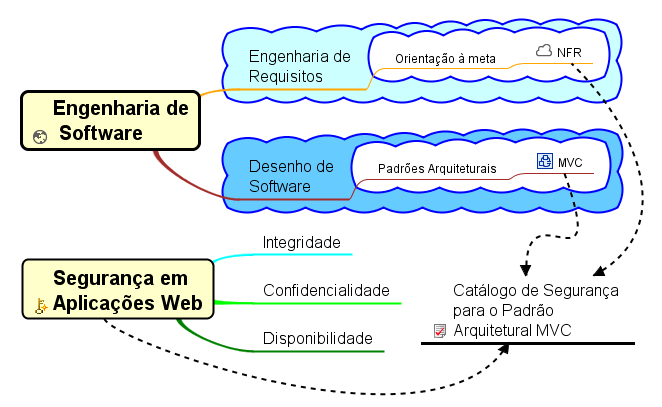
\includegraphics[keepaspectratio=true,scale=0.8]{figuras/bigPicture.png}
	\caption{Áreas de atuação  da presente proposta e conceitos associados.}
	\label{BigPicture}
\end{figure}

Por fim, cabe ressaltar que o presente trabalho atuará mais especificamente no requisito não funcional segurança, dada a sua relevância, conforme pesquisa na literatura. Segundo \cite{chung2012non}, segurança pode ser entendida como a satisfação de três conceitos: Integridade, Confidencialidade, e Disponibilidade. Portanto, o catálogo de segurança proposto parte desses conceitos, seguindo a expressão \ref{eq:EstruturaLogicaDeSeguranca}. Segurança, sobre a ótica de um RNF, será tratada na seção \ref{sec:seguranca}.

\begin{equation}
	\label{eq:EstruturaLogicaDeSeguranca}
	\textrm{Integridade E Confidencialidade E Disponibilidade SATISFAZ Segurança}
\end{equation}

\section{Engenharia de Requisitos}
\label{sec:requisitos}

Ao conjunto de tarefas e técnicas utilizadas para promover o entendimento dos requisitos é denominado Engenharia de Requisitos \cite{pressman2011engenharia}. No desenvolvimento de software, ela pode ser vista como uma fase importante da Engenharia de Software, que se inicia nas atividades de comunicação com os \textit{stakeholders}, e continua até a entrega do produto, sendo adaptada de acordo com as necessidades do processo de desenvolvimento, do produto e dos \textit{stakeholders} \cite{pressman2011engenharia}.

A Engenharia de Requisitos abrange sete fases distintas: concepção, levantamento, elaboração, negociação, especificação, verificação e validação \cite{pressman2011engenharia}. De acordo com \cite{kotonya1998requirements}, durante a execução das atividades nas fases da Engenharia de Requisitos, alguns problemas são relatados como: (i) os requisitos não refletem as reais necessidades do cliente, de acordo com o sistema a ser desenvolvido; (ii) os requisitos são inconsistentes e/ou incompletos; (iii) a Engenharia de Requisitos é complexa e possui alto custo, principalmente, quando há necessidade de mudanças após os requisitos serem ditos acordados/elicitados entre as partes; e (iv) os requisitos são comumente interpretados de maneira errada pela equipe de desenvolvimento, diante do que foi solicitado pelo cliente. 

Boa parte dos modelos utilizados na Engenharia de Requisitos não possuem tratamento adequado para lidar com os critérios de qualidade. Logo, o tratamento desses critérios tem sido uma preocupação para a comunidade da Engenharia de Requisitos. Atualmente, existem esforços no sentido de aprimorar os modelos e especificações desses requisitos, e são fortemente associados à comunidade de pesquisadores da Engenharia de Requisitos Orientada à Meta (GORE) \cite{chung2012non}. Nesta monografia, é abordado o uso de uma notação específica para tratar RNFs, proposta por essa comunidade, no caso, trata-se do NFR \textit{framework} \cite{chung2012non}. 

O NFR \textit{framework} é um \textit{Framework} conceitual que procura lidar com os requisitos não funcionais, permitindo especificar os mesmos em um alto nível de abstração e, gradualmente, fornecendo insumos para que essa especificação seja trazida para um nível mais baixo de abstração. Nesse último nível, são especificadas as operacionalizações, as quais evidenciam alternativas para viabilizar a implementação desses requisitos no nível de código. Mais adiante, serão apresentados detalhes dessa notação.

\subsection{Engenharia de Requisitos Orientada à Meta}
\label{subsec:orientacaoMeta}

A Engenharia de Requisitos Orientada à Meta (GORE) tem-se popularizado nos últimos anos e foca seus esforços no tratamento dos requisitos funcionais e não funcionais, como metas a serem alcançadas \cite{van2001goal}, Seus modelos possuem como objetivo a modelagem da razão pela qual determinado requisito existe. Essa modelagem promove ao engenheiro de requisitos uma estratégia mais detalhada do problema, podendo encontrar uma solução mais adequada \cite{van2001goal}\cite{chung2012non}. O GORE é uma abordagem cada vez mais reconhecida na comunidade de Engenharia de Requisitos \cite{van2001goal}.

Nas definições do GORE, existem as metas que são componentes essenciais. De acordo com \cite{van2001goal}, uma meta é definida como uma propriedade do sistema, a qual é expressa pelos \textit{stakeholders} através de determinadas questões como, através de determinadas questões como, o “\textbf{porquê}” uma meta é exigida, “\textbf{como}” ela pode ser atingida, e “\textbf{quem}” será o responsável pela meta no sistema e no ambiente.

\begin{figure}[h!]
	\centering
	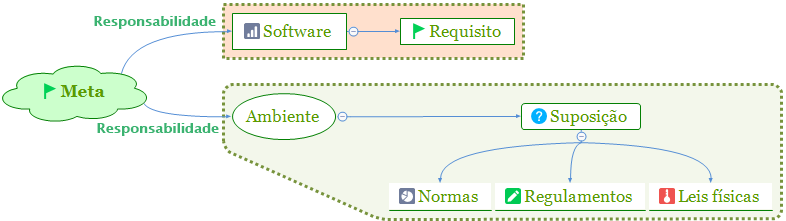
\includegraphics[keepaspectratio=true,scale=0.8]{figuras/GORE.png}
	\caption{Responsabilidades da meta sob o software e sob o ambiente.}
	\label{Gore}
\end{figure}


\pagebreak

 Com base na Figura \ref{Gore}, pode-se entender como são os comportamentos das metas na abordagem GORE. Representada pelo simbolo de uma nuvem, uma meta, quando está sob a responsabilidade de um único software, pode se tornar um requisito. De forma semelhante, quando uma meta está sob a responsabilidade de um ambiente, ela pode se tornar uma suposição. Diferentemente de um requisito, uma suposição não pode ser aplicada pelo software. Mas, pode ser satisfeita devidos às normas, aos regulamentos organizacionais e às leis físicas\cite{van2001goal}. Esse trabalho foca apenas nas responsabilidades voltadas ao software.


Existem diversos \textit{frameworks} orientados à meta. Os principais  são o NFR \textit{Framework} \cite{chung2012non} e o i* \cite{istarwiki20}. Ambos esses \textit{frameworks} serão detalhados nas seções \ref{sec:NFR} e \ref{sec:i*}, respectivamente.

\subsection{Requisitos Não-Funcionais}
\label{subsec:requisitosNaoFuncionais}

A visão do software como um produto fez com que os aspectos que avaliam a qualidade de um software passassem a possuir maior atenção. Apenas satisfazer requisitos funcionais não é o suficiente. Logo, tem-se dado maior atenção para o RNFs, tais como: Segurança, Integridade, Disponibilidade, dentre outros \cite{cysneiros1997definindo}.

Os RNFs podem ser entendidos como restrições sobre como os requisitos funcionais devem ser implementados, e determinam como o software deve realizar suas funções \cite{sommerville1997requirements}.


Júlio Leite, afirma em sua pesquisa que os RNFs impactam o produto software em qualidade e preço, pois segundo ele:

\begin{citacao}
	"A não observância da necessidade de RNFs durante o processo de desenvolvimento do software, pode levar uma recodificação custosa e demorada o que consequentemente, eleva o preço do software." \cite[p. 2]{cysneiros1997definindo}
\end{citacao}

Os RNFs devem ser analisados em toda sua magnitude para o desenvolvimento e a manutenção de um produto de software, sendo importante analisar os possíveis conflitos que podem ser gerados com outros RNFs bem como com os requisitos funcionais. Esses conflitos, uma vez não identificados em uma fase inicial do processo de desenvolvimento de software, podem acarretar em problemas futuros, durante as atividades de implementação e implantação do software \cite{cysneiros1997definindo}. 


As classes de NFRs \cite{eckhardt2016non} podem ser compreendidas como subtipos dos atributos de qualidade da Tabela \ref{AtributosDeQualidade}, na qual são definidos de acordo com a \cite{organizacion2011iso}. 

\begin{table}[h!]
	\centering
	\caption{Descrição dos atributos de qualidade. Fonte: \cite{organizacion2011iso}.}
	\label{AtributosDeQualidade}
	\begin{tabular}{@{}cc@{}}
		\toprule
		\textbf{\begin{tabular}[c]{@{}c@{}}Atributos de \\ qualidade\end{tabular}} & \textbf{Descrição} \\ \midrule
		Funcionalidade & \begin{tabular}[c]{@{}c@{}}É a capacidade do software de promover funções que\\ atendam às necessidades explícitas e implícitas.\end{tabular} \\
		\rowcolor[HTML]{C0C0C0} 
		Segurança & \begin{tabular}[c]{@{}c@{}}É a capacidade do software de apresentar níveis\\  aceitáveis e riscos de danos a pessoas, negócios\\  software, propriedades ou ambiente.\end{tabular} \\
		Confiabilidade & \begin{tabular}[c]{@{}c@{}}É a capacidade do software de manter o nível de\\ desempenho especificado.\end{tabular} \\
		\rowcolor[HTML]{C0C0C0} 
		Usabilidade & \begin{tabular}[c]{@{}c@{}}É a capacidade do software de ser compreendido,\\ de fácil aprendizagem, operável e atraente ao usuário.\end{tabular} \\
		Eficiência & \begin{tabular}[c]{@{}c@{}}É a capacidade software de apresentar desempenho\\ apropriado, relativo aos recursos utilizados.\end{tabular} \\
		\rowcolor[HTML]{C0C0C0} 
		Portabilidade & \begin{tabular}[c]{@{}c@{}}É a capacidade software de ser transferido de\\ um ambiente para o outro.\end{tabular} \\
		Manutenção & \begin{tabular}[c]{@{}c@{}}É a capacidade do software de modificado de forma\\ eficiente e eficaz.\end{tabular} \\ \bottomrule
	\end{tabular}
\end{table}

\section{NFR Framework}
\label{sec:NFR}

O NFR \textit{Framework}  é um modelo intencional, criado para ajudar engenheiros de software e engenheiros de requisitos a lidarem com requisitos não-funcionais, através de um grafo chamado de \textit{Softgoal Interdependency Graphs} (SIGs). Neste tipo de grafo, os requisitos podem ser analisados, uma vez que o SIG permite uma visão vertical desde a estratégia de alto nível até os detalhes operacionais;  possuindo operadores lógicos AND (E) e OR (OU) que promovem uma melhor tomada de decisão. Os RNFs são escritos através de uma notação formal. Essa notação permite comprovar a precisão e a completude de cada NFR \cite{chung2012non}. 

O \textit{framework} também pode ser orientado por processo, dando suporte às atividades e fases do processo de engenharia de requisitos. Nesse caso, sendo utilizado como complemento nas abordagens de desenvolvimento de software \cite{chung2012non}.

O NFR \textit{Framework} utiliza o conceito de metas  flexíveis. Por definição, uma meta flexível é uma condição ou um estado no mundo real que deseja ser alcançado, podendo assumir natureza subjetiva, uma vez que o RNF pode variar de acordo com o julgamento de cada pessoa; e natureza relativa, uma vez que o RNF pode depender de algum tipo de relação com outro RNF \cite{chung2012non}.

A notação no SIG para a \textbf{meta flexível} é um símbolo similar ao de uma nuvem, conforme apresentado pela Figura \ref{fig01}. Esse simbolo possui pequenas variações na forma, podendo representar uma \textbf{operacionalização} (nuvem em negrito), e também uma \textbf{reivindicação} (nuvem tracejada). Mais adiante, na Figura \ref{exemploNFR}, é apresentada a decomposição de uma meta flexível em outras metas.  

\begin{figure}[h!]
	\centering
	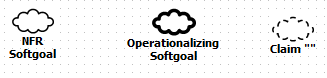
\includegraphics[keepaspectratio=true,scale=0.9]{figuras/tiposDeSoftgoals.png}
	\caption{Representação gráfica dos tipos de metas flexíveis.}
	\label{fig01}
\end{figure} 

Para facilitar no entendimento das decisões tomadas, a meta flexível possui \textit{labels}, que determinam o grau de satisfação para uma meta flexível, de acordo com um conjunto de decisões do projeto. As \textit{labels} são: satisfeita, fracamente satisfeita,  negada, fracamente negada, indecidida e crítica \cite{chung2012non}. Outra notação importante, e que apresenta o grau de prioridade de uma meta flexível, é representada por “\textbf{!}” ou “\textbf{!!}” para um grau de prioridade maior, onde o ponto de afirmação é desenhado à esquerda da nuvem.

\begin{figure}[h]
	\centering
	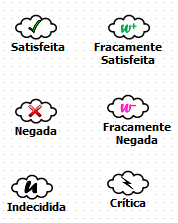
\includegraphics[keepaspectratio=true,scale=0.9]{figuras/labelsSoftgoals.png}
	\caption{Representação gráfica das \textit{labels} em metas flexíveis.}
	\label{fig02}
\end{figure} 

As relações que as metas flexíveis possuem umas com as outras são estabelecidas através de \textit{links} de interdependências, sendo esses \textit{links} que realizam o registro da decomposição das metas flexíveis em metas flexíveis mais específicas (filhos). De certa forma, a decomposição em outras metas contribui para o nível de satisfação da meta flexível mais genérica (pai).

Os \textit{links} de interdependências também podem ser entendidos como tipos de contribuições, e possuem uma notação simbólica para cada tipo, e cada tipo possui ainda um significado.  Tais tipos de contribuição são apresentados na Tabela \ref{tiposDeContribuições} adaptado de  \cite{chung2012non}.



\begin{table}[h!]
	\centering
	\caption{Tipos de contribuições.}
	\label{tiposDeContribuições}
	\begin{tabular}{@{}cl@{}}
		\hline
		\textbf{Símbolo} & \textbf{Descrição} \\ \hline
		\multirow{2}{*}{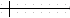
\includegraphics[scale=0.9]{figuras/And.png}} & \multirow{2}{*}{AND: Se todos os filhos são satisfeitos, o pai também será satisfeito.} \\
		&  \\ \hline
		\multirow{2}{*}{\includegraphics[scale=0.9]{figuras/OR.png}} & \multirow{2}{*}{OR: Se qualquer filho é satisfeito, o pai também será satisfeito.} \\
		&  \\ \hline
		\multirow{2}{*}{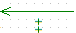
\includegraphics[scale=0.9]{figuras/Make.png}} & \multirow{2}{*}{\begin{tabular}[c]{@{}l@{}}MAKE: Pode ser tratado de forma semelhante ao AND, pois, se \\ o filho for satisfeito, o pai pode ser satisfeito.\end{tabular}} \\
		&  \\ \hline
		\multirow{2}{*}{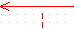
\includegraphics[scale=0.9]{figuras/Break.png}} & \multirow{2}{*}{\begin{tabular}[c]{@{}l@{}}BREAK: Fornece apoio negativo, pois, se o filho é satisfeito, o \\ pai pode ser negado.\end{tabular}} \\
		&  \\ \hline
		\multirow{2}{*}{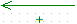
\includegraphics[scale=0.9]{figuras/Help.png}} & \multirow{2}{*}{HELP: Se todos os filhos são satisfeitos, o pai também será satisfeito.} \\
		&  \\ \hline
		\multirow{2}{*}{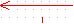
\includegraphics[scale=0.9]{figuras/Hurt.png}} & \multirow{2}{*}{HURT: Se todos os filhos são satisfeitos, o pai será fracamente negado.} \\
		&  \\ \hline
		\multirow{2}{*}{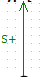
\includegraphics[scale=0.9]{figuras/SomeMais.png}} & \multirow{2}{*}{SOME+: Representa a existência de alguma contribuição positiva.} \\
		&  \\ \hline
		\multirow{2}{*}{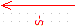
\includegraphics[scale=0.9]{figuras/SomeMenos.png}} & \multirow{2}{*}{SOME-: Representa a existência de alguma contribuição negativa.} \\
		&  \\ \hline
	\end{tabular}
\end{table}

\pagebreak

Os \textit{links} entre as metas flexíveis representam a contribuição que uma meta flexível tem com outra meta flexível, ou meta flexível de operacionalização, ou meta flexível de reivindicação. Logo, a Figura \ref{catalogoDeAvaliação} apresenta a forma como as \textit{labels} são propagadas, de acordo com seu tipo de relacionamento. A propagação das \textit{labels} aplica-se a todos os tipos de metas flexíveis. 

\begin{figure}[h!]
	\centering
	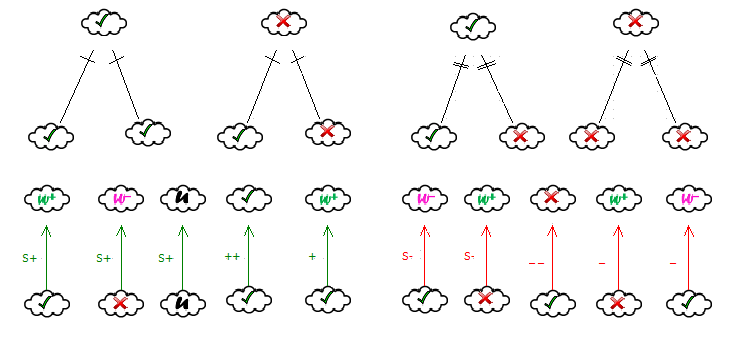
\includegraphics[keepaspectratio=true,scale=0.8]{figuras/catalogoDeAvaliacao.png}
	\caption{Propagação das \textit{labels} para os diferentes tipos de contribuição. Adaptado de \cite{chung2012non}.}
	\label{catalogoDeAvaliação}
\end{figure} 

\pagebreak

A Figura \ref{exemploNFR} apresenta uma decomposição de uma meta flexível em outras metas de mesma natureza. Consideramos, nesse exemplo, o RNF: “manter as contas com boa segurança”. Usando a notação do NFR \textit{Framework}, representou-se a meta flexível  “segurança de contas”, no nível mais generalista do grafo. Em segundo nível, são especificadas as principais metas flexíveis que merecem ser consideradas para que a meta generalista seja "satisfeita", no caso: “Integridade de contas”, “Confidencialidade de contas” e “Disponibilidade de contas” \cite{chung2012non}.

\begin{figure}[h!]
	\centering
	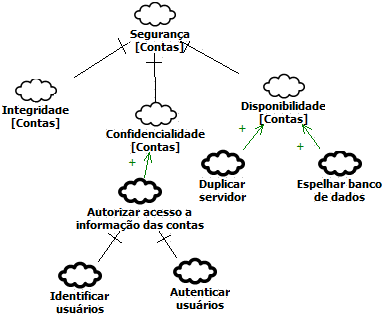
\includegraphics[keepaspectratio=true,scale=1.0]{figuras/exemploNFR.png}
	\caption{Operacionalização de segurança de contas. Adapatado de \cite{chung2012non}, \cite{affleck2012supporting}.}
	\label{exemploNFR}
\end{figure} 

Confidencialidade de contas é operacionalizada em ``Autorizar acesso à informação das contas``, que possui uma contribuição do tipo HELP com seu pai. Dada a relação do tipo AND, entre essa operacionalização e as operacionalizações ``Identificar usuários`` e ``Autenticar usuários``, tem-se que a operacionalização ``Autorizar acesso à informação das contas``  será realizada, se ambas as operacionalizações, ``Identificar usuários`` e ``Autenticar usuários``, forem realizadas. Supondo que tudo tenha sido realizado com sucesso, tem-se que esse processo de operacionalização contribui positivamente - HELP (AJUDA) - a atingir ``Confiabilidade de contas``. Como essa meta flexível está especificada em uma relação de AND com as metas flexíveis "Integridade de contas" e ``Disponibilidade de contas``, pode-se dizer que em termos de ``Confiabilidade de contas``, ``Segurança de contas`` tende a ser ``satisfeita``. Mas, resta ainda ponderar se "Integridade de contas" e ``Disponibilidade de contas`` serão de fato ``satisfeitas``. O modelo, da forma como está especificado, não permite avaliar tais aspectos, visto que representa apenas uma visão parcial dessas metas flexíveis.


Para Disponibilidade de contas, a mesma é operacionalizada em “Duplicar servidor” e “Espelhar banco de dados”. Essas operacionalizações possuem contribuições do tipo HELP e mesmo pai. Para a meta flexível ser satisfeita, ambas as operacionalizações devem ser satisfeitas \cite{affleck2012supporting}. 


\section{Framework i*}
\label{sec:i*}


Outra abordagem orientada à meta, o \textit{framework} de modelagem i*\footnote[1]{O nome i* faz referência a utilização da notação de distribuição intencional que é a base do \textit{framework}.}, possui foco em ambientes organizacionais e seus sistemas de informação, tomando como base os relacionamentos de dependência entre os atores participantes \cite{yu1997towards} \cite{istarwiki20}. 

O \textit{framework} é composto por dois modelos: o (i) Modelo de Dependência Estratégica (do inglês, \textit{Strategic Dependency - (SD)}), utilizado para descrever as relações de dependência entre vários atores em um contexto organizacional, e o (ii) Modelo de Razão estratégica (do inglês, \textit{Strategic Rationale - (SR)}), utilizado para descrever os interesses e preocupações das partes interessadas, e como eles podem ser abordados pelas configurações do ambiente e dos sistemas \cite{yu1997towards}. Esses dois modelos serão detalhados a seguir, nas subseções \ref{subsec:SD} e \ref{subsec:SR}.

Com a utilização do \textit{framework}, é possível representar, por meio de seus modelos, os atores participantes e suas dependências, para que suas metas sejam alcançadas, recursos fornecidos, tarefas realizadas e metas flexíveis sejam “satisfeitas a contento” ou “razoavelmente satisfeitas” \cite{istarwiki20}.
 
 
\subsection{Modelo de Dependência Estratégica - SD}
\label{subsec:SD}

O modelo SD é utilizado para expressar, através de uma rede de relacionamentos estratégicos e intencionais, a relação entre os atores em um contexto organizacional. Em sua modelagem, o modelo utiliza um conjunto de nós e ligações. Cada nó representa um ator, e cada ligação entre dois atores indica que um determinado ator depende de outro, para que um objetivo possa ser atingido \cite{istarwiki20}. Os atores e suas dependências podem ser representados de acordo com os símbolos das Figuras  \ref{atoresIstar} e \ref{dependenciaIstar}.

\begin{figure}[h!]
	\centering
	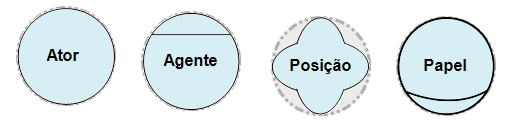
\includegraphics[keepaspectratio=true,scale=1.0]{figuras/papeisIstar.PNG}
	\caption{Símbolos que representam atores no i*.}
	\label{atoresIstar}
\end{figure}

De acordo com as definições de \cite{istarwiki20}, um  \textbf{Ator} é o termo utilizado para referir de forma genérica a qualquer unidade em que as dependências intencionais possam ser atribuídas. Os agentes, as posições e os papeis podem ser entendidos como subunidades de um ator mais complexo e sendo definidas como: 

\begin{itemize}
	\item \textbf{Agente}: Ator, normalmente quando automatizado, em algum contexto específico;
	 
	\item \textbf{Posição}: É definido como um conjunto de funções desempenhadas por um agente, também compreendido como uma abstração intermediária entre um Papel, um Agente ou Ator, sendo possível dizer que se um Agente ou Ator ocupa uma Posição, essa Posição cobre um Papel;
	
	\item \textbf{Papel}: É definido como manifestações concretas e físicas, utilizado para se referir a Atores e Agentes de \textit{Hardware}/\textit{Software}.
\end{itemize} 

No modelo Dependência Estratégica, ao existir uma cooperação entre dois atores, essa cooperação é denominada de dependência, na qual existe um ``dependente`` (\textit{depender}) e um ``de quem se depende`` (\textit{dependee}). Esses atores, \textit{depender} e \textit{dependee}, são ligados por um elo de dependência (\textit{dependum}), que pode ser uma meta a ser atingida, uma tarefa a ser realizada, um recurso a ser fornecido ou uma meta flexível a ser razoavelmente satisfeita \cite{napolitano2009estrategia}. 

\begin{figure}[h!]
	\centering
	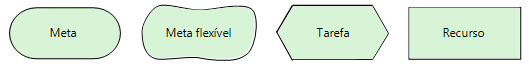
\includegraphics[keepaspectratio=true,scale=1.0]{figuras/TiposDeContribuicao.png}
	\caption{Símbolos que representam o elo de dependência.}
	\label{dependenciaIstar}
\end{figure} 

Os tipos de dependências são definidos por \cite{istarwiki20} como: 

\begin{itemize}
	
	\item \textbf{Meta}: Uma condição ou estado de desejo intencional do ator no mundo real. Os detalhes de como a meta deve ser satisfeita não são descritos, promovendo então a decomposição da mesma em uma série de alternativas.  
	 
	\item \textbf{Meta flexível}: De maneira semelhante à Meta, também representa uma condição ou estado de desejo intencional do ator no mundo real. Entretanto, os detalhes de como a meta flexível deve ser satisfeita não são definidos a princípio, sendo então sujeitos a interpretação. Para verificar se uma meta flexível foi satisfeita, utiliza-se os termos ``satisfeita a contento`` ou ``razoavelmente satisfeita``, pois metas flexíveis não possuem critérios claramente definidos. 
	
	\item \textbf{Tarefa}: Representa a realização de algo em forma particular por um ator. Uma tarefa também pode ser decomposta em subtarefas mais específicas. 
	
	\item \textbf{Recurso}: Representa uma entidade física ou informativa, pressupõe-se, então, que não existe nenhum problema ou questões abertas sobre como a recurso será alcançado.
	 
\end{itemize}

A partir das definições dos tipos de dependência e dos atores é possível modelar a relação de dependência entre dois ou mais atores. Como apresentado no exemplo da Figura \ref{exemploTipoDeDepencia}, na qual, na modelagem, existem dois atores, \textbf{Titular do cartão}, e \textbf{Banco}, sendo possível perceber a existência dos quatro tipos de dependência: dependência por recurso, dependência por tarefa, dependência por meta flexível e dependência por meta.  

\begin{figure}[h!]
	\centering
	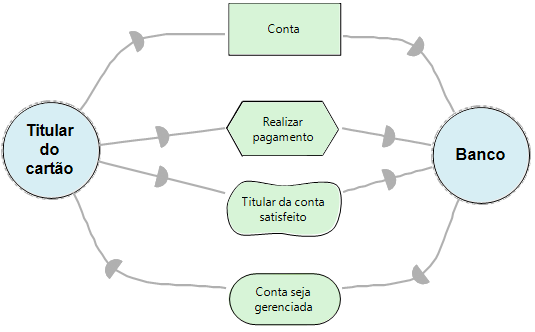
\includegraphics[keepaspectratio=true,scale=1.0]{figuras/ExemploTiposDeDependecias.PNG}
	\caption{Exemplo dos tipos de dependência entre o Títular do cartão e o Banco.}
	\label{exemploTipoDeDepencia}
\end{figure} 

\begin{itemize}
	
	\item \textbf{Dependência por recurso}: Neste tipo de dependência, o \textit{depender} depende do \textit{dependee} para que ocorra a disponibilidade do recurso. Ao determinar essa dependência, o \textit{depender} pode utilizar a entidade como um recurso \cite{istarwiki20}. No contexto da figura \ref{exemploTipoDeDepencia}, esse elo existe através do recurso \textbf{Conta}. O \textbf{Títular do cartão} é o \textit{depender}, ou seja, possui uma relação de dependência com o \textbf{Banco} (\textit{dependee}) para que o recurso, \textbf{Conta}, seja fornecido.
	
	\item \textbf{Dependência por tarefa}: Neste tipo de dependência, o \textit{depender} depende do \textit{dependee} para realização da tarefa. A tarefa pode ser entendida como uma restrição imposta pelo \textit{depender} ao \textit{dependee}, na qual o \textit{dependee} possui certa liberdade de ação dentro dessas restrições \cite{istarwiki20}. No contexto da Figura \ref{exemploTipoDeDepencia}, esse elo existe através da tarefa \textbf{Realizar pagamento}, onde o \textbf{Títular do cartão} é o \textit{depender}. Esse último depende da disponibilização do \textbf{Banco} para \textbf{Realizar pagamento} ao \textbf{Banco}. 
	
	\item \textbf{Dependência por meta flexível}: Neste tipo de dependência, o \textit{depender} depende do \textit{dependee} para que alguma tarefa seja realizada para que a meta flexível possa ser ``satisfeita a contento`` ou ``razoavelmente satisfeita`` \cite{istarwiki20}. O \textit{depender} determina se a meta flexível será alcançada ou não utilizando as habilidades e conhecimentos do \textit{dependee} \cite{napolitano2009estrategia}. No contexto da Figura \ref{exemploTipoDeDepencia}, esse elo existe através da meta flexível \textbf{Titular da conta satisfeito}. Nesse caso, o \textbf{Títular do cartão} é o \textit{depender}. Ele depende da forma como o serviço do \textbf{Banco} é prestado para que o \textit{depender} possa decidir se a meta flexível será alcançada.
	
	\item \textbf{Dependência por meta}: Neste tipo de dependência, o \textit{depender} depente do \textit{dependee} para que um estado no mundo real seja alcançado. O \textit{dependee} possui total liberdade para tomar as decisões necessárias para atingir a meta. O \textit{depender} não se preocupa com o quanto o \textit{dependee} destina-se em satisfazer a meta \cite{istarwiki20}. No contexto da Figura \ref{exemploTipoDeDepencia}, esse elo existe através da meta \textbf{Conta seja gerenciada},  \textbf{Banco} é o \textit{depender}, pois, espera-se que o \textbf{Títular do cartão} tenha capacidade de gerir sua própria conta, através dos recursos fornecidos pelo \textbf{Banco}. 
	
\end{itemize}

\subsection{Modelo de Razão Estratégica - SR}
\label{subsec:SR}

O modelo SR apresenta de forma gráfica, com vários tipos de nós (Meta, Tarefa, Recurso e Meta flexível)\footnote[1]{Os tipos de nós possuem as mesmas definições que os tipos de dependências no Modelo de Dependência Estratégica (SD) descritos na Subseção \ref{subsec:SD}} e links (links de meio-fim, links de decomposição de tarefas e links de contribuição), os quais servem como estrutura representacional que expressam as razões por trás das dependências \cite{istarwiki20}.

O modelo tem o objetivo principal de representar, de forma detalhada, as estratégias internas dos atores em função dos elementos do processo, das alternativas e das decisões por trás do processo, Essas estratégias internas dos atores representam como as metas são alcançadas, os recursos são disponibilizados, e as metas flexíveis são refinadas e operacionalizadas \cite{napolitano2009estrategia}.  

De acordo com \cite{istarwiki20}, os tipos de \textit{links} são definidos como: 

\pagebreak

\begin{itemize}
	
	\item \textbf{\textit{link} de meio-fim}: Representado graficamente por uma seta direcionada para o nó fim. O ``\textbf{meio}`` normalmente é expresso por uma tarefa, que define o ``como`` fazer algo. O " \textbf{fim}`` expressa à meta a ser alcançada.
\end{itemize}

\begin{figure}[h!]
	\centering
	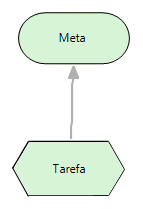
\includegraphics[keepaspectratio=true,scale=0.9]{figuras/meioFim.PNG}
	\caption{Notação gráfica para o \textit{link} de meio-fim. Adaptado de \cite{istarwiki20}.}
	\label{meiofim}
\end{figure} 

\begin{itemize}	
	\item \textbf{\textit{link} de decomposição}: Uma tarefa pode ser decomposta em submeta, subtarefa, recurso ou meta flexível. A representação gráfica para um \textit{link} de decomposição é um segmento de reta com um pequeno corte perpendicular, como apresentado na Figura \ref{decomposicaoLink}.    
\end{itemize}	

\begin{figure}[h!]
		\centering
		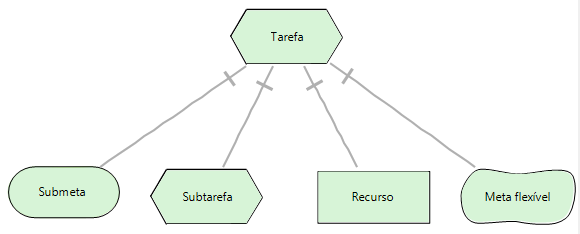
\includegraphics[keepaspectratio=true,scale=1.0]{figuras/decomposicaoLink.PNG}
		\caption{Notação gráfica para o \textit{link} de decomposição. Adaptado de \cite{istarwiki20}.}
		\label{decomposicaoLink}
\end{figure}

\begin{itemize}		
	\item \textbf{\textit{links} de contribuição}: Os tipos de contribuições\footnote[1]{A definição de cada tipo de contribuição é a mesma dada por Chung em \cite{chung2012non}, como visto na Tabela \ref{tiposDeContribuições}, que detalha os tipos de contribuições para o NFR Framework.} entre as metas flexíveis são: \textit{Make}, \textit{Some+}, \textit{Help}, \textit{Unknown}, \textit{Break}, \textit{Some-}, \textit{Hurt}, \textit{Or} e \textit{And}. 
\end{itemize}


\section{FURPS}
\label{sec:furps}

O termo FURPS é um acrônimo que define um modelo de atributo de qualidade, esse acrônimo é composto por cinco atributos de qualidade, sendo eles: (i) Funcionalidade (do inglês, \textit{Functionality}), (ii) Usabilidade (do inglês, \textit{Usability}), Confiabilidade (do inglês, \textit{Reliability}), Desempenho (do inglês, \textit{Performance}) e Suportabilidade (do inglês, \textit{Supportability}) \cite{umar2011analyzing}.

\subsection{Funcionalidade}
\label{subsec:funcionalidade}

São os requisitos funcionais de uma aplicação de software. A funcionalidade está diretamente ligada ao comportamento do software e à interação do usuário com o software \cite{cintra2006implementaccao}.

Por definição, funcionalidade é a capacidade do software de promover funções que atendam às necessidades explícitas e implícitas quando o software estiver sendo utilizado, de acordo com os cenários especificados \cite{qualidadeDeProdutoNBR}.

\subsection{Usabilidade}
\label{subsec:usabilidade}

A usabilidade faz parte do conjunto dos RNFs de uma aplicação de software. Considera-se a experiência do usuário em manipular um computador, a experiência do usuário na utilização do software, a estética da interface para o usuário e para o contexto ao qual a aplicação foi desenvolvida \cite{cintra2006implementaccao}.

Por definição, usabilidade é a capacidade do software de ser compreendido, aprendido, operado e atraente ao usuário, quando o software estiver sendo utilizado de acordo com os cenários especificados \cite{qualidadeDeProdutoNBR}.


\subsection{Confiabilidade}
\label{subsec:confiabilidade}

A confiabilidade faz parte do conjunto dos RNFs de uma aplicação de software. Considera-se a prevenção de falhas, capacidade, do software se recuperar de um erro, a precisão e o tempo entre falhas (\textit{Mean Time Between Failure} (MTBF)) \cite{cintra2006implementaccao}.

Por definição confiabilidade, é a capacidade do software em manter o nível de desempenho esperado, quando o software estiver sendo utilizado de acordo com os cenários especificados \cite{qualidadeDeProdutoNBR}.  

\subsection{Desempenho}
\label{subsec:desempenho}

O desempenho faz parte do conjunto dos RNFs de uma aplicação de software. Considera-se o tempo de recuperação e o tempo de resposta do software, a taxa de transferência de dados (do inglês, \textit{troughput}) \footnote[1]{Quantidade de dados que pode ser tranferidos de um lugar para o outro em um espaço de tempo previamente especificado.}. Capacidade do software de utilizar os recursos do sistema operacional, dentre outros \cite{cintra2006implementaccao}.

Por definição desempenho, é o nível como o software atende às necessidades, representado por um conjunto específico da valores para cada característica especificada para a execução do software. \cite{qualidadeDeProdutoNBR}.  

\subsection{Suportabilidade}
\label{subsec:suportabilidade}

Suportabilidade faz parte do conjunto dos RNFs de uma aplicação de software. Considera-se a capacidade de adaptabilidade, a possibilidade de realizar manutenções corretivas e evolutivas, a flexibilidade de configuração, de instalação e a internacionalização no sistema \cite{cintra2006implementaccao}.

\section{Arquitetura de Software}
\label{sec:arquitetura}

O conceito de \textit{design} de software surgiu da década de 1970, quando os pesquisadores da época acreditavam que o \textit{design} era uma atividade separada da implementação, exigindo notações, técnicas e ferramentas específicas. Foi somente a partir da década de 1990 que se utilizou o termo arquitetura de software em contraste com \textit{design} de software, para indicar noções de codificação, abstrações, padrões e treinamentos formais de arquitetos de software \cite{perry1992foundations}.

O termo arquitetura de software é definido por \cite{shaw1996software}, como o entendimento do sistema em termos de seus componentes computacionais e os relacionamentos entre os componentes, os padrões que guiam a composição organizacional dos componentes, bem como as decisões de restrições arquiteturais. 

As arquiteturas de software são projetadas de acordo com algum princípio de estruturação genérico, sendo esses princípios chamados de padrões arquiteturais \cite{buschmann1996system}. 

Os padrões arquiteturais são modelos para arquiteturas concretas de software, expressando a estrutura essencial para o desenvolvimento de um produto de software. O padrão fornece um conjunto de subsistemas predefinidos, incluindo regras e diretrizes para organizar as relações entre eles, além de especificar suas responsabilidades \cite{buschmann1996system}. 

A seleção de um padrão arquitetural é uma atividade fundamental ao desenvolver um sistema de software, sendo apropriado entender que cada padrão auxilia o desenvolvedor a alcançar uma propriedade de sistema específica. Dentre o conjunto dos padrões arquiteturais, existem padrões que auxiliam em propriedades similares e podem ser agrupados em categoria, sendo elas \cite{buschmann1996system}:.

\begin{itemize}
	
	\item Da lama à estrutura;
	
	\item Sistemas distribuídos;
	
	\item Sistemas interativos, e
	
	\item Sistemas adaptáveis.

\end{itemize}

A Tabela \ref{categoriasDePadroesArquiteturais} apresenta detalhadamente os quatro tipos de categorias para os padrões arquiteturais, definidos por \cite{buschmann1996system} e seus respectivos padrões.

\begin{table}[h!]
	\centering
	\caption{Descrição e padrões das quatro categorias de padrões arquiteturais.}
	\label{categoriasDePadroesArquiteturais}
	\begin{tabular}{@{}ccc@{}}
		\hline
		\textbf{Categoria} & \textbf{Descrição} & \textbf{Padrões} \\ \hline
		\begin{tabular}[c]{@{}c@{}}Da lama à \\ estrutura\end{tabular} & \begin{tabular}[c]{@{}c@{}}Confere suporte ao desenvolvedor, evitando um \\ "mar" de componentes ou objetos. Os padrões\\ dessa categoria suportam uma decomposição\\  controlada de uma tarefa geral em\\  subtarefas cooperantes.\end{tabular} & \begin{tabular}[c]{@{}c@{}}Padrão Layers\\ \\ \\ Padrão \\ Pipe-and-Filter\\ \\ \\ Padrão Blackboard\end{tabular} \\ \hline
		\begin{tabular}[c]{@{}c@{}}Sistemas \\ distribuídos\end{tabular} & \begin{tabular}[c]{@{}c@{}}O conjunto de sistemas interligados \\ que compartilham\\ processamento entre si.\end{tabular} & Broker \\ \hline
		\begin{tabular}[c]{@{}c@{}}Sistemas \\ interativos\end{tabular} & \begin{tabular}[c]{@{}c@{}}O conjunto de padrões que suportam a \\ estruturação de sistemas de software \\ os quais apresentam \\ a interação humano-computador.\end{tabular} & \begin{tabular}[c]{@{}c@{}}Model-View-\\ Controller\\ \\ \\ Presentation-\\ Abstraction-\\ Control\end{tabular} \\ \hline
		\begin{tabular}[c]{@{}c@{}}Sistemas \\ adaptáveis\end{tabular} & \begin{tabular}[c]{@{}c@{}}O conjunto de padrões que suportam, \\a adaptabilidade, a evolução tecnológica\\ e a alteração nos requisitos funcionais.\end{tabular} & \begin{tabular}[c]{@{}c@{}}Mircokernel\\ \\ \\ Reflection\end{tabular} \\ \hline
	\end{tabular}
\end{table}

\pagebreak

Devido ao foco do presente trabalho ser a construção de um catálogo de segurança para o padrão arquitetural MVC, a Subseção \ref{subsec:mvc} detalha este padrão arquitetural. 


\subsection{MVC: Model-View-Controller}
\label{subsec:mvc}

O MVC divide a aplicação em três componentes: (i) a \textit{Model}, a qual contém os dados e as funcionalidades, entendida como a camada de manipulação dos dados, (ii) a \textit{View}, componente responsável por apresentar as informações para o usuário, e (iii) a \textit{Controller}, responsável por receber e controlar as requisições de entrada do usuário, realizando o controle de qual \textit{model} usar e qual \textit{view} será mostrada ao usuário \cite{buschmann1996system}.  

\subsubsection{Model}

A \textit{Model} realiza o encapsulamento dos dados da aplicação, e detalha todo o comportamento funcional da aplicação. Este componente também realiza a exportação dos procedimentos para que a \textit{Controller} possa chamar esses procedimentos de acordo com as necessidades do usuário \cite{buschmann1996system}.

É também na \textit{Model} que ficam os registros de todos os outros componentes. Esses registros são mantidos através do mecanismo de troca de propagação \cite{buschmann1996system}. 

A Tabela \ref{responsabilidadeColaboradorModel} resume os principais aspectos da \textit{Model}, tratando de suas responsabilidades e seus colaboradores. 

\begin{table}[h!]
	\centering
	\caption{Responsabilidades e colaboradores da \textit{Model} \cite{buschmann1996system}.}
	\label{responsabilidadeColaboradorModel}
	\begin{tabular}{@{}ll@{}}
		\hline
		\textbf{Responsabilidades} &  \multicolumn{1}{c} \textbf{Colaboradores} \\ \hline
		\begin{tabular}[c]{@{}l@{}}- Fornecer o núcleo funcional da aplicação\\ - Registrar visualizações e controladores dependentes\\ - Notificar componentes dependentes sobre mudanças de dados\end{tabular} & \begin{tabular}[c]{@{}l@{}}\textit{View}\\ \textit{Controller}\end{tabular} \\ \hline
	\end{tabular}
\end{table}

\subsubsection{View}

A \textit{View} é o componente responsável por apresentar as informações ao usuário, recuperando os dados da \textit{Model} através de procedimentos de atualização que são ativados pelo mecanismo de propagação de mudanças. A \textit{View} também possui um relacionamento de 1 para 1, com a \textit{Controller}, pois fornece procedimentos para a \textit{Controller} manipular as exibições da \textit{View} \cite{buschmann1996system}.

A Tabela \ref{responsabilidadeColaboradorView} resume os principais aspectos da \textit{View}, tratando de suas responsabilidades e seus colaboradores. 

\begin{table}[h!]
	\centering
	\caption{Responsabilidades e colaboradores da \textit{View} \cite{buschmann1996system}.}
	\label{responsabilidadeColaboradorView}
	\begin{tabular}{@{}ll@{}}
		\hline
		\textbf{Responsabilidades} & \textbf{Colaboradores} \\ \hline
		\begin{tabular}[c]{@{}l@{}}- Inicializar o controlador associado\\ - Exibir informações ao usuário\\ - Implementar o procedimento de atualização\\ - Recuperar dados da \textit{Model}\end{tabular} & \begin{tabular}[c]{@{}l@{}}\textit{Model}\\ \textit{Controller}\end{tabular} \\ \hline
	\end{tabular}
\end{table}

\subsubsection{Controller}

A \textit{Controller} trata as entradas do usuário como eventos. As controladoras desses eventos recebem um pedido da \textit{View}. Nesse caso, um procedimento específico na \textit{Controller} trata esse pedido e realiza uma chamada de um procedimento na \textit{Model}. A \textit{Controller} basicamente traduz os pedidos de eventos para a \textit{Model}, sendo que, a cada pedido existe uma \textit{view} associada. 

A Tabela \ref{responsabilidadeColaboradorController} resume os principais aspectos da \textit{Controller}, tratando de suas responsabilidades e seus colaboradores. 

\begin{table}[h!]
	\centering
	\caption{Responsabilidades e colaboradores da \textit{Controller} \cite{buschmann1996system}.}
	\label{responsabilidadeColaboradorController}
	\begin{tabular}{@{}ll@{}}
		\hline
		\textbf{Responsabilidades}                    & \textbf{Colaboradores}                                                        \\ \hline
		\begin{tabular}[c]{@{}l@{}}- Aceitar entrada do usuário como eventos\\ - Traduzir os eventos para a \textit{Model} ou exibir os pedidos para a \textit{View}\\ - Se necessário, implementar prodecimentos de atualização\end{tabular} & \begin{tabular}[c]{@{}l@{}}\textit{Model}\\ \textit{View}\end{tabular} \\ \hline
	\end{tabular}
\end{table}

\subsubsection{Fluxo de interação entre os componentes}

Tão importante quanto a compreensão de cada componente é compreender o fluxo de interação entre esses componentes e suas interações diretas e indiretas. A Figura \ref{DiagramaDeClasseMVC} representa os três componentes e suas interações, através da notação da UML. Conforme representado, dentro de um pacote da \textit{Model} existe uma classe exemplo, cujo o nome é \textit{Model.Class}, possuindo relações de contribuição com o pacote \textit{Controller}, através da classe \textit{ManipuladoraDeDados.Class}. De forma semelhante, existe a relação entre a \textit{Controller} e a \textit{View} entre as classes  \textit{ManipuladoraDeDados.Class} e \textit{GUI.Class}. Os nomes atribuídos na diagramação são para auxiliar a compreensão. 

\begin{figure}[h!]
	\centering
	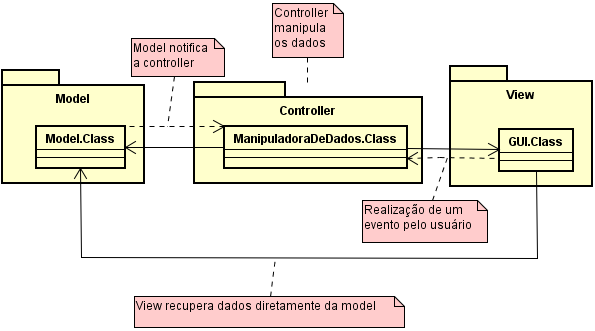
\includegraphics[keepaspectratio=true,scale=0.9]{figuras/DiagramaDeClasseMVC.PNG}
	\caption{Diagrama de classes representando a interação entre os componentes no padrão arquitetural MVC. Adaptado de \cite{durelli2008proposta}.}
	\label{DiagramaDeClasseMVC}
\end{figure}

\pagebreak

A Figura \ref{DiagramaDeSequenciaMVC} é um diagrama de sequência que representa o fluxo dos eventos em um cenário exemplo, no qual a \textit{Controller} interage diretamente com a \textit{Model} e \textit{View}, sendo que o usuário entra com alguma informação e aguarda o retorno da aplicação. 


\begin{figure}[h!]
	\centering
	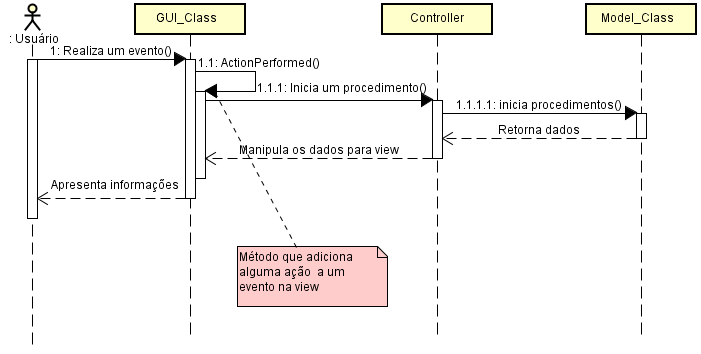
\includegraphics[keepaspectratio=true,scale=0.8]{figuras/DiagramaDeSequenciaMVC.PNG}
	\caption{Diagrama de sequência para o padrão arquitetural MVC. Adaptado de \cite{durelli2008proposta} e \cite{buschmann1996system}.}
	\label{DiagramaDeSequenciaMVC}
\end{figure}

\pagebreak

\section{Segurança vista como um RNF}
\label{sec:seguranca}

Tratando a Segurança como um RNF, pode-se entender a mesma como estando associadas a vários outros RNFs. Dessa forma, podemos entender os RNFs associados à Segurança como sendo restrições, as quais realizam operacionalizações e satisfazem as metas de segurança, estabelecidas pelos engenheiros de requisitos e/ou engenheiros de software. Esse conjunto de  RNFs devem expressar de maneira precisa e não ambígua as metas de segurança de uma aplicação, fornecendo uma especificação para alcançar a meta deseja \cite{haley2006framework}.  

Existem diversas definições de Segurança. De forma simplificada, Segurança, no contexto de Segurança da Informação, significa proteger a informação \cite{chung2012non}. O presente trabalho fundamenta-se nos conceitos de \cite{chung2012non} e \cite{sullivan2011web} como base para conceituar, Segurança, orientando-se por três conceitos conhecidos como CIA (\textit{Confidentiality}, \textit{Integrity}, \textit{Availability}) . 

Diante do exposto, para a definição seguindo os fundamentos de \cite{chung2012non}, segurança se baseia em: 

\begin{itemize}
	\item \textbf{Confidencialidade} (do inglês, \textit{Confidenciality}): Proteção da informação para evitar que as informações armazenadas ou transmitidas não sejam vistas ou interpretadas por terceiros, sendo somente o usuário principal e o destinatário. Deve-se prover essa proteção da informação através de algoritmos de criptografia \cite{chung2012non} \cite{silva2007arquitetura}. 
	
	\item \textbf{Integridade} (do inglês, \textit{Integrity}): Proteção contra qualquer tipo de atualização e/ou adulteração não autorizada. Certifica-se que essa proteção seja garantida contra todo tipo de modificação acidental ou maliciosa, garantindo que a informação percorra todo o trajeto entre o usuário principal e um destinatário \cite{chung2012non} \cite{silva2007arquitetura}. 
	
	\item \textbf{Disponibilidade} (do inglês, \textit{Availability}): Proteção contra a interrupção do serviço, no momento em que o usuário principal estiver necessitando da utilização do serviço \cite{chung2012non} \cite{silva2007arquitetura}.
	  
\end{itemize}


O CIA pode ser abstraído em metas flexíveis de Segurança. Logo após, essas metas flexíveis devem ser capturadas e organizadas em um catálogo de Segurança, promovendo um conjunto rico de alternativas e pontos de verificação para se proteger contra a negligencia de pontos relevantes, e para a segurança da informação em uma aplicação. Como apresentado na Figura \ref{catalogoSegurancaChung},  abaixo de cada conceito chave de Segurança, existem seus subtipos. 

Apresentados em  verde na Figura \ref{catalogoSegurancaChung} estão outras características dos requisitos de Segurança, sendo um dos mais relevantes o ``operacional``, que possui como subtipo ``segurança operacional`` referindo-se, diretamente, à Segurança da Informação \cite{chung2012non}.

Os subtipos das ``características dos RNF``, de acordo com \cite{chung2012non}, podem ser ``ciclo de vida``, ``operacional \footnote[1]{Operação realizada por uma aplicação de software em tempo de execução \cite{chung2012non}.}``, ``desenvolvimento \footnote[2]{Estágios de desenvolvimento \cite{chung2012non}.}``, ``interna-externa \footnote[3]{Refere-se a confidencialidade dos itens de informação do sistema \cite{chung2012non}.}``, ``interna `` e ``externa``.

\begin{figure}[h!]
	\centering
	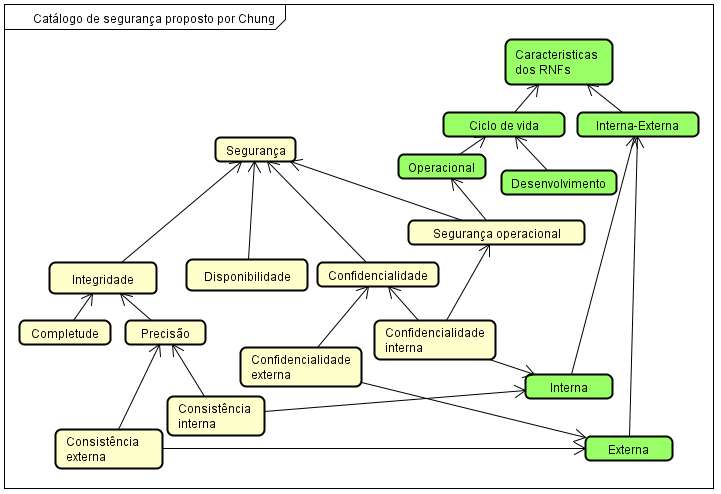
\includegraphics[keepaspectratio=true,scale=0.9]{figuras/catalogoSegurancaChung.PNG}
	\caption{Catálogo de Segurança. Fonte: \cite{chung2012non}.}
	\label{catalogoSegurancaChung}
\end{figure}

É de extrema importância entender os subtipos de cada conceito. Portanto, as subseções a seguir fazem uma breve apresentação sobre os conceitos de Confiabilidade e Integridade. 

\subsection{Confidencialidade}
\label{subsec:confidencialidade}

De acordo com \cite{reis10classificaccao}, em Confidencialidade, podem ser definidos conceitos sobre o tipo de Segurança, sendo eles:

\begin{itemize}
	\item \textbf{Irrestrito}: Tipo de informação pública. 
	
	\item \textbf{Interna}: Tipo de informação que seu acesso deve ser evitado por público externo. Caso este tipo de informação seja disponibilizado, por erro interno ou por ataque malicioso, não causa impacto algum ao mantenedor da informação.
	
	\item \textbf{Confidencial}: Tipo de informação interna, a qual, uma vez disponibilizada ao público externo, por erro interno ou ataque malicioso, pode gerar vantagens a concorrentes e, consequentemente perda de usuários/clientes. 
	
	\item \textbf{Secreta}: Tipo de informação interna, restrita a um conjunto específico de usuários, a qual, uma vez disponibilizada tanto ao público externo, quanto ao público interno não definidos, pode causar grandes danos. A integridade dessa informação deve ser mantida a qualquer custo.
\end{itemize} 

A Confidencialidade possui os subtipos ``confidencialidade interna`` e ``confidencialidade externa`` conforme ilustra a Figura \ref{catalogoSegurancaChung}.
 

\subsection{Integridade}
\label{subsec:integridade}
 
Definida através dos conceitos Precisão e Completude, por \cite{chung2012non}, onde: 

\textbf{Precisão}: Pode ser entendida como qualquer atributo semântico, que fundamenta uma informação \cite{chung2012non}, ou seja, a garantia que um requisito da informação seja descrito com precisão de acordo com, suas especificações. 

\begin{itemize}
	\item \textbf{Propriedade da precisão}: Garantir que objetos sejam instanciados da maneira correta. 
	
	\item \textbf{Valor de precisão}: Garantir que os valores retornados pelas operações possuem a precisão desejada.
	
	\item \textbf{Precisão de um para um}: Garantir que um único objeto esteja ligado a uma única entidade do domínio. 
	
	\item \textbf{Consistência interna}: Garantir que os valores do mundo real sejam correspondentes aos valores do sistema.
\end{itemize}

\textbf{Completude}: Garantir que o RNF esteja completo \cite{chung2012non}. 

\section{Resumo do capítulo}

Neste Capítulo, foi abordado os conceitos fundamentais para a construção do catálogo de segurança, foi introduzidos os conceitos chaves da Engenharia de Requisitos e aprofundando em uma de suas áreas que é a Engenharia de Requisitos Orientada à Meta, para compreendermos o conceito de meta e as suas responsabilidades, partimos então para uma visão dos requisitos, focando somente nos requisitos não-funcionais, logo em seguida foi apresentado as características e notações dos modelos intencionais NFR \textit{Framework} e o i*, bem como a apresentação do FURPS. 

Os conceitos de arquitetura de software também, foram apresentados neste Capítulo, pois são de extrema importância, para o entendimento do padrão arquitetural MVC, ao qual o catálogo de segurança é voltado, Por fim foi apresentado a visão dos requisitos de segurança como RNFs, onde foi apresentado os conceitos chave e suas definições na área de segurança, para a construção do catálogo. 



\chapter{Suporte Tecnológico}
\label{chap:suporteTecnologico}

Neste Capítulo, são apresentadas as ferramentas de software utilizadas para dar suporte ao desenvolvimento deste trabalho. A seção \ref{sec:ferramentasModelagem} apresenta uma breve descrição das ferramentas utilizadas na modelagem dos diagramas e mapas mentais. A seção \ref{sec:ferramentasDesenvolvimento} apresenta as ferramentas de suporte à escrita, e para a realização do controle de versão. A seção \ref{sec:ferramentasParaDesenvolvimentoWebApp} apresenta as ferramentas que serão utilizadas para o desenvolvimento da aplicação web durante a execução do TCC2.  

\section{Ferramentas de modelagem}
\label{sec:ferramentasModelagem}

\begin{itemize}
	\item \textbf{Astah Professional}: é uma ferramenta de modelagem de diagramas dinâmicos e estáticos, que suporta a UML 2.x, \textit{Entity Relationship Diagram} (ERD), \textit{Data Flow Diagram} (DFD), fluxogramas, mapas mentais, e a engenharia reversa para as linguagens Java, C\# e C++ \cite{astah}. A versão utilizada foi a v7.2.0 com licença de estudante, para modelagem dos diagramas da UML e mapas mentais.   
	
	\item \textbf{StarUML}: É um software \textit{open source} para modelagem de diagramas, na notação UML/\textit{Model Driven Architecture} (MDA). A proposta da ferramenta é tornar-se uma ferramenta gratuita que substitua as plataformas comerciais \cite{starUML}. A versão utilizada é a versão v1.0, pois suporta o \textit{plug-in} RE-Tools, o qual permite a modelagem do SIGs para o NFR Framework. 
	
	\item \textbf{OpenOME}: É uma ferramenta \textit{open source} de modelagem para apoiar a Engenharia Requisitos Orientada à Meta, orientada a agente e orientada a aspectos. Promove ao desenvolvedor um vínculo entre os requisitos e as especificações e as fases do \textit{design} arquitetural \cite{openOME}. A versão utilizada é a v3.4.1, para modelagem na notação do i*. 
	
	\item \textbf{Xmind}: É um software proprietário para criação de mapas mentais e suporte na criação de \textit{brainstorming} \cite{xMind}. A versão utilizada é o XMind 8 Update 2, permitindo a criação de mapas mentais. 
	
	\item \textbf{Bizagi Modeler}: É uma ferramenta gratuita utilizada para modelagem de processos de negócio, utilizando notação BPMN. É eleita pela comunidade a mais potente e fácil de utilizar do mercado. A versão utilizada é a versão 3.1, para a modelagem do fluxo de desenvolvimento da monografia \cite{bizagi}. 
	
	\item \textbf{RE-Tools}: É um conjunto de ferramentas \textit{open source} utilizado para a modelagem de diferentes aspectos das organizações e de seus sistemas, durante a realização das atividades da engenharia de requisitos, possuindo suporte para as notações do (i) NFR Framework, (ii) i*, (iii) \textit{Knowledge Acquisition in autOmated Specification} (KAOS), (iv) \textit{Problem Frames}, (v) UML e (vi) BPMN \cite{reTools} \cite{supakkul2012re}.
	
	Esse conjunto de ferramentas vem sendo utilizado para o ensino da Engenharia de Requisitos em cursos na Universidade de Trento (Itália), Universidade do Texas em Dallas (Estados Unidos) e na Universidade de Brasília (Brasil), além de estar envolvida em pesquisas no Brasil, Austrália, Canadá, China, França, Reino Unido e Estados Unidos \cite{supakkul2012re}. 
	
	No presente trabalho a versão do \textit{plug-in} utilizada foi a v3.0.2, para modelagem do gráfico de SIGs. 
\end{itemize}

\section{Ferramentas para desenvolvimento da monografia}
\label{sec:ferramentasDesenvolvimento}

\begin{itemize}
	
	\item \textbf{Git}: É um sistema \textit{open source} que suporta o controle de versão distribuído \cite{git}. A versão utilizada é a v2.13.0 para realizar o controle de versão da parte escrita da monografia. 
	
	\item \textbf{GitHub}: O GitHub é uma plataforma de hospedagem de código para controle de versão utilizando o Git, através do GitHub é possível criar uma conta para armazenar o código fonte de projetos em repositórios gratuitos e privados \cite{github}. Utilizado para hospedar o repositório público para o controle de versão da monografia, a versão utilizada é a v1.0.13.
	
	\item \LaTeX\ : É um sistema que permite a elaboração de textos em alta qualidade, através do programa de diagramação de textos TEX \cite{latex}. A versão utilizada é a v5.6.2 utilizado no desenvolvimento da parte escrita da monografia. 
	
\end{itemize}

\section{Ferramentas para o desenvolvimento da aplicação web}
\label{sec:ferramentasParaDesenvolvimentoWebApp}

O Git e o GitHub também serão utilizados para realização do controle de versão de código no desenvolvimento do software.

\begin{itemize}
	
	\item \textbf{Linux Mint 18.3 Sylvia}: É uma distribuição linux baseada no Ubuntu 16.04 LTS é a terceira e última versão do ciclo da série 18 \cite{Mint}. Essa versão será utilizada no sistema operacional para o desenvolvimento do TCC2, a versão encontra-se disponível através da URL \url{https://linuxmint.com/download.php} 
	
	\item \textbf{Sublime Text:} É um editor de textos multiplataforma. Possuindo recursos que facilitam a escrita de código, como: Minimap, edição de textos em multi-painel, salvamento automático, autocompletar, correspondência entre parenteses, dentre outros \cite{SublimeText}. A versão que será utilizada no TCC2 é a versão 3.0.
	
	\item \textbf{Ruby:} É uma linguagem de programação interpretada e multiparadigma, desenvolvida por Yukihiro “Matz” Matsumoto, unificando caraterísticas de suas linguagens favoritas (Perl, Smalltalk, Eiffel, Ada e Lisp), para formar uma linguagem que equilibra a programação funcional com a programação imperativa \cite{Ruby}. A versão da linguagem que será utilizada no TCC2 será a versão 2.5.0.
	
	\item \textbf{Ruby on Rails - (RoR):} É um  \textit{framework open source} de desenvolvimento de aplicações web, escrito em \textbf{Ruby} e baseado no padrão arquitetural MVC \cite{RoR}. A versão do \textit{framework} que será utilizada no TCC2 será a versão 5.1.5.
	
	\item \textbf{MySQL}: De acordo com a Oracle o MySQL é o Sistema de Gerenciamento de Banco de Dados (SGBD) \textit{open source} mais conhecido do mundo, além de ser uma das principais tecnologias de SGBD para desenvolvimento de aplicações web \cite{MySQL}. A versão do MySQL quer será utilizada no TCC2 será o MySQL \textit{Community Server}, sob licença GPL disponível na versão 5.7.21.
	
	\item \textbf{Bootstrap:} É um \textit{framework open source} de desenvolvimento dos componentes responsivos para interface gráfica de aplicações web, que utiliza as Linguagens HTML, CSS e JavaScript \cite{Bootstrap}. A versão que será utilizada no TCC2 será a versão 4.0.0. 
	
\end{itemize}

\section{Resumo do capítulo}

Neste capítulo, foram descritas as principais ferramentas que apoiaram o desenvolvimento do trabalho. Na seção \ref{sec:ferramentasModelagem} foi apresentada as versões e a utilização de cada ferramenta, a seção \ref{sec:ferramentasDesenvolvimento} apresenta as ferramentas utilizadas no desenvolvimento da parte escrita e o controle de versão da mesma, e a seção \ref{sec:ferramentasParaDesenvolvimentoWebApp} apresenta as ferramentas que serão utilizadas no desenvolvimento da aplicação web em tempo de execução do TCC2. 

A tabela \ref{resumo-cap-3}, resume todas as ferramentas que foram e que serão utilizadas em tempo de execução de TCC1 e TCC2. 

\begin{table}[]
	\centering
	\caption{Resumo das ferramentas de suporte.}
	\label{resumo-cap-3}
	\begin{tabular}{@{}cccc@{}}
		\toprule
		\textbf{Ferramenta} & \textbf{Versão} & \textbf{Suporte} & \textbf{Aplicabilidade} \\ \midrule
		\begin{tabular}[c]{@{}c@{}}Astah \\ Professional\end{tabular} & v7.2.0 & Modelagem & Modelagem de diagramas dinâmicos e estáticos. \\
		\rowcolor[HTML]{C0C0C0} 
		StarUML & v1.0 & Modelagem & Modelagem de diagramas na notação UML/MDA. \\
		OpenOME & v3.4.1 & Modelagem & Modelagem na notação do i*. \\
		\rowcolor[HTML]{C0C0C0} 
		Xmind & \begin{tabular}[c]{@{}c@{}}XMind 8 \\ Update 2\end{tabular} & Modelagem & Modelagem de mapas mentais. \\
		\begin{tabular}[c]{@{}c@{}}Bizagi \\ Modeler\end{tabular} & v3.1 & Modelagem & \begin{tabular}[c]{@{}c@{}}Modelagem de processos de negócio, \\ utilizando notação BPMN.\end{tabular} \\
		\rowcolor[HTML]{C0C0C0} 
		RE-Tools & v3.0.2 & Modelagem & Modelagem do gráfico de SIGs. \\
		Git & v2.13.0 & \begin{tabular}[c]{@{}c@{}}Controle de\\ versão\end{tabular} & \begin{tabular}[c]{@{}c@{}}Realização do controle de versão da escrita e \\ para o desenvolvimento da aplicação web em \\ tempo de execução do TCC2.\end{tabular} \\
		\rowcolor[HTML]{C0C0C0} 
		GitHub & v1.0.13 & \begin{tabular}[c]{@{}c@{}}Hospedagem\\ de código fonte\end{tabular} & \begin{tabular}[c]{@{}c@{}}Armazenar o código fonte da parte escrita do \\ trabalho e da aplicação web que será desenvolvida\end{tabular} \\
		LaTeX & v5.6.2 & \begin{tabular}[c]{@{}c@{}}Escrita/\\ formatação\end{tabular} & Utilizado para a escrita e formatação do texto. \\
		\rowcolor[HTML]{C0C0C0} 
		Linux Mint & \begin{tabular}[c]{@{}c@{}}v18.3 \\ Sylvia\end{tabular} & \begin{tabular}[c]{@{}c@{}}Sistema \\ Operacional\end{tabular} & \begin{tabular}[c]{@{}c@{}}Será o sistema operacional para o desenvolvimento\\ da aplicação web.\end{tabular} \\
		Sublime Text & v3.0 & \begin{tabular}[c]{@{}c@{}}Escrita de \\ código\end{tabular} & \begin{tabular}[c]{@{}c@{}}Editor de textos para escrita do código fonte \\ da aplicação web.\end{tabular} \\
		\rowcolor[HTML]{C0C0C0} 
		Ruby & v2.5.0 & \begin{tabular}[c]{@{}c@{}}Linguagem \\ de programação\end{tabular} & \begin{tabular}[c]{@{}c@{}}Linguagem de programação para desenvolvimento\\ da aplicação web.\end{tabular} \\
		RoR & v5.1.5 & Desenvolvimento & \begin{tabular}[c]{@{}c@{}}Framework de desenvolvimento web de acordo\\ com o padrão arquitetural MVC.\end{tabular} \\
		\rowcolor[HTML]{C0C0C0} 
		MySQL & v5.7.21 & Desenvolvimento & \begin{tabular}[c]{@{}c@{}}SGBD que será utilizado no desenvolvimento da \\ aplicação web.\end{tabular} \\
		Bootstrap & v4.0.0 & Desenvolvimento & \begin{tabular}[c]{@{}c@{}}Framework quer será utilizado para desenvolver\\ o front-end da aplicação web.\end{tabular} \\ \bottomrule
	\end{tabular}
\end{table}


\chapter{Metodologia}
\label{chap:metodologia}

Neste Capítulo, é apresentada a classificação de pesquisa na secção \ref{sec:classificacaoDaPesquisa}, classificando-a de acordo com a sua abordagem, sua natureza, seus objetivos e procedimentos. A seção \ref{sec:metodologiaDeDesenvolvimentoDeSoftware} apresenta a metodologia de desenvolvimento de software que será utilizada para o TCC2. A seção \ref{sec:procedimentosMetodológicos} apresenta os procedimentos metodológicos para o desenvolvimento desse trabalho, procurando detalhar o fluxo de atividades bem como o cronograma de ambos, TCC1 e TCC2.  

\section{Classificação da pesquisa}
\label{sec:classificacaoDaPesquisa}

A pesquisa científica pode ser classificada de acordo com sua abordagem, sua natureza, seus objetivos e seus procedimentos técnicos \cite{gerhardt2009metodos}. Portanto, nessa seção, procura-se enquadrar a pesquisa do presente trabalho, classificando-a quanto à Abordagem de pesquisa (seção \ref{sub:abordagemDePesquisa}); à Natureza de pesquisa (seção \ref{sub:naturezaDePesquisa}), aos Objetivos de pesquisa (seção \ref{sub:objetivosDePesquisa}) e aos Procedimentos técnicos de pesquisa (seção \ref{sub:procedimentosDePesquisa}).

\subsection{Abordagem de pesquisa}
\label{sub:abordagemDePesquisa}

Segundo \cite{gerhardt2009metodos}, a pesquisa qualitativa preocupa-se com os aspectos da realidade e que não podem ser quantificados, centrando-se na compreensão e explicação da dinâmica das relações sociais. Também possui três características fundamentais para prosseguir com os estudos \cite{mazzotti1991planejamento}, são elas:

\begin{itemize}
	\item \textit{Visão holística:} A compreensão de um comportamento ou evento só é possível com o entendimento das inter-relações que surgem dentro do contexto da pesquisa;
	\item \textit{Abordagem indutiva:} O pesquisador parte de observações mais livres, deixando que as dimensões e categorias de interesse surjam progressivamente durante todo o processo de coleta e análise dos dados;
	\item \textit{Investigação naturalística:} A intervenção do pesquisador no contexto observado é reduzida ao mínimo.
\end{itemize}

A abordagem de \textbf{pesquisa qualitativa} é utilizada na execução desta pesquisa, pois para execução da pesquisa, o autor tem a necessidade de realizar as ações de descrever os principais subtipos de RNFs de Segurança, visando a estruturação de um catálogo de Segurança utilizando o NFR \textit{Framework}, bem como compreender e explicar os impactos entre os RNFs no padrão arquitetural MVC. 

\subsection{Natureza de pesquisa}
\label{sub:naturezaDePesquisa}

Essa pesquisa é caracterizada como uma \textbf{pesquisa aplicada}, pois os conhecimentos gerados são voltados para a aplicação prática \cite{gerhardt2009metodos}, visando auxiliar os engenheiros de requisitos e engenheiros de software na especificação dos RNFs de segurança, quando uma arquitetura é imposta. 

\subsection{Objetivos de pesquisa}
\label{sub:objetivosDePesquisa}

Quanto aos objetivos, essa pesquisa pode ser classificada como \textbf{pesquisa explicativa}, pois, segundo \cite{gil2002elaborar}, “...este tipo de pesquisa preocupa-se em identificar os fatores que determinam ou que contribuem para a ocorrência dos fenômenos...”, ou seja, pretende-se explicar como o padrão arquitetural MVC pode ser impactado pelos RNFs, de acordo com o catálogo de Segurança.

\subsection{Procedimentos técnicos de pesquisa}
\label{sub:procedimentosDePesquisa}

A \textbf{pesquisa bibliográfica} é um dos procedimentos técnicos de pesquisa utilizados, como é evidente no Capítulo \ref{chap:referencialTeorico}, onde é apresentado todo o levantamento teórico que serve de insumo para a execução dessa monografia. De acordo com \cite[p.35]{fonseca2002metodologia}, “\textit{esse tipo de procedimento trata-se do levantamento de referências teóricas já analisadas, e publicadas por meio de escritos e eletrônicos, como livros, artigos científicos, páginas de web sites. Qualquer trabalho científico inicia-se com uma pesquisa bibliográfica, que permite ao pesquisador conhecer o que já estudou sobre o assunto}“.
 
Outro procedimento técnico de pesquisa adotado é a \textbf{pesquisa ação}, pois se trata de uma participação planejada do ator em uma situação problemática a ser investigada \cite{fonseca2002metodologia}. O ator participa ativamente do levantamento, adquirindo consigo uma série de conhecimentos que servirão como base para construção do catálogo de Segurança e que, em tempo de execução do TCC2, será validado, através do desenvolvimento de uma solução de software utilizando o padrão arquitetural MVC. 

\section{Metodologia de desenvolvimento de software}
\label{sec:metodologiaDeDesenvolvimentoDeSoftware}

A metodologia de desenvolvimento de software utilizada para o TCC2 será o \textbf{scrum com adaptações}, que trata-se de uma metodologia de desenvolvimento ágil utilizada para a gestão e planejamento de projetos de software \cite{schwaber2002agile}. 

\pagebreak

O scrum trata os projetos de forma iterativa e incremental, entregando ao final de cada \textit{sprint}\footnote[1]{Curto período de tempo em que são realizadas as atividades de desenvolvimento de software, é indicado que seja de 2 a 4 semanas \cite{schwaber2002agile}.} uma versão funcional do software com o incremento de uma nova funcionalidade \cite{schwaber2002agile}. Para a execução do TCC2 a \textit{sprint} terá duração de 2 semanas com inicio do desenvolvimento em Marco e finalizando no início de Junho. 

Outro conceito do scrum que será utilizado é o \textit{product backlog}\footnote[2]{Lista de funcionalidades a serem implementadas no projeto de software, não necessita estar preenchida por completo no inicio do projeto, pois essa lista cresce a medida que se aprende mais sobre o produto de software \cite{schwaber2002agile}.} Para execução do TCC2 será aplicado o conceito de \textit{product backlog}.

Com base no \textit{product backlog} o \textit{scrum team}\footnote[3]{Um time scrum é definido por uma equipe de pessoas variando de 6 a 10 pessoas \cite{schwaber2002agile}. No presente trabalho o \textit{scrum team} sofre uma adaptação para somente uma única pessoa ``o autor``, mas o termo será utilizado para referir-se diretamente ao autor.} realizará o planejamento da \textit{sprint}, de acordo com as funcionalidades mais relevantes. 

As reuniões de retrospectiva e revisão de \textit{sprint} ocorrerão duas vezes dentro da \textit{sprint}, será as reuniões semanais   de ponto de controle com os orientadores ao qual apresentará o que foi feito, o que não foi feito, e o por que não foi feito, no decorrer da \textit{sprint}. 

O Kanban um método ágil que promove ao \textit{scrum team} e aos \textit{stakeholders} do trabalho uma visão geral de gestão do estado de implementação de uma funcionalidade \cite{prikladnicki2014metodos}. Será utilizado para controle visual do fluxo das atividades, dividindo suas colunas da seguinte maneira ``fazer``, ``Fazendo`` e ``Feito``.

\section{Procedimentos Metodológicos}
\label{sec:procedimentosMetodológicos}

Para o desenvolvimento do trabalho, foram realizadas várias atividades. Essas atividades foram então organizadas como um processo de desenvolvimento, conforme ilustrado nas Figura \ref{PDM-TCC1} e \ref{PDM-TCC2}. 

Pelas diretrizes do curso de graduação em Engenharia de Software, é necessária à aprovação nas disciplinas de TCC1 e TCC2. Assim, nas próximas seções, procurou-se detalhar o fluxo de atividades que conduzirá a execução do trabalho como um todo. 

\subsection{Fluxo de atividades do o TCC1}

Este processo tem como principal objetivo a fundamentação, a elaboração e a estruturação do catálogo de Segurança para o padrão arquitetural MVC. 

\begin{figure}[h!]
	\centering
	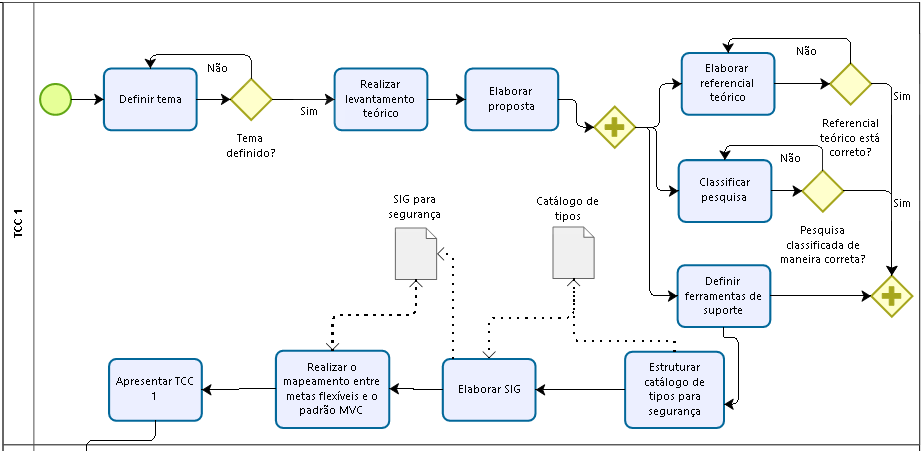
\includegraphics[keepaspectratio=true,scale=0.6]{figuras/PDM-TCC1.PNG}
	\caption{Atividades realizadas no TCC1.}
	\label{PDM-TCC1}
\end{figure}

As atividades são:

\begin{itemize}
	\item \textbf{Definir tema}: Junto com os professores orientadores desse trabalho, essa atividade teve como principal objetivo o refinamento sobre os conceitos teóricos referentes à área de interesse do autor.   
	
	\item \textbf{Realizar levantamento teórico}: Com base nos resultados obtidos da execução da atividade anterior, iniciou-se o levantamento teórico, seguindo as orientações dos orientadores. Discutiu-se sobre os aspectos fundamentais do GORE, os \textit{frameworks} que se apoiam nos conceitos do GORE, os conceitos de Arquitetura de Software e os atributos de qualidade mais relevantes para o mercado e para a academia. 
	
	\item \textbf{Elaborar proposta}: Com o conhecimento das necessidades da área de atuação desse trabalho, iniciou a elaboração da proposta de pequisa. Ficou acordado que seria utilizado o NFR Framework bem como que seria aplicado o trabalho ao mercado, tomando Segurança como o principal atributo de qualidade.  
	
	\item \textbf{Elaborar referencial teórico}: Redação dos conceitos teóricos a serem aplicados no desenvolvimento desse trabalho. 
	
	\item \textbf{Classificar pesquisa}: Redação  da classificação da pesquisa em suas dimensões. Sendo especificada quanto (i) à abordagem de pesquisa, (ii) à natureza de pesquisa, (iii) aos objetivos de pesquisa, e (iv) aos procedimentos técnicos de pesquisa.
	
	\item \textbf{Definir ferramentas de suporte}: Definição e descrição das ferramentas utilizadas no desenvolvimento desse trabalho.  
	
	\item \textbf{Estruturar catálogo de tipos de segurança}: Com base nos conceitos de Segurança apresentados por Lawrence Chung, Brian A. Nixon, Eric Yu e John Mylopoulos, no  livro: \textit{NON-FUNCTIONAL REQUIREMENTS
	IN SOFTWARE ENGINEERING}, iniciou-se a elaboraçao  do catálogo de tipos de RNFs para Segurança, e expandindo o catálogo com base em definições de subtipos de RNFs.
	
	\item \textbf{Elaborar SIG}: A partir do catálogo de Segurança, iniciou-se o processo de identificação das metas flexíveis que podem ser satisfeitas, orientando-se também pelo livro supracitado.
	
	\item \textbf{Realizar o mapeamento entre metas flexíveis e o padrão MVC}: Iniciou-se a comparação das metas flexíveis que possuiam tipo arquitetural e gerariam impactos positivos ou negativos na Segurança dos dados e da arquitetura. Caso ocorresse a identificação de outro subtipo para Segurança à atividade, ``Estruturar catálogo de tipos para Segurança`` era realizada novamente e consequentemente as atividades seguintes de acordo com a Figura \ref{PDM-TCC1}. 
	
	\item \textbf{Definir tecnologia de desenvolvimento de software}: Definir ferramentas para o desenvolvimento do software de exemplo, desenvolvido utilizando o padrão arquitetural MVC.
	
	\item \textbf{Definir metodologia de desenvolvimento de software}: Definir metodologia de desenvolvimento de software a ser utilizada.
	
	\item \textbf{Apresentar TCC 1}: Defesa do TCC1 para a banca. 
\end{itemize}

\subsection{Fluxo de Atividades do TCC2}

Este processo tem como principal objetivo a validação do catálogo proposto, através do desenvolvimento de uma aplicação de software. 

\begin{figure}[h!]
	\centering
	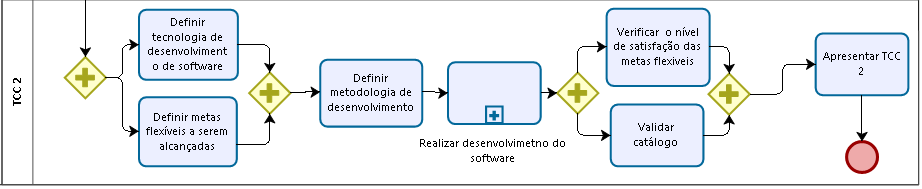
\includegraphics[keepaspectratio=true,scale=0.7]{figuras/PDM-TCC2.PNG}
	\caption{Atividades a serem realizadas no TCC2.}
	\label{PDM-TCC2}
\end{figure}

As atividades são:

\begin{itemize}
		
	\item \textbf{Definir metas flexíveis a serem alcançadas}: Definir as metas flexíveis a serem alcançadas de acordo com o cenário exemplo do software a ser desenvolvido.  
	
	\item \textbf{Macro atividade: Realizar desenvolvimento do software}: Realizar as etapas de desenvolvimento de acordo com a metodologia selecionada.
	
	\item \textbf{Verificar o nível de satisfação das metas flexíveis}: Verificar se as metas flexíveis foram alcançadas após o desenvolvimento do software.
	
	\item \textbf{Coletar as primeiras impressões da aplicação do catálogo}: Validar o catálogo de segurança porposto no TCC1 de acordo com o cenário especificado. 
	
	\item \textbf{Apresentar TCC 2}: Apresentar TCC 2 para a banca.
\end{itemize}

\subsection{Cronograma das atividades}

O cronograma apresentado no Tabela \ref{cronograma-tcc1}, organizado em meses,  procura expor como se deu a execução das atividades do TCC1. 

Observa-se que foram utilizados, além do prazo base, os meses de Janeiro e Fevereiro. Isso ocorreu para um melhor aprofundamento do tema, o qual demandou a leitura de vários materiais bibliográficos. Adicionalmente, as notações envolvidas nessa pesquisa são complexas, necessitando de um cuidado maior na escrita, facilitando o entendimento por parte dos interessados.

\begin{table}[h!]
	\centering
	\caption{Cronograma das atividades para desenvolvimento do TCC1.}
	\label{cronograma-tcc1}
	\begin{tabular}{@{}lccccccc@{}}
		\hline
		\textbf{Atividade} & \multicolumn{1}{l}{\textbf{Ago}} & \multicolumn{1}{l}{\textbf{Set}} & \multicolumn{1}{l}{\textbf{Out}} & \multicolumn{1}{l}{\textbf{Nov}} & \multicolumn{1}{l}{\textbf{Dez}} & \multicolumn{1}{l}{\textbf{Jan}} & \multicolumn{1}{l}{\textbf{Fev}} \\ \hline
		Definir tema & \textbf{x} & \textbf{} & \textbf{} & \textbf{} & \textbf{} & \textbf{} & \textbf{} \\ \hline
		Realizar levantamento teórico & \textbf{x} & \textbf{x} & \textbf{} & \textbf{} & \textbf{} & \textbf{} & \textbf{} \\ \hline
		Elaborar proposta & \textbf{x} & \textbf{x} & \textbf{x} & \textbf{} & \textbf{} & \textbf{} & \textbf{} \\ \hline
		Elaborar referencial teórico & \textbf{} & \textbf{} & \textbf{x} & \textbf{x} & \textbf{x} & \textbf{} & \textbf{} \\ \hline
		Classificar pesquisa & \textbf{} & \textbf{} & \textbf{x} & \textbf{x} & \textbf{x} & \textbf{} & \textbf{} \\ \hline
		Definir ferramentas de suporte & \textbf{} & \textbf{} & \textbf{x} & \textbf{x} & \textbf{x} & \textbf{} & \textbf{} \\ \hline
		\begin{tabular}[c]{@{}l@{}}Estruturar catálogo de tipos \\ para segurança\end{tabular} & \textbf{} & \textbf{} & \textbf{} & \textbf{} & \textbf{x} & \textbf{x} & \textbf{} \\ \hline
		Elaborar SIG & \textbf{} & \textbf{} & \textbf{} & \textbf{} & \textbf{x} & \textbf{x} & \textbf{} \\ \hline
		\begin{tabular}[c]{@{}l@{}}Realizar mapeamento entre metas\\ flexíveis e o padrão MVC\end{tabular} & \textbf{} & \textbf{} & \textbf{} & \textbf{} & \textbf{} & \textbf{x} & \textbf{x} \\ \hline
		\begin{tabular}[c]{@{}l@{}}Definir metodologia de\\ desenvolvimento de software MVC\end{tabular} & \textbf{} & \textbf{} & \textbf{} & \textbf{} & \textbf{} & \textbf{x} & \textbf{x} \\ \hline
		\begin{tabular}[c]{@{}l@{}}Definir tecnologia de desenvolvimento\\ de software\end{tabular} & \textbf{} & \textbf{} & \textbf{} & \textbf{} & \textbf{} & \textbf{x} & \textbf{x} \\ \hline
		Apresentar TCC1 & \textbf{} & \textbf{} & \textbf{} & \textbf{} & \textbf{} & \textbf{} & \textbf{x} \\ \hline
	\end{tabular}
\end{table}

Na Tabela, é apresentado um planejamento para execução das atividades referentes ao TCC2. trata-se de uma previsão, podendo ocorrer pequenos ajustes ao longo da realização do trabalho.

\begin{table}[h!]
	\centering
	\caption{Cronograma das atividades para desenvolvimento do TCC2.}
	\label{cronograma-tcc2}
	\begin{tabular}{@{}lccccc@{}}
		\hline
		\textbf{Atividade} & \multicolumn{1}{l}{\textbf{Mar}} & \multicolumn{1}{l}{\textbf{Abr}} & \multicolumn{1}{l}{\textbf{Mai}} & \multicolumn{1}{l}{\textbf{Jun}} & \multicolumn{1}{l}{\textbf{Jul}} \\ \hline
		Definir metas flexíveis a serem alcançadas & \textbf{x} & \textbf{} & \textbf{} & \textbf{} & \textbf{} \\ \hline
		Realizar desenvolvimento do software & \textbf{x} & \textbf{x} & \textbf{x} & \textbf{x} & \textbf{} \\ \hline
		\begin{tabular}[c]{@{}l@{}}Verificar o nível de satisfação das metas\\ flexíveis\end{tabular} & \textbf{} & \textbf{} & \textbf{x} & \textbf{x} & \textbf{} \\ \hline
		Coletar as primeiras impressões da \\ aplicação do catálogo & \textbf{} & \textbf{} & \textbf{} & \textbf{x} & \textbf{} \\ \hline
		Apresentar TCC 2 & \textbf{} & \textbf{} & \textbf{} & \textbf{x} & \textbf{} \\ \hline
	\end{tabular}
\end{table} 

\section{Resumo do capítulo}

Neste capitulo foi detalhada a classificação da pesquisa de acordo com seus tipos, como sendo a (i) abordagem de pesquisa, se tratando de uma pesquisa qualitativa, a (ii) Natureza de pesquisa, caraterizada como uma pesquisa aplicada, o (ii) objetivo de pesquisa, caracterizado como uma pesquisa explicativa e os (iv) procedimentos técnicos de pesquisa, caracterizados como uma pesquisa bibliográfica e a pesquisa ação. E a adaptação do Scrum como método de desenvolvimento de software e o Kanban para acompanhamento visual do andamento da implementação das funcionalidades da aplicação web.

Adicionalmente, procurou-se detalhar ambos os fluxos de atividades e cronogramas para o pleno desenvolvimento do TCC1 e TCC2, respectivamente.

\chapter{Proposta}
\label{chap:proposta}

\section{Catálogo de Segurança}

Esse catálogo de Segurança procura promover aos engenheiros de requisitos e engenheiros de software uma maior compreensão quanto às diferentes necessidades em se tratando de Segurança de Dados e Segurança em termos arquiteturais. Isso é obtido, pois o catálogo acorda os principais conceitos associados à Segurança, com base em levantamento bibliográfico, e que por isso mostram-se relevantes para o desenvolvimento de aplicações, cujo gargalo é Segurança.

Para melhor organização, o catálogo está estruturado em três níveis de detalhamento, o primeiro nível define as metas flexíveis de Segurança sem o foco em Segurança de Dados e os aspectos arquiteturais, o segundo nível realiza o mapeamento entre as metas flexíveis do primeiro nível com os aspectos arquiteturais do MVC e o terceiro nível realiza o mapeamento dos aspectos arquiteturais do MVC com as operacionalizações, de acordo com a meta flexível mapeada.

Os três níveis de detalhamento são descritos nas subseções abaixo. 

\subsection{Primeiro nível de detalhamento}
\label{sub:primeiroNivel}

O primeiro nível de detalhamento apresenta as metas flexíveis mais genéricas de Segurança de software, apoiando-se principalmente na definição na definição de Chung que se baseia em Confidencialidade, Integridade e Disponibilidade e na definição de Segurança da Informação apresentada na ISO 27001.

\begin{citacao}
	"Segurança da informação: preservação da \textbf{confidencialidade}, \textbf{integridade} e \textbf{disponibilidade} da informação; adicionalmente, outras propriedades, tais como \textbf{autenticidade}, \textbf{responsabilidade}, não repúdio e \textbf{confiabilidade}, podem também estar envolvidas." \cite[p. 2]{documentation2005information}
\end{citacao}


As metas flexíveis foram definidas de acordo com sua relação com Segurança. A meta flexível no SIG apresenta um valor número, esse valor representa a rastreabilidade do conceito da meta com sua devida referência teórica, comprovando a relação direta da meta com Segurança. a Tabela \ref{indicesDeReferencia} apresenta os identificadores para a rastreabilidade da referência teórica de uma meta flexível no SIG da Figura \ref{DetalhamentoPrimeiroNivel}. 

\begin{table}[h!]
	\centering
	\caption{Índices de rastreabilidade.}
	\label{indicesDeReferencia}
	\begin{tabular}{@{}cc@{}}
		\toprule
		\textbf{Identificador} & \textbf{Referência} \\ \midrule
		{[}1{]} & \cite{chung2012non} \\ 
		{[}2{]} & \cite{benitti2015taxonomia} \\
		{[}3{]} & \cite{documentation2005information} \\ \bottomrule
	\end{tabular}
\end{table} 

\begin{figure}[h!]
	\centering
	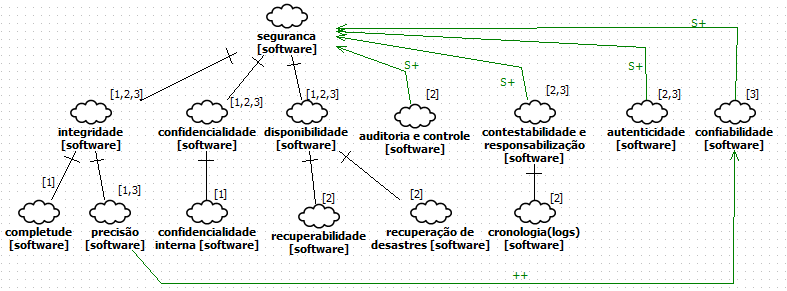
\includegraphics[keepaspectratio=true,scale=0.8]{figuras/primeiroNivel.PNG}
	\caption{Catálogo de Segurança.}
	\label{DetalhamentoPrimeiroNivel}
\end{figure}

As definições das metas flexíveis são: 

\begin{itemize}
	
	\item \textbf{integridade:} Proteção contra qualquer tipo de atualização e/ou adulteração não autorizada. Definida na seção \ref{sec:seguranca}.
	
	\begin{itemize}
		
		\item \textbf{precisão:} Pode ser entendida como qualquer atributo semântico que fundamenta uma informação. Definida na seção \ref{sec:seguranca}.
		
		\item \textbf{completude:} Garantia que o RNF esteja completo. Definida na seção \ref{sec:seguranca}.
	\end{itemize}
	
	\item \textbf{confidencialidade:} Proteção da informação para evitar que as informações armazenadas ou transmitidas não sejam vistas ou interpretadas por terceiros, sendo somente o usuário principal e o destinatário. Definida na seção \ref{sec:seguranca}.
	
	\begin{itemize}
		
		\item \textbf{confidencialidade interna:} Proteção da informação que o acesso deve ser evitado por um público externo. Definida na seção \ref{sec:seguranca}.
		
	\end{itemize}
	 
	 \item \textbf{disponibilidade:} Proteção contra a interrupção do serviço, no momento em que o usuário estiver utilizando a aplicação. Definida na seção \ref{sec:seguranca}.
	 
	 \begin{itemize}
	 		
	 		\item \textbf{recuperabilidade:} Intervalo de tempo que o software deverá estar disponível após uma falha \cite{benitti2015taxonomia}.
	 	
	 		\item \textbf{recuperação de desastres:} Políticas e procedimentos aplicados na recuperação de ``desastres`` induzidos no software por usuário ou softwares de terceiros \cite{benitti2015taxonomia}.
	 		
	 \end{itemize}
 
 	\item \textbf{auditoria e controle:} Especificação dos aspectos que devem ser contemplados para proporcionar a auditoria e o controle \cite{benitti2015taxonomia}. 
 	
 	\item  \textbf{contestabilidade e responsabilização:} Capacidade do software em quantificar as ações e eventos, com intuito de comprovar sua ocorrência \cite{benitti2015taxonomia}. 
 	
 	\begin{itemize}
 		
 		\item \textbf{cronologia(logs):} Registro de alterações no software \cite{benitti2015taxonomia}.
 		
 	\end{itemize}
 	
 	\item \textbf{autenticidade:} Pode ser entendida como a capacidade do software em identificar que um objeto ou recurso é o que ele realmente declara ser \cite{benitti2015taxonomia}. 
 	
 	\item \textbf{confiabilidade:} Pode ser entendida como a capacidade do software em realizar e manter seu funcionamento quando submetido em circunstâncias de rotina \cite{benitti2015taxonomia}. 
 	
\end{itemize}

\subsection{Segundo nível de detalhamento}
\label{sub:segundoNivel}

O segundo nível de detalhamento apresenta as metas flexíveis mais genéricas com foco na relação com Segurança de Dados e os aspectos arquiteturais do padrão MVC.  


\subsection{Terceiro nível de detalhamento}
\label{sub:terceiroNivel}

\chapter{Considerações finais}
\label{chap:consideracoesFinais}
\chapter{Suporte Tecnológico}
\label{chap:suporteTecnologico}

Neste Capítulo, são apresentadas as ferramentas de software utilizadas para dar suporte ao desenvolvimento deste trabalho. A seção \ref{sec:ferramentasModelagem} apresenta uma breve descrição das ferramentas utilizadas na modelagem dos diagramas e mapas mentais. A seção \ref{sec:ferramentasDesenvolvimento} apresenta as ferramentas de suporte à escrita, e para a realização do controle de versão. A seção \ref{sec:ferramentasParaDesenvolvimentoWebApp} apresenta as ferramentas que serão utilizadas para o desenvolvimento da aplicação web durante a execução do TCC2.  

\section{Ferramentas de Modelagem}
\label{sec:ferramentasModelagem}

\begin{itemize}
	\item \textbf{Astah Professional}: é uma ferramenta de modelagem de diagramas dinâmicos e estáticos, que suporta a UML 2.x, \textit{Entity Relationship Diagram} (ERD), \textit{Data Flow Diagram} (DFD), fluxogramas, mapas mentais, e a engenharia reversa para as linguagens Java, C\# e C++ \cite{astah}. A versão utilizada foi a v7.2.0 com licença de estudante, para modelagem dos diagramas da UML e mapas mentais.   
	
	\item \textbf{StarUML}: É um software \textit{open source} para modelagem de diagramas, na notação UML/\textit{Model Driven Architecture} (MDA). A proposta da ferramenta é tornar-se uma ferramenta gratuita que substitua as plataformas comerciais \cite{starUML}. A versão utilizada é a versão v1.0, pois suporta o \textit{plug-in} RE-Tools, o qual permite a modelagem do SIGs para o NFR Framework. 
	
	\item \textbf{OpenOME}: É uma ferramenta \textit{open source} de modelagem para apoiar a Engenharia Requisitos Orientada à Meta, orientada a agente e orientada a aspectos. Promove ao desenvolvedor um vínculo entre os requisitos e as especificações e as fases do \textit{design} arquitetural \cite{openOME}. A versão utilizada é a v3.4.1, para modelagem na notação do i*. 
	
	\item \textbf{Xmind}: É um software proprietário para criação de mapas mentais e suporte na criação de \textit{brainstorming} \cite{xMind}. A versão utilizada é o XMind 8 Update 2, permitindo a criação de mapas mentais. 
	
	\item \textbf{Bizagi Modeler}: É uma ferramenta gratuita utilizada para modelagem de processos de negócio, utilizando notação BPMN. É eleita pela comunidade a mais potente e fácil de utilizar do mercado. A versão utilizada é a versão 3.1, para a modelagem do fluxo de desenvolvimento da monografia \cite{bizagi}. 
	
	\item \textbf{RE-Tools}: É um conjunto de ferramentas \textit{open source} utilizado para a modelagem de diferentes aspectos das organizações e de seus sistemas, durante a realização das atividades da engenharia de requisitos, possuindo suporte para as notações do (i) NFR Framework, (ii) i*, (iii) \textit{Knowledge Acquisition in autOmated Specification} (KAOS), (iv) \textit{Problem Frames}, (v) UML e (vi) BPMN \cite{reTools} \cite{supakkul2012re}.
	
	Esse conjunto de ferramentas vem sendo utilizado para o ensino da Engenharia de Requisitos em cursos na Universidade de Trento (Itália), Universidade do Texas em Dallas (Estados Unidos) e na Universidade de Brasília (Brasil), além de estar envolvida em pesquisas no Brasil, Austrália, Canadá, China, França, Reino Unido e Estados Unidos \cite{supakkul2012re}. 
	
	No presente trabalho a versão do \textit{plug-in} utilizada foi a v3.0.2, para modelagem do gráfico de SIGs. 
\end{itemize}

\section{Ferramentas para Desenvolvimento da Monografia}
\label{sec:ferramentasDesenvolvimento}

\begin{itemize}
	
	\item \textbf{Git}: É um sistema \textit{open source} que suporta o controle de versão distribuído \cite{git}. A versão utilizada é a v2.13.0 para realizar o controle de versão da parte escrita da monografia. 
	
	\item \textbf{GitHub}: O GitHub é uma plataforma de hospedagem de código para controle de versão utilizando o Git, através do GitHub é possível criar uma conta para armazenar o código fonte de projetos em repositórios gratuitos e privados \cite{github}. Utilizado para hospedar o repositório público para o controle de versão da monografia, a versão utilizada é a v1.0.13.
	
	\item \LaTeX\ : É um sistema que permite a elaboração de textos em alta qualidade, através do programa de diagramação de textos TEX \cite{latex}. A versão utilizada é a v5.6.2 utilizado no desenvolvimento da parte escrita da monografia. 
	
\end{itemize}

\section{Ferramentas para o Desenvolvimento da Aplicação Web}
\label{sec:ferramentasParaDesenvolvimentoWebApp}

O Git e o GitHub também serão utilizados para realização do controle de versão de código no desenvolvimento do software.

\begin{itemize}
	
	\item \textbf{Linux Mint 18.3 Sylvia}: É uma distribuição linux baseada no Ubuntu 16.04 LTS é a terceira e última versão do ciclo da série 18 \cite{Mint}. Essa versão será utilizada no sistema operacional para o desenvolvimento do TCC2, a versão encontra-se disponível através da URL \url{https://linuxmint.com/download.php} 
	
	\item \textbf{Sublime Text:} É um editor de textos multiplataforma. Possuindo recursos que facilitam a escrita de código, como: Minimap, edição de textos em multi-painel, salvamento automático, autocompletar, correspondência entre parenteses, dentre outros \cite{SublimeText}. A versão que será utilizada no TCC2 é a versão 3.0.
	
	\item \textbf{Ruby:} É uma linguagem de programação interpretada e multiparadigma, desenvolvida por Yukihiro “Matz” Matsumoto, unificando caraterísticas de suas linguagens favoritas (Perl, Smalltalk, Eiffel, Ada e Lisp), para formar uma linguagem que equilibra a programação funcional com a programação imperativa \cite{Ruby}. A versão da linguagem que será utilizada no TCC2 será a versão 2.5.0.
	
	\item \textbf{Ruby on Rails - (RoR):} É um  \textit{framework open source} de desenvolvimento de aplicações web, escrito em \textbf{Ruby} e baseado no padrão arquitetural MVC \cite{RoR}. A versão do \textit{framework} que será utilizada no TCC2 será a versão 5.1.5.
	
	\item \textbf{MySQL}: De acordo com a Oracle o MySQL é o Sistema de Gerenciamento de Banco de Dados (SGBD) \textit{open source} mais conhecido do mundo, além de ser uma das principais tecnologias de SGBD para desenvolvimento de aplicações web \cite{MySQL}. A versão do MySQL quer será utilizada no TCC2 será o MySQL \textit{Community Server}, sob licença GPL disponível na versão 5.7.21.
	
	\item \textbf{Bootstrap:} É um \textit{framework open source} de desenvolvimento dos componentes responsivos para interface gráfica de aplicações web, que utiliza as Linguagens HTML, CSS e JavaScript \cite{Bootstrap}. A versão que será utilizada no TCC2 será a versão 4.0.0. 
	
\end{itemize}

\section{Resumo do Capítulo}

Neste capítulo, foram descritas as principais ferramentas que apoiaram o desenvolvimento do trabalho. Na seção \ref{sec:ferramentasModelagem} foi apresentada as versões e a utilização de cada ferramenta; a seção \ref{sec:ferramentasDesenvolvimento} apresenta as ferramentas utilizadas no desenvolvimento da parte escrita e o controle de versão da mesma, e a seção \ref{sec:ferramentasParaDesenvolvimentoWebApp} apresenta as ferramentas que serão utilizadas no desenvolvimento da aplicação web em tempo de execução do TCC2. 

A tabela \ref{resumo-cap-3}, resume as principais ferramentas que foram e que serão utilizadas em tempo de execução de TCC1 e TCC2. 

\begin{table}[]
	\centering
	\caption{Resumo das ferramentas de suporte.}
	\label{resumo-cap-3}
	\begin{tabular}{@{}cccc@{}}
		\toprule
		\textbf{Ferramenta} & \textbf{Versão} & \textbf{Suporte} & \textbf{Aplicabilidade} \\ \midrule
		\begin{tabular}[c]{@{}c@{}}Astah \\ Professional\end{tabular} & v7.2.0 & Modelagem & Modelagem de diagramas dinâmicos e estáticos. \\
		\rowcolor[HTML]{C0C0C0} 
		StarUML & v1.0 & Modelagem & Modelagem de diagramas na notação UML/MDA. \\
		OpenOME & v3.4.1 & Modelagem & Modelagem na notação do i*. \\
		\rowcolor[HTML]{C0C0C0} 
		Xmind & \begin{tabular}[c]{@{}c@{}}XMind 8 \\ Update 2\end{tabular} & Modelagem & Modelagem de mapas mentais. \\
		\begin{tabular}[c]{@{}c@{}}Bizagi \\ Modeler\end{tabular} & v3.1 & Modelagem & \begin{tabular}[c]{@{}c@{}}Modelagem de processos de negócio, \\ utilizando notação BPMN.\end{tabular} \\
		\rowcolor[HTML]{C0C0C0} 
		RE-Tools & v3.0.2 & Modelagem & Modelagem do gráfico de SIGs. \\
		Git & v2.13.0 & \begin{tabular}[c]{@{}c@{}}Controle de\\ versão\end{tabular} & \begin{tabular}[c]{@{}c@{}}Realização do controle de versão da escrita e \\ para o desenvolvimento da aplicação web em \\ tempo de execução do TCC2.\end{tabular} \\
		\rowcolor[HTML]{C0C0C0} 
		GitHub & v1.0.13 & \begin{tabular}[c]{@{}c@{}}Hospedagem\\ de código fonte\end{tabular} & \begin{tabular}[c]{@{}c@{}}Armazenar o código fonte da parte escrita do \\ trabalho e da aplicação web que será desenvolvida\end{tabular} \\
		LaTeX & v5.6.2 & \begin{tabular}[c]{@{}c@{}}Escrita/\\ formatação\end{tabular} & Utilizado para a escrita e formatação do texto. \\
		\rowcolor[HTML]{C0C0C0} 
		Linux Mint & \begin{tabular}[c]{@{}c@{}}v18.3 \\ Sylvia\end{tabular} & \begin{tabular}[c]{@{}c@{}}Sistema \\ Operacional\end{tabular} & \begin{tabular}[c]{@{}c@{}}Será o sistema operacional para o desenvolvimento\\ da aplicação web.\end{tabular} \\
		Sublime Text & v3.0 & \begin{tabular}[c]{@{}c@{}}Escrita de \\ código\end{tabular} & \begin{tabular}[c]{@{}c@{}}Editor de textos para escrita do código fonte \\ da aplicação web.\end{tabular} \\
		\rowcolor[HTML]{C0C0C0} 
		Ruby & v2.5.0 & \begin{tabular}[c]{@{}c@{}}Linguagem \\ de programação\end{tabular} & \begin{tabular}[c]{@{}c@{}}Linguagem de programação para desenvolvimento\\ da aplicação web.\end{tabular} \\
		RoR & v5.1.5 & Desenvolvimento & \begin{tabular}[c]{@{}c@{}}Framework de desenvolvimento web de acordo\\ com o padrão arquitetural MVC.\end{tabular} \\
		\rowcolor[HTML]{C0C0C0} 
		MySQL & v5.7.21 & Desenvolvimento & \begin{tabular}[c]{@{}c@{}}SGBD que será utilizado no desenvolvimento da \\ aplicação web.\end{tabular} \\
		Bootstrap & v4.0.0 & Desenvolvimento & \begin{tabular}[c]{@{}c@{}}Framework quer será utilizado para desenvolver\\ o front-end da aplicação web.\end{tabular} \\ \bottomrule
	\end{tabular}
\end{table}

\chapter{Metodologia}
\label{chap:metodologia}

Neste Capítulo, é apresentada a classificação de pesquisa na seção \ref{sec:classificacaoDaPesquisa}, classificando-a de acordo com a sua abordagem, sua natureza, seus objetivos e procedimentos. A seção \ref{sec:metodologiaDeDesenvolvimentoDeSoftware} apresenta a metodologia de desenvolvimento de software aplicada aos cenários. A seção \ref{sec:procedimentosMetodológicos} apresenta os procedimentos metodológicos utilizados na construção do trabalho.


\begin{comment}
	A seção \ref{sec:metodologiaDeDesenvolvimentoDeSoftware} apresenta a metodologia de desenvolvimento de software que será utilizada para o TCC2. A seção \ref{sec:procedimentosMetodológicos} apresenta os procedimentos metodológicos para o desenvolvimento desse trabalho, procurando detalhar o fluxo de atividades bem como o cronograma de ambos, TCC1 e TCC2.
\end{comment}
  

\section{Classificação da Pesquisa}
\label{sec:classificacaoDaPesquisa}

A pesquisa científica pode ser classificada de acordo com sua abordagem, sua natureza, seus objetivos e seus procedimentos técnicos \cite{gerhardt2009metodos}. Portanto, nessa seção, procura-se enquadrar a classificação de pesquisa do presente trabalho, definindo-a quanto à Abordagem (seção \ref{sub:abordagemDePesquisa}); à Natureza de (seção \ref{sub:naturezaDePesquisa}), aos Objetivos (seção \ref{sub:objetivosDePesquisa}) e aos Procedimentos técnicos (seção \ref{sub:procedimentosDePesquisa}).

\subsection{Abordagem de Pesquisa}
\label{sub:abordagemDePesquisa}

Segundo \cite{gerhardt2009metodos}, a pesquisa qualitativa preocupa-se com os aspectos da realidade que não podem ser quantificados, centrando-se na compreensão e explicação da dinâmica das relações sociais. Nela, há três características fundamentais para prosseguir com os estudos \cite{mazzotti1991planejamento}:

\begin{itemize}
	\item \textit{Visão holística:} a compreensão de um comportamento ou evento só é possível com o entendimento das inter-relações que surgem dentro do contexto da pesquisa;
	\item \textit{Abordagem indutiva:} o pesquisador parte de observações mais livres, deixando que as dimensões e categorias de interesse surjam progressivamente durante todo o processo de coleta e análise dos dados;
	\item \textit{Investigação naturalística:} a intervenção do pesquisador, no contexto observado, é reduzida ao mínimo.
\end{itemize}

A abordagem de pesquisa quantitativa possui perspectiva no pensamento lógico positivista, tentando enfatizar o raciocínio dedutivo, as regras da lógica e os atributos mensuráveis registrados por um indivíduo \cite{gerhardt2009metodos}. 

A abordagem de pesquisa qualitativa foi utilizada na execução deste trabalho junto com aspectos da pesquisa quantitativa, formando então, uma abordagem híbrida. Considerando que, para a execução da pesquisa, o autor tem a necessidade de realizar a descrição dos principais subtipos de RNFs de Segurança, visando a estruturação de um Catálogo de Segurança utilizando o NFR \textit{Framework}, bem como, compreender e explicar os impactos entre os RNFs no Padrão Arquitetural MVC.  

\subsection{Natureza de Pesquisa}
\label{sub:naturezaDePesquisa}

Essa pesquisa foi caracterizada como uma \textbf{pesquisa aplicada}, pois os conhecimentos gerados são voltados para a aplicação prática \cite{gerhardt2009metodos}, visando auxiliar os especialistas na especificação dos RNFs de segurança, quando uma arquitetura é imposta. 

\subsection{Objetivos de Pesquisa}
\label{sub:objetivosDePesquisa}

Quanto aos objetivos, essa pesquisa pode ser classificada como \textbf{pesquisa explicativa}, pois, segundo \cite{gil2002elaborar}, “... este tipo de pesquisa preocupa-se em identificar os fatores que determinam ou que contribuem para a ocorrência dos fenômenos...”, ou seja, explicou-se como o Padrão Arquitetural MVC pode ser impactado pelos RNFs, demonstrado pelo Catálogo de Segurança.

\subsection{Procedimentos Técnicos de Pesquisa}
\label{sub:procedimentosDePesquisa}

A \textbf{pesquisa bibliográfica} foi um dos procedimentos técnicos de pesquisa utilizados, como é evidente no Capítulo \ref{chap:referencialTeorico}, onde foi apresentado todo o levantamento teórico que serviu de insumo para a execução desse trabalho. 

Fonseca descreve o procedimento técnico de pesquisa como:

\begin{citacao}
	“\textit{... esse tipo de procedimento trata-se do levantamento de referências teóricas já analisadas, e publicadas por meio de escritos e eletrônicos, como livros, artigos científicos, páginas de web sites. Qualquer trabalho científico inicia-se com uma pesquisa bibliográfica, que permite ao pesquisador conhecer o que já estudou sobre o assunto}”.
	\cite[p.35]{fonseca2002metodologia}
\end{citacao}
 
 
Outro procedimento técnico de pesquisa adotado foi a \textbf{pesquisa-ação}, pois trata-se da participação planejada do autor em uma situação problemática a ser investigada \cite{fonseca2002metodologia}. O autor participou ativamente do levantamento dos conceitos teóricos, adquirindo consigo uma série de conhecimentos que serviu como base para construção do Catálogo de Segurança e que, foi validado, através da criação e aplicação em cenários. 
 

\section{Metodologia de desenvolvimento de software aplicada aos cenários}
\label{sec:metodologiaDeDesenvolvimentoDeSoftware}


A metodologia de desenvolvimento de software utilizada foi o  \textbf{\textit{scrum} com adaptações}, trata-se de uma metodologia de desenvolvimento ágil utilizada para a gestão e planejamento de projetos de software \cite{schwaber2002agile}. 

O \textit{scrum} trata os projetos de forma iterativa e incremental, entregando ao final de cada \textit{sprint}\footnote[1]{Curto período de tempo em que são realizadas as atividades de desenvolvimento de software, é indicado que seja de 2 a 4 semanas \cite{schwaber2002agile}.} uma versão funcional do software com o incremento de uma nova funcionalidade \cite{schwaber2002agile}. Para a execução do desenvolvimento do software nos cenários, cada cenário possuiu a duração de 3 semanas e foi tratado como uma \textit{sprint}, iniciando no mês de Agosto e encerrando em Novembro.  
 
Outro conceito do \textit{scrum} utilizado foi o \textit{product backlog}\footnote[2]{Lista de funcionalidades a serem implementadas no projeto de software, não necessita estar preenchida por completo no inicio do projeto, pois essa lista cresce a medida que se aprende mais sobre o produto de software \cite{schwaber2002agile}.}. Para execução deste trabalho foi aplicado o conceito de \textit{product backlog} para os cenários.

Com base no \textit{product backlog} o \textit{scrum team}\footnote[3]{Um time scrum é definido por uma equipe de pessoas variando de 6 a 10 pessoas \cite{schwaber2002agile}. No presente trabalho o \textit{scrum team} sofre adaptação para somente uma única pessoa “o autor”, mas o termo será utilizado para referir-se diretamente ao autor.} realizou o planejamento da \textit{sprint}, de acordo com as funcionalidades mais relevantes, tendo como base o contexto definido em cada cenário. 

As reuniões de retrospectiva e revisão de \textit{sprint} ocorreram duas vezes dentro da \textit{sprint}, foram reuniões semanais de ponto de controle com os orientadores as quais apresentava-se o que foi feito, o que não foi feito, e o porquê não foi feito, no decorrer da \textit{sprint}. 

O Kanban é um método ágil que promove ao \textit{scrum team} e aos \textit{stakeholders} a visão geral da gestão do estado de implementação das funcionalidades \cite{prikladnicki2014metodos}. Foi utilizado para controle visual do fluxo das atividades do desenvolvimento das funcionalidades para os cenários, dividindo suas colunas da seguinte maneira: “A fazer”, “Fazendo” e “Feito”.

\pagebreak

\section{Procedimentos Metodológicos}
\label{sec:procedimentosMetodológicos}

Para o desenvolvimento deste trabalho foi realizado um conjunto de atividades para que o Catálogo de Segurança pudesse ser elaborado e aplicado em cenários. Portanto, essas atividades foram modeladas em notação BPMN, com intuito de detalhar o fluxo de execução.

\begin{figure}[h!]
	\centering
	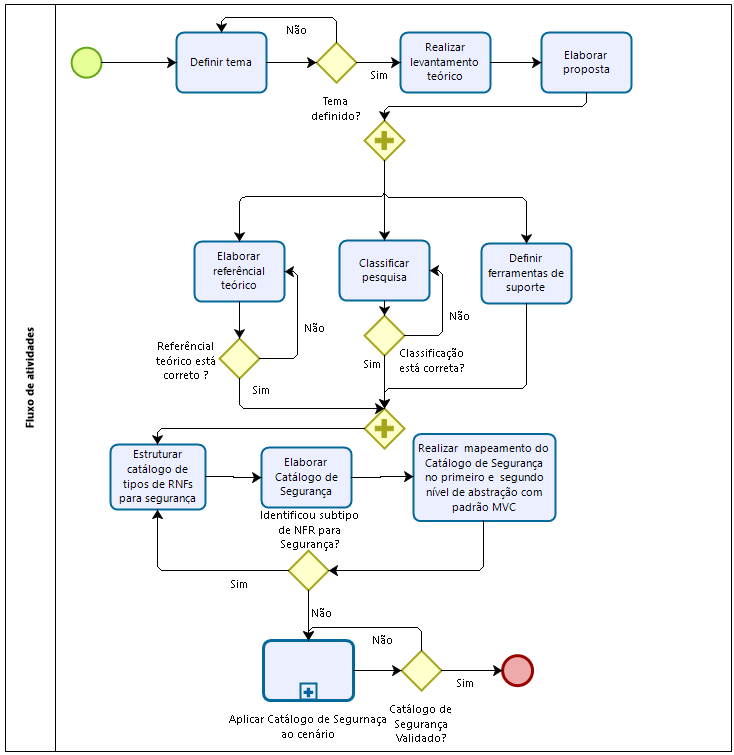
\includegraphics[keepaspectratio=true,scale=0.8]{figuras/fluxodeatividades.PNG}
	\caption{Atividades realizadas.}
	\label{fluxoDeExecuçãoTCC}
\end{figure}

Segue abaixo a descrição das atividades:

\begin{itemize}
	\item \textbf{Definir tema}: em conjunto com os professores orientadores dessa monografia, essa atividade teve como principal objetivo o refinamento sobre os conceitos teóricos referentes à área de interesse do autor;
	
	\item \textbf{Realizar levantamento teórico}: iniciou-se com base nos resultados obtidos na execução da atividade anterior, seguindo as orientações dos orientadores. Discutiu-se sobre os aspectos fundamentais do GORE, os \textit{frameworks} que se apoiam nos conceitos do GORE, os conceitos de Arquitetura de Software e os atributos de qualidade mais relevantes para o mercado e para a academia;
	
	\item \textbf{Elaborar proposta}: com o conhecimento das necessidades da área de atuação desse trabalho, iniciou-se a elaboração da proposta de pequisa, acordando que seria utilizado o NFR \textit{Framework}, bem como, que seria aplicado ao mercado, tomando Segurança como o principal atributo de qualidade;  
	
	\item \textbf{Elaborar referencial teórico}: foi realizada a redação dos conceitos teóricos a serem aplicados no desenvolvimento deste trabalho; 
	
	\item \textbf{Classificar pesquisa}: redação  da classificação da pesquisa em suas dimensões, sendo especificada quanto (i) à abordagem, (ii) à natureza, (iii) aos objetivos, e (iv) aos procedimentos técnicos;
	
	\item \textbf{Definir ferramentas de suporte}: definição e descrição das ferramentas utilizadas no desenvolvimento deste trabalho;
	
	\item \textbf{Estruturar catálogo de tipos de RNFs para Segurança}: com base nos conceitos de Segurança apresentados por Lawrence Chung, Brian A. Nixon, Eric Yu e John Mylopoulos, no  livro: \textit{NON-FUNCTIONAL REQUIREMENTS IN SOFTWARE ENGINEERING}, iniciou-se a elaboração do catálogo de tipos de RNFs para Segurança, expandindo o catálogo com base em definições de subtipos de RNFs;
	
	\item \textbf{Elaborar Catálogo de Segurança}: a partir do Catálogo de Segurança apresentado na Figura \ref{catalogoSegurancaChung}, iniciou-se o processo de identificação das metas flexíveis que podem ser suficientemente satisfeitas, orientando-se também pelo livro supracitado;
	
	\item \textbf{Realizar mapeamento do Catálogo de Segurança no primeiro e segundo nível de abstração com o padrão MVC}: iniciou-se a comparação das metas flexíveis que possuíam relação com o Padrão Arquitetural MVC, a fim de verificar se estas geram impactos, positivos ou negativos, na Segurança dos dados e da arquitetura. Durante a execução dessa atividade, caso ocorresse a identificação de outro subtipo de RNF para Segurança, a atividade “Estruturar catálogo de tipos para Segurança” seria realizada novamente e, consequentemente, as atividades seguintes, de acordo com a Figura \ref{fluxoDeExecuçãoTCC};
	
	\item \textbf{Aplicar Catálogo de Segurança ao cenário}: esta macroatividade respeitou a metodologia de desenvolvimento de software descrito na seção \ref{sec:metodologiaDeDesenvolvimentoDeSoftware}. Haja vista que, em cada ciclo foi definido um cenário com a descrição da persona, identificando, caso necessário, uma possível solução e realizando a aplicação do catálogo. Com isso, realizou-se o desenvolvimento do software, evidenciando a aplicação do catálogo e possibilitando a análise do quanto a Segurança do software pode ser satisfeita, e
	
	\item  \textbf{Realizar mapeamento em terceiro nível de abstração com padrão MVC}: esta atividade foi executada, em paralelo, com o processo de desenvolvimento das aplicações no cenário, onde permitiu aplicar o Catálogo de Segurança e realizar o detalhamento em terceiro nível de abstração, realizando o mapeamento das operacionalizações com as camadas do padrão arquitetural MVC. 
\end{itemize}


\subsection{Cronograma das Atividades}


O cronograma apresentado na Tabela \ref{cronogramaDoTrabalho}, organizado em meses, expõe como se deu a execução das atividades deste trabalho.

\begin{table}[h!]
	\tiny
	\label{cronogramaDoTrabalho}
	\caption{Cronograma de execução do trabalho.}
	\begin{tabular}{@{}lccccccccccccccc@{}}
		\toprule
		\multicolumn{1}{l|}{Ano} & \multicolumn{5}{c|}{\textbf{2017}} & \multicolumn{7}{c|}{\textbf{2018}} & \multicolumn{3}{c}{\textbf{2019}} \\ \midrule
		Atividade/Mês & \textbf{Ago} & \textbf{Set} & \textbf{Out} & \textbf{Nov} & \textbf{Dez} & \textbf{Jan} & \textbf{Fev} & - & \textbf{Ago} & \textbf{Set} & \textbf{Out} & \textbf{Dez} & \textbf{Jan} & \textbf{Fev} & \textbf{Mar} \\ \midrule
		Definir tema & \textbf{x} & \textbf{} & \textbf{} & \textbf{} & \textbf{} & \textbf{} & \textbf{} & - & \textbf{} & \textbf{} & \textbf{} & \textbf{} & \textbf{} & \textbf{} & \textbf{} \\ \midrule
		Elaborar proposta & \textbf{x} & \textbf{x} & \textbf{} & \textbf{} & \textbf{} & \textbf{} & \textbf{} & - & \textbf{} & \textbf{} & \textbf{} & \textbf{} & \textbf{} & \textbf{} & \textbf{} \\ \midrule
		\begin{tabular}[c]{@{}l@{}}Elaborar referencial\\  teórico\end{tabular} & \textbf{x} & \textbf{x} & \textbf{x} & \textbf{x} & \textbf{x} & \textbf{} & \textbf{} & - & \textbf{} & \textbf{} & \textbf{} & \textbf{} & \textbf{} & \textbf{} & \textbf{} \\ \midrule
		Classificar pesquisa & \textbf{} & \textbf{} & \textbf{x} & \textbf{x} & \textbf{x} & \textbf{} & \textbf{} & - & \textbf{} & \textbf{} & \textbf{} & \textbf{} & \textbf{} & \textbf{} & \textbf{} \\ \midrule
		\begin{tabular}[c]{@{}l@{}}Definir ferramentas\\ de suporte\end{tabular} & \textbf{} & \textbf{} & \textbf{x} & \textbf{x} & \textbf{x} & \textbf{} & \textbf{} & - & \textbf{} & \textbf{} & \textbf{} & \textbf{} & \textbf{} & \textbf{} & \textbf{} \\ \midrule
		\begin{tabular}[c]{@{}l@{}}Estruturar Catálogo\\  de Segurança\end{tabular} & \textbf{} & \textbf{} & \textbf{} & \textbf{} & \textbf{x} & \textbf{x} & \textbf{} & - & \textbf{} & \textbf{} & \textbf{} & \textbf{} & \textbf{} & \textbf{} & \textbf{} \\ \midrule
		\begin{tabular}[c]{@{}l@{}}Elaborar Catálogo\\ de Segurança\end{tabular} & \textbf{} & \textbf{} & \textbf{} & \textbf{} & \textbf{x} & \textbf{x} & \textbf{} & - & \textbf{} & \textbf{} & \textbf{} & \textbf{} & \textbf{} & \textbf{} & \textbf{} \\ \midrule
		\begin{tabular}[c]{@{}l@{}}Realizar Mapeamento\\ do Catálogo de\\  Segurança no \\ primeiro e segundo \\ nível de abstração\\ com padrão MVC.\end{tabular} & \textbf{} & \textbf{} & \textbf{} & \textbf{} & \textbf{} & \textbf{x} & \textbf{x} & - & \textbf{} & \textbf{} & \textbf{} & \textbf{} & \textbf{} & \textbf{} & \textbf{} \\ \midrule
		\begin{tabular}[c]{@{}l@{}}Aplicar Catálogo de\\ Segurança ao cenário\end{tabular} & \textbf{} & \textbf{} & \textbf{} & \textbf{} & \textbf{} & \textbf{} & \textbf{} & - & \textbf{x} & \textbf{x} & \textbf{x} & \textbf{x} & \textbf{x} & \textbf{x} & \textbf{} \\ \midrule
		\begin{tabular}[c]{@{}l@{}}Realizar mapeamento \\ em terceiro nível de \\ abstração\end{tabular} & \multicolumn{1}{l}{} & \multicolumn{1}{l}{} & \multicolumn{1}{l}{} & \multicolumn{1}{l}{} & \multicolumn{1}{l}{} & \multicolumn{1}{l}{} & \multicolumn{1}{l}{} & \multicolumn{1}{l}{-} & \textbf{x} & \textbf{x} & \textbf{x} & \textbf{x} & \textbf{x} & \textbf{x} & \textbf{x} \\ \bottomrule
	\end{tabular}
\end{table}

Observa-se que, foram utilizados, além do prazo base para a construção do Catálogo de Segurança, os meses de Janeiro/2018 e Fevereiro/2018. Isso ocorreu para melhor aprofundamento do tema, o qual demandou a leitura de vários materiais bibliográficos. Adicionalmente, as notações envolvidas nessa pesquisa são complexas, o que exige de um cuidado maior na escrita com o objetivo de promover uma melhor compreensão por parte dos interessados.

Com o Catálogo de Segurança concluído, se iniciou o ciclo de aplicação do mesmo em cada cenário. Essa aplicação ocorreu entre o período de Agosto de 2018 a Fevereiro de 2019, haja vista que, alguns cenários eram contextos reais. Dessa forma, somente em março de 2019, foi possível obter o mapeamento no terceiro nível de abstração.

\section*{Resumo do Capítulo}

Neste capítulo, foi detalhada na seção \ref{sec:classificacaoDaPesquisa}, a classificação de pesquisa de acordo com seus tipos, sendo estes: (i) abordagem, se tratando de uma pesquisa híbrida, a (ii) Natureza, caraterizada como uma pesquisa aplicada, o (ii) objetivo, caracterizado como uma pesquisa explicativa, e os (iv) procedimentos técnicos, caracterizados como uma pesquisa bibliográfica e a pesquisa-ação. Mais adiante, na seção \ref{sec:metodologiaDeDesenvolvimentoDeSoftware}, foi descrita a adaptação do \textit{Scrum} como metodologia de desenvolvimento de software e o Kanban para acompanhamento visual do andamento do desenvolvimento das aplicações nos cenários. Por fim, na seção \ref{sec:procedimentosMetodológicos}, o fluxo de atividades e o cronograma realizados na execução deste trabalho foram detalhados.


\chapter{Catálogo de Segurança}
\label{chap:proposta}

Neste Capítulo, é apresentada uma primeira versão do Catálogo de Segurança. Dado o volume de aspectos associados à Segurança, procurou-se focar nos tópicos mais relevantes, tendo como base a literatura. Dessa forma, o autor está ciente de que o Catalogo de Segurança não acorda todo e qualquer aspecto associado à Segurança. Mas, a intenção de demonstrar que um catálogo construído para especificar RNFs, utilizando uma notação adequada, mesmo que em alto nível de abstração, pode colaborar no entendimento das necessidades inerentes aos aspectos não-funcionais de um software, comumente colocados em segundo plano, ou apenas especificados em documentos, em linguagem natural. Esses documentos, como a Especificação Suplementar \cite{sommerville1997requirements}, carecem de uma notação que permita especificar os RNFs com toda a complexidade envolvida, ou seja, partindo de um alto nível de abstração, mas permitindo acordar operacionalizações, as quais de fato tornarão aquele RNF algo implementável, tratável a nível de código. Para a equipe de desenvolvedores, ter especificadas as operacionalizações pode promover soluções concretas para viabilizar a implementação de aspectos considerados abstratos. Para atingir esse objetivo, o Catálogo de Segurança foi especificado utilizando a notação do NFR \textit{Framework}, já comentada em capítulos anteriores. Essa notação propõe a elaboração de um grafo de interdependências entre os RNFs. Adicionalmente, deixa evidente as principais correlações entre esses RNFs, seus impactos e suas operacionalizações. Conforme justificado no Capítulo \ref{chap:introducao}, dada a relevância do RNF Segurança, têm-se que esse Catálogo de Segurança foca seus esforços na especificação desse RNF.

Para tornar mais compreensível o Catálogo de Segurança, optou-se por apresentá-lo, inicialmente, em dois níveis de abstração. Neste sentido, a seção \ref{sub:primeiroNivel} apresenta o primeiro nível de abstração. Nesse nível, são acordadas as metas flexíveis (representando os RNFs), seus impactos e suas operacionalizações. Utilizou-se a notação do NFR \textit{Framework}, com a elaboração de um grafo, SIG (\textit{Softgoal Interdependence Graph}). Na seção \ref{sub:segundoNivel}, é apresentado um mapeamento, procurando correlacionar as metas flexíveis e as camadas do Padrão Arquitetural MVC. Um terceiro nível de abstração também é mapeado e descritro no Capítulo \ref{chap:resultadosObtidos}, pois para alcançá-lo foi necessário realizar a aplicação do Catálogo de Segurança em cenários. Sendo este, o terceiro nível de abstração entre as operacionalizações e as camadas do Padrão Arquitetural MVC, devido ao fato de envolver aspectos em um nível mais baixo de abstração (implementando de fato as operacionalizações nas camadas \textit{Model-View-Controller}).

\section{O Catálogo de Segurança}

Essa primeira versão do Catálogo de Segurança procura promover, aos especialistas, uma maior compreensão quanto às diferentes necessidades se tratando de Segurança. O Catálogo de Segurança acorda os principais conceitos associados à Segurança, tomando como base o levantamento bibliográfico realizado nessa pesquisa.

Conforme colocado anteriormente, neste capítulo, o Catálogo de Segurança será apresentado em dois níveis de abstração. O primeiro nível, descrito na seção \ref{sub:primeiroNivel}, procura apresentar as metas flexíveis - ou RNFs - associadas à Segurança. O grafo especifica ainda as correlações e os impactos entre essas metas flexíveis, bem como as operacionalizações (no nível mais baixo do grafo). O segundo nível é apresentado na seção \ref{sub:segundoNivel}, como um mapeamento entre as metas flexíveis e as camadas do Padrão Arquitetural MVC.

\subsection{Primeiro Nível de Abstração}
\label{sub:primeiroNivel}

O primeiro nível de abstração apresenta as metas flexíveis mais genéricas de Segurança de software, apoiando-se, principalmente, na definição de Chung. Essa definição baseia-se em Confidencialidade, Integridade e Disponibilidade. Adicionalmente, essa abstração também se apoia na definição de Segurança da Informação apresentada na ISO 27001. 

\begin{citacao}
	"Segurança da informação: preservação da \textbf{confidencialidade}, \textbf{integridade} e \textbf{disponibilidade} da informação; adicionalmente, outras propriedades, tais como \textbf{autenticidade}, \textbf{responsabilidade}, não repúdio e \textbf{confiabilidade}, podem também estar envolvidas." \cite[p. 2]{documentation2005information}
\end{citacao}


As metas flexíveis foram definidas de acordo com sua relação com Segurança. Observa-se que foram acrescentados, à notação do SIG, alguns valores representados como referências. A intenção é permitir a rastreabilidade de cada aspecto representado no grafo com sua respectiva fonte ou referência teórica. Esse rastreamento permite ao leitor: (i) ter a comprovação de que a especificação do catálogo foi de fato apoiada na literatura, e (ii) aprofundar seus conhecimentos e, caso assim o desejar, consultar as referências para maior esclarecimento sobre cada especificação sugerida no Catálogo de Segurança. A Tabela \ref{indicesDeReferencia} apresenta os identificadores para a rastreabilidade da referência teórica de uma meta flexível no SIG da Figura \ref{DetalhamentoPrimeiroNivel}. 

\pagebreak

\begin{table}[h!]
	\centering
	\caption{Índices de rastreabilidade.}
	\label{indicesDeReferencia}
	\begin{tabular}{@{}cc@{}}
		\toprule
		\textbf{Identificador} & \textbf{Referência} \\ \midrule
		{[}1{]} & \cite{chung2012non} \\ 
		{[}2{]} & \cite{benitti2015taxonomia} \\
		{[}3{]} & \cite{documentation2005information} \\
		{[}4{]} & \cite{affleck2012supporting} \\
		{[}5{]} & \cite{buschmann1996system}
		\\ \bottomrule
	\end{tabular}
\end{table} 


\begin{figure}[h!]
	\centering
	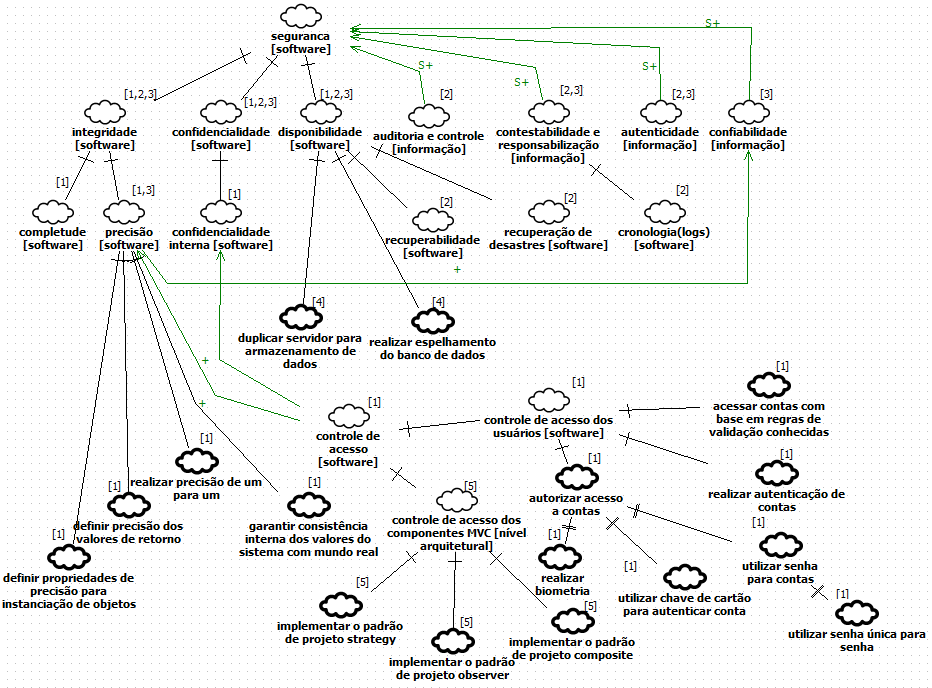
\includegraphics[keepaspectratio=true,scale=0.7]{figuras/CatalogoDeSeguranca.PNG}
	\caption{Catálogo de Segurança.}
	\label{DetalhamentoPrimeiroNivel}
\end{figure}


As definições das metas flexíveis e operacionalizações são: 

\begin{itemize}
	
	\item \textbf{integridade:} proteção contra qualquer tipo de atualização e/ou adulteração não autorizada. Definida na seção \ref{sec:seguranca};
	
	\begin{itemize}
		
		\item \textbf{precisão:} pode ser entendida como qualquer atributo semântico que fundamenta uma informação. Definida na seção \ref{sec:seguranca};
		
		\begin{itemize}
			
			\item \textbf{\textit{definir propriedades de precisão para instanciação de objetos:}} garantir que objetos sejam instanciados da maneira correta. Definida na seção \ref{sec:seguranca};
			
			\item \textbf{\textit{definir precisão dos valores de retorno:}} garantir que os valores retornados pelas operações possuam a precisão pré-estabelecida. Definida na seção \ref{sec:seguranca};
			
			\item \textbf{\textit{realizar precisão de um para um:}} garantir que um único objeto esteja ligado a uma única entidade do domínio. Definida na seção \ref{sec:seguranca};
			
			\item \textbf{\textit{garantir consistência interna dos valores do sistema com mundo real:}} garantir que os valores do mundo real sejam correspondentes aos valores do sistema. Definida na seção \ref{sec:seguranca};
			
			\item \textbf{controle de acesso:} nível mais genérico para autorização de acesso definido por \cite{chung2012non}, trata-se das especificações de controle de acesso do software; 
			
			\begin{itemize}
				
				\item \textbf{controle de acesso dos usuários:} controle de acesso de usuários no software \cite{chung2012non}. Para ser satisfeita, depende de um conjunto de operacionalizações: \textbf{\textit{autorizar acesso a contas}}, \textbf{\textit{acessar contas com base em regras de validação conhecidas}} e \textbf{\textit{realizar autenticação de contas}};
				
				\item \textbf{controle de acesso dos componentes MVC:} trata-se das restrições arquiteturais impostas pelo padrão arquitetural MVC para que as relações internas entre os componentes sejam realizadas \cite{buschmann1996system}. Para que isso ocorra, devem ser implementados três \textit{design patterns}, que são abstraídos no catálogo de Segurança como operacionalizações, sendo elas: (i) \textbf{\textit{implementar o padrão de projeto strategy}}, (ii) \textbf{\textit{implementar o padrão de projeto observer}} e (iii) \textbf{\textit{implementar o padrão de projeto composite}};
				
			\end{itemize}
						
		\end{itemize}
		
		\item \textbf{completude:} garantia que o RNF esteja o mais completo possível. Definida na seção \ref{sec:seguranca};
	\end{itemize}
	
	\item \textbf{confidencialidade:} proteção da informação para evitar que as informações armazenadas ou transmitidas não sejam vistas ou interpretadas por terceiros, sendo somente o usuário principal e o destinatário. Definida na seção \ref{sec:seguranca};
	
	\begin{itemize}
		
		\item \textbf{confidencialidade interna:} proteção da informação que o acesso deve ser evitado por um público externo. Definida na seção \ref{sec:seguranca};
		
	\end{itemize}
	 
	 \item \textbf{disponibilidade:} proteção contra a interrupção do serviço, no momento em que o usuário estiver utilizando a aplicação. Definida na seção \ref{sec:seguranca};
	 
	 \begin{itemize}
	 		
	 		\item \textbf{recuperabilidade:} intervalo de tempo que o software deverá estar disponível após uma falha \cite{benitti2015taxonomia};
	 	
	 		\item \textbf{recuperação de desastres:} políticas e procedimentos aplicados na recuperação de ``desastres`` induzidos no software por usuário ou softwares de terceiros \cite{benitti2015taxonomia};
	 		
	 		\item \textbf{\textit{duplicar servidor para armazenamento de dados:}} promove menor chance de tempo onde ocorra a inatividade dos dados. Com a utilização de dois ou mais servidores em funcionamento, a disponibilidade dos dados do software é maior \cite{date2004introduccao}\cite{affleck2012supporting};   
	 		
	 		\item \textbf{\textit{realizar espelhamento do banco de dados:}} compreende-se como duas cópias de um único banco de dados que geralmente reside em máquinas diferentes \cite{date2004introduccao}\cite{affleck2012supporting}; 
	 		
	 \end{itemize}
 
 	\item \textbf{auditoria e controle:} especificação dos aspectos que devem ser contemplados para proporcionar a auditoria e o controle \cite{benitti2015taxonomia}; 
 	
 	\item  \textbf{contestabilidade e responsabilização:} capacidade do software em quantificar as ações e os eventos, com intuito de comprovar sua ocorrência \cite{benitti2015taxonomia}; 
 	
 	\begin{itemize}
 		
 		\item \textbf{cronologia(logs):} registro de alterações no software \cite{benitti2015taxonomia};
 		
 	\end{itemize}
 	
 	\item \textbf{autenticidade:} capacidade do software em identificar que um objeto ou recurso é o que ele realmente declara ser \cite{benitti2015taxonomia}, e
 	
 	\item \textbf{confiabilidade:} capacidade do software em realizar e manter seu funcionamento quando submetido em circunstâncias de rotina \cite{benitti2015taxonomia}. 
 	
\end{itemize}

\subsection{Segundo Nível de Abstração}
\label{sub:segundoNivel}

O segundo nível de abstração procura correlacionar as metas flexíveis mais genéricas e as camadas do Padrão Arquitetural MVC. As Tabelas \ref{mapeamento1} e \ref{mapeamento2} apresentam esse mapeamento, considerando diferentes níveis de satisfação para cada meta flexível.


\begin{table}[h!]
	\centering
	\caption{Mapeamento das metas flexíveis com as camadas do MVC - Parte 1.}
	\label{mapeamento1}
	\tiny
	\begin{tabular}{@{}cccp{5cm}cc@{}}
		\toprule
		\multicolumn{1}{l}{\textbf{id}} & \multicolumn{1}{l}{\textbf{Meta flexível}} & \multicolumn{1}{l}{\textbf{\begin{tabular}[c]{@{}l@{}}Nível de\\ satisfação\end{tabular}}} & \multicolumn{1}{l}{\textbf{Descrição}} & \multicolumn{1}{l}{\textbf{Referência}} & \multicolumn{1}{l}{\textbf{Camada}} \\ \midrule
		1 & \begin{tabular}[c]{@{}c@{}}“precisão\\ {[}software{]}”\end{tabular} & \begin{tabular}[c]{@{}c@{}}Suficientemente\\ Satisfeita\end{tabular} & Garante que um ou mais objetos estejam ligados a uma única entidade do domínio. Além disso, impacta diretamente a \textit{Model} pois é a camada que representa os aspectos do domínio da aplicação.
		
		
		- Atributo de precisão: precisão de um para um. & \begin{tabular}[c]{@{}c@{}}\cite{chung2012non}\\ \cite{buschmann1996system}\end{tabular} & \textit{model} \\
		
		\rowcolor[HTML]{C0C0C0} 2 & \begin{tabular}[c]{@{}c@{}}“precisão\\ {[}software{]}”\end{tabular} & \begin{tabular}[c]{@{}c@{}}Suficientemente\\ Satisfeita\end{tabular} & Garante que os objetos sejam instanciados da maneira correta dentro da \textit{model}.
		
		- Atributo de precisão: Propriedade da precisão. & \begin{tabular}[c]{@{}c@{}}\cite{chung2012non}\\ \cite{buschmann1996system}\end{tabular} & \textit{Model} \\
		
		3 & \begin{tabular}[c]{@{}c@{}}“autenticidade\\ {[}informação{]}”\end{tabular} & \begin{tabular}[c]{@{}c@{}}Satisfeita\\ Suficientemente\end{tabular} & A utilização de \textit{triggers} em banco de dados promove a autenticidade e a verificação da integridade do dado. Além disso, pode ser utilizada para realização de auditoria em tabelas. &  &  \\
		\cellcolor[HTML]{C0C0C0}4 & \cellcolor[HTML]{C0C0C0}\begin{tabular}[c]{@{}c@{}}“integridade\\ {[}software{]}”\end{tabular} & \cellcolor[HTML]{C0C0C0}\begin{tabular}[c]{@{}c@{}}Satisfeita\\ Suficientemente\end{tabular} & \cellcolor[HTML]{FFFFFF} &  &  \\
		5 & \begin{tabular}[c]{@{}c@{}}“auditoria e\\  controle\\ {[}informação{]}”\end{tabular} & \begin{tabular}[c]{@{}c@{}}Satisfeita\\ Suficientemente\end{tabular} & \multicolumn{1}{l}{} & \multirow{-3}{*}{\cite{date2004introduccao}} & \multirow{-3}{*}{\begin{tabular}[c]{@{}c@{}}Banco \\ de Dados\end{tabular}} \\
		
		\rowcolor[HTML]{C0C0C0} 
		\multicolumn{1}{l}{\cellcolor[HTML]{C0C0C0}6} & \begin{tabular}[c]{@{}c@{}}“controle\\  de acesso usuário\\ {[}software{]}”\end{tabular} & \begin{tabular}[c]{@{}c@{}}Parcialmente\\ Satisfeita\end{tabular} & O método de autenticação dos dados retorna a instância do usuário, quando a senha está correta. Esse aspecto é implementado diretamente na \textit{Controller}. Entretanto, possui clara relação com a \textit{View} e com a base de dados. Considera-se “Parcialmente Satisfeita”, pois há dependência com a operacionalização “Autorizar Acesso a Contas", a qual contribui para a satisfação dessa meta flexível “controle de acesso {[}software{]}”. & \cite{fuentes2014ruby} & \textit{Controller} \\
		
		\multicolumn{1}{l}{7} & \begin{tabular}[c]{@{}c@{}}“confiabilidade\\ {[}informação{]}”\end{tabular} & \begin{tabular}[c]{@{}c@{}}Suficientemente\\ Satisfeita\end{tabular} & Garante que o conjunto de dados a serem armazenados na base de dados estejam relativamente fidedignos. Usa-se “relativamente”, pois não há como garantir algo pleno, se tratando de critérios tão abstratos. Nesse caso, “relativamente” sugere que seja o mais fidedigno/confiável possível”. & \cite{fuentes2014ruby} & \textit{View} \\ 
		
		\rowcolor[HTML]{C0C0C0} 
		8 & \begin{tabular}[c]{@{}c@{}}“controle de \\ acesso dos \\ componentes \\ MVC\\ {[}nível arquitetural{]}”\end{tabular} & \begin{tabular}[c]{@{}c@{}}Parcialmente\\ Satisfeita\end{tabular} & Garante que os componentes da \textit{View}, os quais dependem de outros componentes que se encontram em outras camadas do modelo MVC, reconheçam a necessidade de atualizar as telas, adequando-as às demandas encaminhadas via \textit{Controller} (por exemplo) e em compatibilidade com os dados especificados na \textit{Model}. Considera-se “parcialmente satisfeita”, pois há dependência com a implementação do padrão de projeto estrutural \textit{Composite}. A implementação é sugerida como operacionalização que contribue para satisfação dessa meta flexível, “controle de acesso dos componentes MVC {[}nível arquitetural{]}.” & \begin{tabular}[c]{@{}c@{}}\cite{baptistella2011abordando} \\ \cite{buschmann1996system}\end{tabular} & \textit{View} \\
		
		\bottomrule
	\end{tabular}
\end{table}

\begin{table}[p]
	\centering
	\caption{Mapeamento das metas flexíveis com as camadas do MVC - Parte 2.}
	\label{mapeamento2}
	\tiny
	\begin{tabular}{@{}cccp{5cm}cc@{}}
		\hline
		\multicolumn{1}{l}{\textbf{id}} & \multicolumn{1}{l}{\textbf{Meta flexível}} & \multicolumn{1}{l}{\textbf{\begin{tabular}[c]{@{}l@{}}Nível de\\ satisfação\end{tabular}}} & \multicolumn{1}{l}{\textbf{Descrição}} & \multicolumn{1}{l}{\textbf{Referência}} & \multicolumn{1}{l}{\textbf{Camada}} \\ \hline
		\rowcolor[HTML]{C0C0C0} 
		8 & \begin{tabular}[c]{@{}c@{}}“controle de \\ acesso dos \\ componentes \\ MVC\\ {[}nível arquitetural{]}”\end{tabular} & \begin{tabular}[c]{@{}c@{}}Parcialmente\\ Satisfeita\end{tabular} & Garante que os componentes da \textit{View}, os quais dependem de outros componentes que se encontram em outras camadas do modelo MVC, reconheçam a necessidade de atualizar as telas, adequando-as às demandas encaminhadas via \textit{Controller} (por exemplo) e em compatibilidade com os dados especificados na \textit{Model}. Considera-se “Parcialmente Satisfeita”, pois há dependência com a implementação do padrão de projeto estrutural \textit{Composite}. A implementação é sugerida como operacionalização que contribue para satisfação dessa meta flexível, “controle de acesso dos componentes MVC {[}nível arquitetural{]}.” & \begin{tabular}[c]{@{}c@{}}\cite{baptistella2011abordando} \\ \cite{buschmann1996system}\end{tabular} & \textit{View} \\
		9 & \begin{tabular}[c]{@{}c@{}}“controle de\\ acesso dos \\ componentes\\ MVC\\ {[}nível arquitetural{]}”\end{tabular} & \begin{tabular}[c]{@{}c@{}}Parcialmente\\ Satisfeita\end{tabular} & Garante que a \textit{Model} esteja menos acoplada em relação à \textit{View} e à \textit{Controller}, viabilizando essa relação através de boas práticas da Engenharia de Software. Uma dessas práticas é sugerida como operacionalização na Figura \ref{DetalhamentoPrimeiroNivel}, apoiando-se no uso de Padrões de Projeto. Considera-se parcialmente satisfeita, pois há dependência com a implementação do padrão de projeto comportamental \textit{Observer}, por exemplo. Essa implementação é sugerida como uma operacionalização possível em atendimento a essa demanda e contribui para a satisfação dessa meta flexível, “controle de acesso dos componentes MVC{[}nível arquitetural{]}”. & \begin{tabular}[c]{@{}c@{}}\cite{baptistella2011abordando} \\ \cite{buschmann1996system}\end{tabular} & \textit{Model} \\
		\rowcolor[HTML]{C0C0C0} 
		10 & \begin{tabular}[c]{@{}c@{}}“controle de\\ acesso dos \\ componentes\\ MVC\\ {[}nível arquitetural{]}”\end{tabular} & \begin{tabular}[c]{@{}c@{}}Parcialmente\\ Satisfeita\end{tabular} & Garante menor acoplamento entre as camadas MVC. Sugere-se que tal aspecto seja apoiado no uso de Padrões de Projeto. Portanto, acredita-se que o padrão de projeto \textit{Strategy}, implementado na \textit{Controller}, permita menor acoplamento entre \textit{View} e \textit{Model}, sendo, de fato, responsabilidade da \textit{Controller} intermediar essa relação utilizando decisões estratégicas. Vale ressaltar que, com o uso desse padrão de projeto decisões podem ser tomadas em tempo de execução, alterando o comportamento do software em função das demandas conhecidas dinamicamente. Dessa forma, a tendência é de maior cumprimento de boas práticas já acordadas no padrão arquitetural MVC. Considera-se parcialmente satisfeita, pois há dependência com a implementação do padrão de projeto comportamental \textit{Strategy}, por exemplo. Essa implementação é sugerida como uma operacionalização possível em atendimento a essa demanda, e contribui para a satisfação dessa meta flexível, “controle de acesso dos componentes MVC{[}nível arquitetural{]}”. & \begin{tabular}[c]{@{}c@{}}\cite{baptistella2011abordando} \\ \cite{buschmann1996system}\end{tabular} & \textit{Controller} \\ \hline
	\end{tabular}
\end{table}

\pagebreak
\pagebreak

\section*{Resumo do Capítulo}

Neste capítulo, foi apresentada uma primeira versão do Catálogo de Segurança proposto nessa pesquisa. Adicionalmente, foram apontados os principais impactos e as contribuições das informações do Catálogo de Segurança em relação às camadas do Padrão Arquitetural MVC. Ressalta-se que, o Catálogo foi especificado apoiando-se na literatura, conforme pode ser observado considerando a rastreabilidade, apresentada na seção \ref{sub:primeiroNivel} evidenciando o primeiro nível de abstração. Nesse nível, foram descritas as metas flexíveis associadas à Segurança. O Catálogo de Segurança especificou as correlações e os impactos entre as metas flexíveis, bem como as operacionalizações.. O segundo nível de abstração foi apresentado na seção \ref{sub:segundoNivel}, demonstrando o mapeamento entre as metas flexíveis e as camadas do Padrão Arquitetural MVC.

Por fim, cabe mencionar que o Catálogo de Segurança ainda possui mais um nível de abstração, o qual será demonstrado no Capítulo \ref{chap:resultadosObtidos}, pois só foi possível mapear a correlação entre as operacionalizações e as camadas MVC
com a aplicação em cenários. Tal prática permitiu apresentar como os critérios de qualidade podem ser suficientemente tratados e satisfeitos a nível de código.

\chapter{Resultados Obtidos}
\label{chap:resultadosObtidos}

Neste capítulo são apresentadas as primeiras aplicações do Catálogo de Segurança e o mapeamento no terceiro nível de abstração (entre operacionalizações e as camadas do Padrão Arquitetural MVC). Para isso, foi utilizado o conceito de \textit{personas}, apresentado na seção \ref{sec:personas}, com o objetivo de demonstrar os cenários nos quais o catálogo pode ser aplicável. Portanto, realizou-se a simulação de cinco cenários para validar a aplicação do Catálogo de Segurança. 

O capítulo é dividido, inicialmente, pelos cenários contextualizados dentro de cada persona. Os cenários têm a descrição da persona, identificação da possível solução (Quando necessário descrever para o cenário) e a aplicação do catálogo. Ao final do capítulo é apresentada a primeira visão da aplicação do Catálogo de Segurança.  


\section{Cenário 1}
\label{subsec:persona1}

Heleno, 24 anos, Engenheiro de Requisitos, assumiu a função de elicitar os requisitos não funcionais para um novo projeto na empresa em que trabalha. O projeto será desenvolvido em \textit{Rails} e seu chefe solicitou perfis diferentes de membro e administrador. O sistema solicitado pelo chefe deve, principalmente, ser seguro para autenticação do usuário, bem como, com capacidade de redefinição da senha, monitoramento da quantidade de entradas e, por fim, validação do email do mesmo.

\begin{itemize}
	\item O problema: mapear os métodos de autenticação relevantes para autenticar o usuário; 
	\item Objetivo: verificar o nível de satisfação de segurança da aplicação, e
	\item Desafio: analisar os impactos entre os requisitos não funcionais para autenticar os usuários.
\end{itemize}


\subsection{Identificar possível solução}

O problema principal do usuário é a realização da autenticação do mesmo. O primeiro passo a ser adotado é identificar qual \textit{gem} é a mais adequada. Segundo o \textit{The Ruby Toolbox}, na categoria \textit{Rails Authentication}, o ranking de popularidade das três \textit{gems} mais utilizadas para autenticação é \cite{rubytoolbox}:

\begin{enumerate}
	\item devise: 38.982.741 downloads
	\item omniauth: 23.524.509 downloads
	\item doorkeeper: 7.091.328 downloads
\end{enumerate}

Portanto, a \textit{gem} selecionada por Heleno para ser aplicada ao projeto é a \textit{devise}, pois além da sua posição no ranking, é a \textit{gem} mais recomendada pela comunidade \textit{Rails}. As vantagens da utilização do \textit{devise} são  (i) solução baseada no padrão arquitetural MVC, (ii) criação e a utilização de vários perfis de usuários conectados ao mesmo tempo, e (iii) utilização somente daquilo que é necessário, baseando-se no conceito de modularidade. Essa \textit{gem} possui 10 módulos \cite{gemdevise}: 

\begin{enumerate}
	\item \textit{Database Authenticatable}: \textit{hashes} que armazenam a senha no banco de dados para serem validadas durante o \textit{login}. A autenticação pode ser realizada via método POST ou HTTP \textit{basic authentication}; 
	
	\item \textit{Omniauthable}: suporte adicional ao \textit{omniauth};
	
	\item \textit{Confirmable}: envio automático de email para confirmação da conta e verificação da confirmação da conta durante o \textit{login};
	
	\item \textit{Recoverable}: envia instruções de redefinição de senha para o usuário e redefine a senha do usuário;
	
	\item \textit{Registerable}: permite a inscrição de usuários por meio do processo de registros, permitindo a edição e a remoção de suas contas;
	
	\item \textit{Rememberable}: gerenciador de \textit{token} para notificar o usuário da existência de \textit{cookie} salvo;
	
	\item \textit{Trackable}: contador de entradas, mantendo o registro de data, hora e endereço de IP;
	
	\item \textit{Timeoutable}: expira as sessões inativas em um período de tempo especificado;
	
	\item \textit{Validatable}: validações de email e senha, e
	 
	\item \textit{Lockable}: bloqueia a conta após exceder o número de tentativas especificado. Portanto, o desbloqueio pode ocorrer via email ou após um período de tempo. 
\end{enumerate}

\subsection{Aplicação do Catálogo de Segurança}

A partir do uso do Catálogo de Segurança, foi possível realizar o mapeamento dos módulos apresentados anteriormente. Então, modelou-se a \textit{gem devise} e seus respectivos métodos como operacionalizações no catálogo. 

\pagebreak

\begin{figure}[h!]
	\centering
	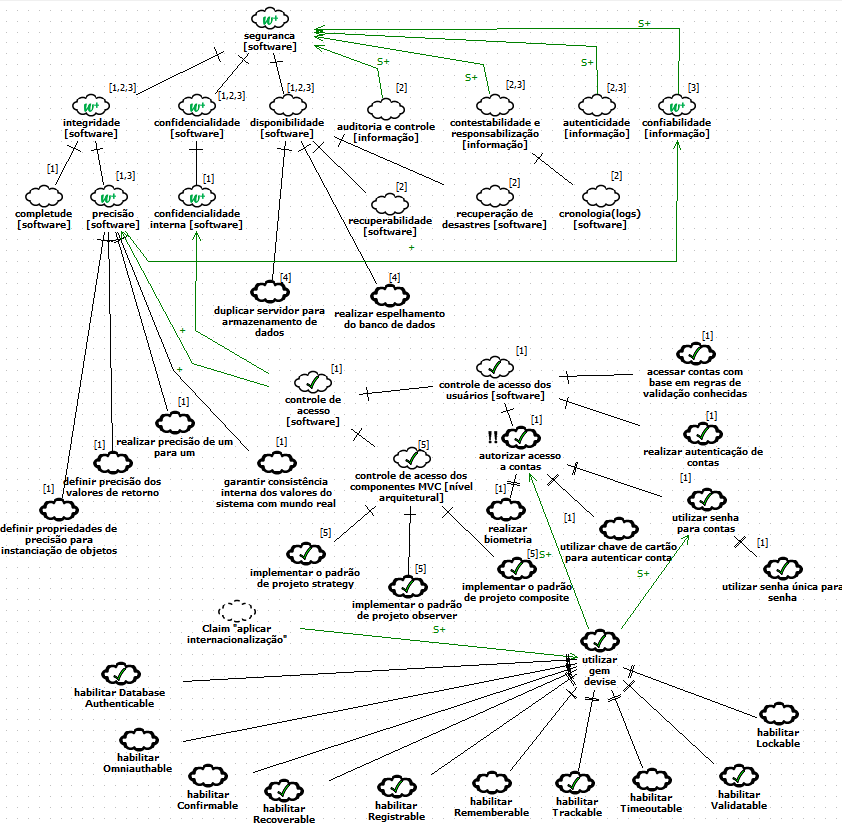
\includegraphics[keepaspectratio=true,scale=0.7]{figuras/catalogoPersona1.PNG}
	\caption{Operacionalizações para autenticação de usuário utilizando a \textit{gem devise}.}
	\label{catalogoPersona1}
\end{figure}


O Catálogo de Segurança aplicado no cenário 1 é apresentado na Figura \ref{catalogoPersona1}, na qual as operacionalizações foram incrementadas ao catálogo inicial. Respeitando os módulos da \textit{gem devise}, a operacionalização  “autorizar acesso a contas” passou a possuir alto grau de prioridade devido ao cenário, pois esta é uma das operacionalizações que impactam diretamente a solução para o problema. 

É possível, então, utilizando a notação do NFR \textit{Framework}, realizar a modelagem da \textit{gem devise} como uma operacionalização, representando a existência de alguma contribuição positiva (SOME+) com as operacionalizações  “autorizar acesso a contar” e “utilizar senha para contas”.
 
As operacionalizações filhas de “utilizar \textit{gem devise}” e que atendem as necessidades da persona descrita no cenário 1 são:

\begin{itemize}
	\item “habilitar \textit{Database Authenticatable}”: é um dos requisitos mínimos para que ocorra a persistência da senha no banco de dados;
	\item “habilitar \textit{Recoverable}”: capacidade de redefinir a senha do usuário;
	\item “habilitar \textit{Registrable}”: é um dos requisitos mínimos e que permite a inscrição de usuários; 
	\item “habilitar \textit{Trackable}”: monitorar a quantidade de entradas do usuário, e 
	\item “habilitar \textit{Validatable}”: validar conta via email do usuário. 
\end{itemize}

Portanto, ao habilitar os módulos da \textit{gem devise} dentro da camada \textit{model}, nas classes \textit{Admins} e \textit{Members}, as operacionalizações são satisfeitas. Podemos então, verificar qual nível de satisfação da segurança do software pode ser alcançado com a utilização da \textit{gem devise}. 

O trecho de código abaixo apresenta como pode ser os módulos podem ser habilitados.  
 
\begin{lstlisting} 
class Admins < ApplicationRecord
devise :database_authenticatable, :registerable,
:recoverable, :rememberable, :trackable, :validatable
end 
\end{lstlisting} 

A implementação dos padrões de projeto \textit{strategy}, \textit{observer} e \textit{composite} já estão suficientemente satisfeitos, pois a aplicação é desenvolvida com o \textit{framework rails} que obedece o padrão MVC e a \textit{gem} que está sendo utilizada também percorre todas as camadas. 

\section{Cenário 2}
\label{subsec:persona2}

Pedro, 23 anos, Engenheiro de Software, trabalha em empresa privada e possui a necessidade de desenvolver o sistema da ouvidoria da instituição. Tal sistema deverá ser desenvolvido em plataforma web para atender os processos de manifestação (denúncia, reclamação, solicitação, sugestão e elogio) realizados pela ouvidoria. Esse tipo de informação deve ser estritamente confidencial, podendo ou não, o manifestante ser anônimo.  

\subsection{Identificar possível solução}

Uma possível solução é gerar um número de protocolo, durante o registro da manifestação, para que possa ser realizado o acompanhamento. Tal número será utilizado tanto para a manifestação anônima, quanto para a manifestação formal. O manifestante poderá acompanhar o status de sua manifestação através da visão de acompanhamento, na qual ficarão registradas as respostas dadas pela ouvidora.

A Ouvidora, no caso, acessará o sistema de forma diferente, utilizando a área administrativa do sistema através da autenticação de usuário. Ao fazer isso, a mesma estará apta a visualizar todas as manifestações e selecionar a desejada, para que seja possível a redação da resposta para o manifestante.  

\subsection{Aplicação do Catálogo de Segurança}

\begin{figure}[h!]
	\centering
	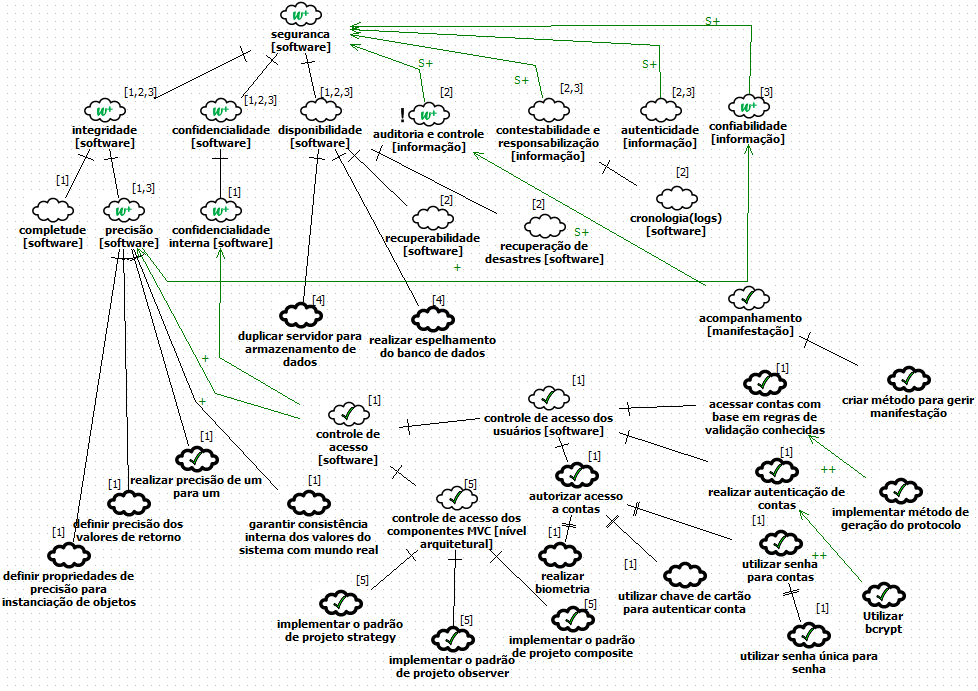
\includegraphics[keepaspectratio=true,scale=0.6]{figuras/catalogoPersona2.PNG}
	\caption{Catálogo de segurança aplicado ao sistema de ouvidoria.}
	\label{catalogoPersona2}
\end{figure}



Na aplicação do Catálogo de Segurança da figura \ref{catalogoPersona2}, surgiu a necessidade de focar em  “auditoria e controle”, pois o cenário demandava  o acompanhamento das manifestações pelos ouvidores. Com isso, foi expandido no Catálogo de Segurança uma nova meta flexível “Realizar acompanhamento das manifestações” e uma operacionalização “Criar método para gerir manifestação”. A operacionalização é definida pelos métodos implementados na \textit{controller - ManagerManifestationsController}. Portanto, a meta flexível “auditoria e controle” é suficientemente satisfeita para este contexto.

Para que a meta flexível “controle de acesso dos usuários” seja suficientemente satisfeita, as três operacionalizações que estão no nível mais baixo no Catálogo de Segurança também serão, sendo elas: (i) “implementar método de geração do protocolo”: trata-se de um método para gerar os números de protocolos com caracteres (de “a” à “z”), (de “A” à “Z”) e (de “0” à “9”) composto por 10 dígitos; (ii) “utilizar senha única para senha”: para cada usuário administrador/ouvidor cadastrado no sistema é gerada uma única senha para autenticação; e (iii) “utilizar bcrypt”: refere-se a uma \textit{gem} que utiliza algoritmo de \textit{hashing} criptográfico trata um trecho do dado para gerar um \textit{hash}. Considerando que, ao gerar uma senha dessa maneira, trata-se da execução de um processo não reversível, visto que não há como retornar da \textit{hash} para a senha \cite{brcypt}.

A operacionalização “realizar precisão de um para um” é suficientemente satisfeita, pois para cada manifestação ocasionada por determinado evento de manifestação do mundo real existirá uma única manifestação no sistema.

Diante do exposto, observa-se que a segurança do software é parcialmente satisfeita devido a satisfação parcial da integridade e da confidencialidade do mesmo.

\section{Cenário 3}
\label{subsec:persona3}

Milena, 22 anos, Engenheira de Software, possuindo várias atividades no seu dia-a-dia, sentiu a necessidade de organizá-las e para isso, considerando as suas habilidades, decidiu escrever um programa com o objetivo de obter melhor controle sobre as mesmas. Esse programa permite a inserção da atividade com sua descrição, a data de início, a previsão de conclusão e seu status. Consequentemente, Milena optou por fazer seu sistema em \textit{Rails} e decidiu verificar as relações entre as camadas do sistema com o foco em segurança.

\begin{itemize}
	\item O problema: desorganização das atividades diárias;
	\item Objetivo: desenvolvimento de sistema para auxiliar na organização das atividades, e
	\item Desafio: verificar as relações entre as camadas do sistema com foco em segurança.
\end{itemize}

\subsubsection{Aplicação do Catálogo de Segurança}

Na descrição da persona, houve a necessidade de vincular cada atividade do mundo real com ao menos uma entidade no sistema. Para isso utilizou-se o comando \textit{scaffold} do \textit{Rails}. Tal comando gera a estrutura de arquivos de acordo com o padrão MVC, gerando o \textit{model}, o \textit{controller}, os \textit{views} necessários \cite{railscommunity}. 

\begin{figure}[h!]
	\centering
	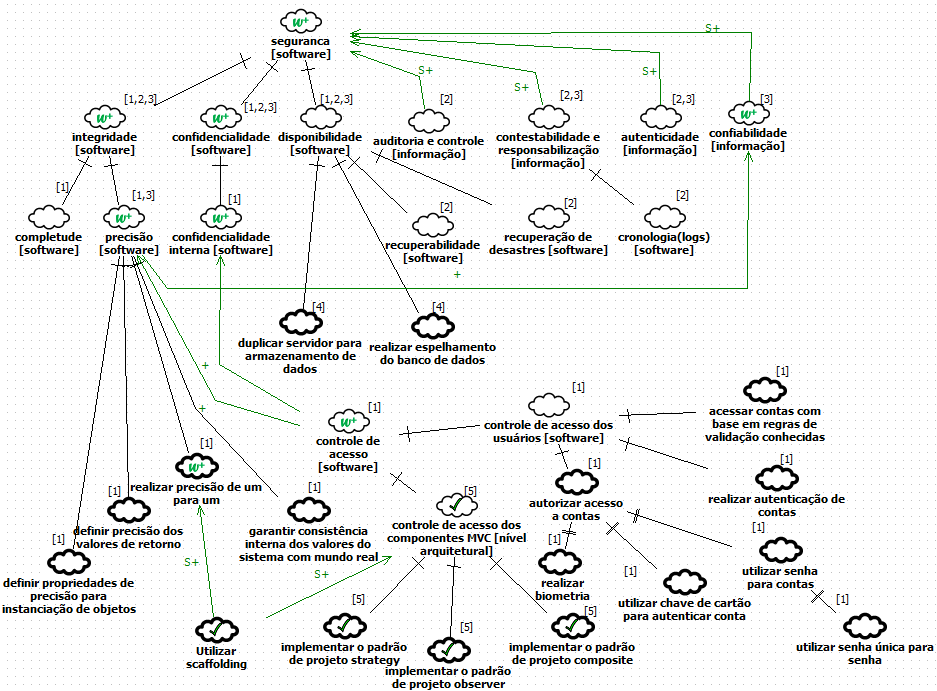
\includegraphics[keepaspectratio=true,scale=0.7]{figuras/catalogoPersona3.PNG}
	\caption{O \textit{scaffolding} do \textit{Rails} no Catálogo de Segurança.}
	\label{catalogoPersona3}
\end{figure}

\section{Cenário 4}
\label{subsec:persona4}

Gustavo, 23 anos, Engenheiro de Requisitos de empresa privada, possui a demanda de analisar os requisitos do sistema de solicitação de documentos digitais via plataforma web. Tal sistema possui arquitetura MVC e está em constante evolução. Assim sendo, seu chefe solicitou que o mesmo fizesse uma análise dos RNFs com foco na segurança do sistema, devido a emissão de documentos com assinatura digital. 

\subsection{Identificar possível solução}

A aplicação do Catálogo de Segurança pode ser uma das maneiras de demonstrar a relação entre os RNFs do sistema, principalmente, quando o RNF que está em foco é segurança.

\pagebreak

\subsection{Aplicação do Catálogo de Segurança}

\begin{figure}[h!]
	\centering
	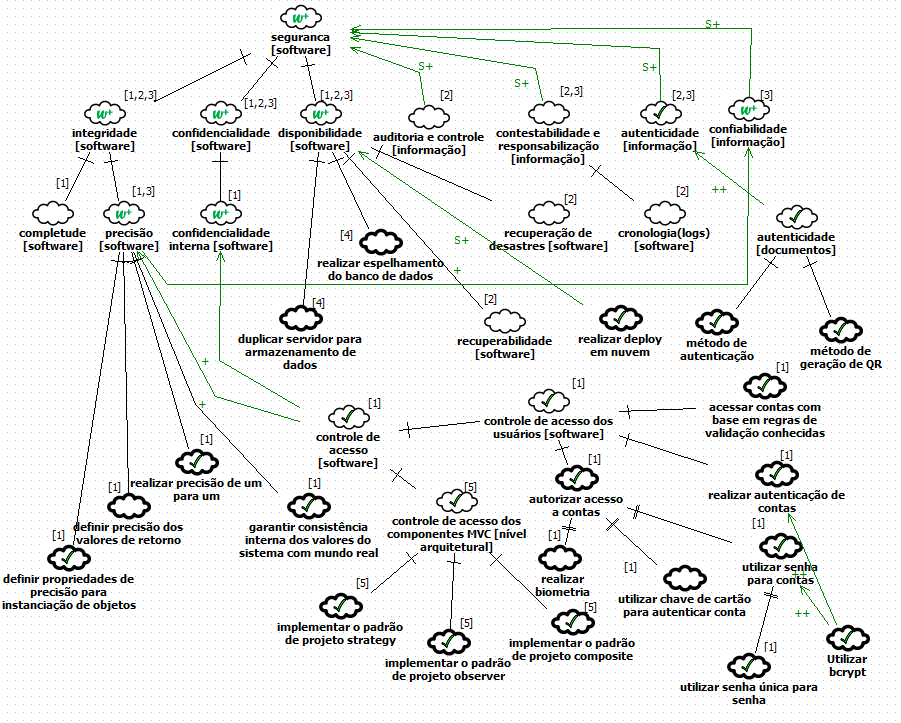
\includegraphics[keepaspectratio=true,scale=0.7]{figuras/catalogoPersona4.PNG}
	\caption{Catálogo de Segurança aplicado a sistema de geração de documentos digitais.}
	\label{catalogoPersona4}
\end{figure}

A aplicação do Catálogo de Segurança apresentado na Figura \ref{catalogoPersona4} possui uma extensão devido a utilização de assinatura digital nos documentos, que é modelada como uma meta flexível que está suficientemente satisfeita, pois depende de duas operacionalizações. As operacionalizações fazem uma relação do tipo AND com a meta flexível e ambas estão suficientemente satisfeitas, sendo elas “método de geração de (\textit{Quick Response} Quick) QR” e o  “método de autenticação” que utiliza valores como o identificador do usuário e a \textit{string} do QR. Essas relações satisfazem suficientemente a meta flexível para autenticidade da informação. 

O controle de acesso do software é satisfeito devido a relação das metas flexíveis e operacionalizações, da mesma forma que os cenários \ref{subsec:persona2} e \ref{subsec:persona1} anteriores, que já apresentaram os mesmos relacionamentos, com mesmos níveis de satisfação.  

Já a operacionalização “definir propriedades de precisão para instanciação de objetos” é escrita em cada \textit{model}, onde o \textit{Rails} permite escrever os parâmetros para controle de instanciação dos objetos. Neste cenário, foi aplicado que o atributo da classe tem que existir no banco de dados, não podendo colocar vazio ou nulo. 

A aplicação está em um servidor da Google, na nuvem, garantindo sua disponibilidade e satisfazendo então, suficientemente a operacionalização “realizar deploy em nuvem”. 

Semelhante as aplicações dos cenários \ref{subsec:persona2} e \ref{subsec:persona3} a “precisão de um para um” é suficientemente satisfeita. 

\section{Cenário 5}
\label{subsec:persona5}

Chung, 40 anos, Engenheiro de Software possui em seu quadro de responsabilidades a função de realizar manutenção e evolução de um dos sistemas pelo qual é responsável. Desse modo, percebeu que um de seus sistemas poderia ficar indisponível caso ocorresse algum problema no servidor de banco de dados. Preocupado com a segurança de seus sistemas, utilizou o Catálogo de Segurança para analisar o impacto que o espelhamento da base de dados causaria na segurança do software como um todo. 

\subsection{Aplicação do Catálogo de Segurança}

\begin{figure}[h!]
	\centering
	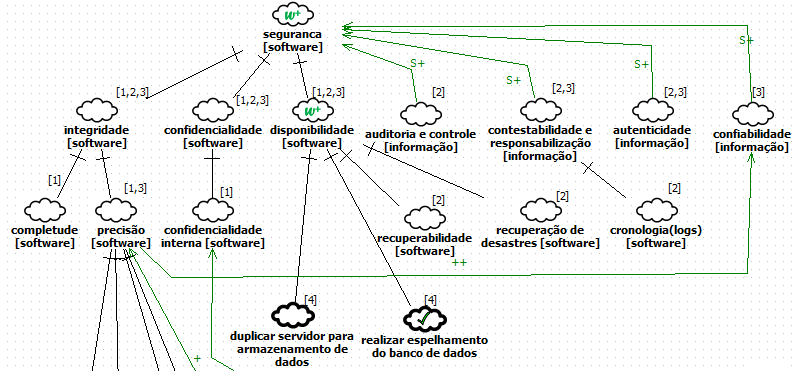
\includegraphics[keepaspectratio=true,scale=0.7]{figuras/catalogoPersona5.PNG}
	\caption{Catálogo de Segurança com foco em disponibilidade aplicado ao contexto de duplicação de base de dados.}
	\label{catalogoPersona5}
\end{figure}

A operacionalização “espelhamento da base de dados” é suficientemente satisfeita, satisfazendo parcialmente a disponibilidade do software. Esse cenário, em especial, foi modelado justamente para demonstrar o impacto de ações realizadas na base de dados na segurança do software, como apresentado na Figura \ref{catalogoPersona5}.


\section{Primeira visão do Catálogo de Segurança após as aplicações nos cenários}
\label{sec:aplicacaoDoCatalogo}

Ao modelar o Catálogo de Segurança pela primeira vez sem ter realizado nenhuma interação com algum tipo de cenário, obteve-se visão preliminar sobre Segurança devido à subjetividade e ao conjunto de conceitos abstratos presentes na literatura.  

Ao demonstrar a aplicação do Catálogo de Segurança nos cenários, observou-se que o mesmo permite, não somente a visão preliminar da segurança de software, mas também de segurança da informação.

Como o Catálogo de Segurança foi aplicado em cenários onde a ferramenta de apoio ao desenvolvimento era o \textit{Rails}, foi possível abstraí-lo para aplicações em \textit{Rails}, demonstrando então, a adaptabilidade do mesmo, como pode ser visualizado na Figura \ref{catalogoFull}.

\begin{figure}[h!]
	\centering
	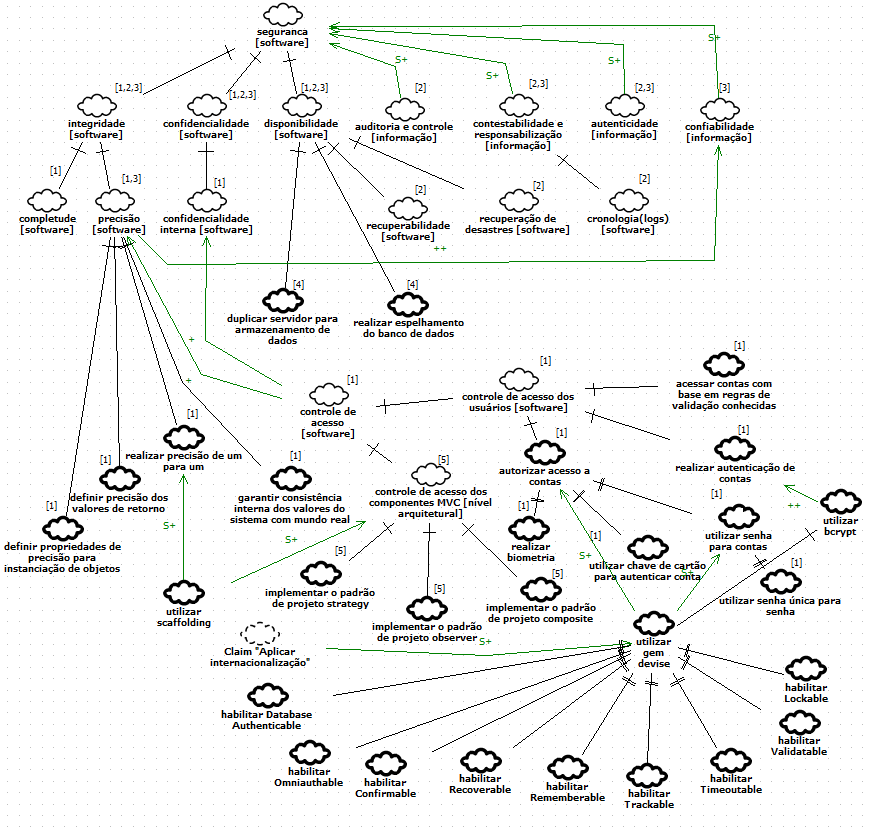
\includegraphics[keepaspectratio=true,scale=0.65]{figuras/catalogoFull.PNG}
	\caption{Versão extendida do catálogo focada em projetos \textit{rails}}
	\label{catalogoFull}
\end{figure}


Entretanto, durante a validação do Catálogo de Segurança, foram utilizados projetos em cenários reais e abstrações de possíveis usuários e cenários, tornando-o mais abrangente, caso a tecnologia utilizada seja o \textit{Rails}. Como um exemplo de evolução do Catálogo de Segurança e as evidências comprovadas da relação entre as operacionalizações e as camadas do Padrão Arquitetural MVC, é possível unificar com fins de demonstração o Catálogo de Segurança com um diagrama de componentes do padrão MVC, onde as operacionalizações estão dentro do componente ao qual possui relacionamento, como pode ser visualizado na Figura \ref{catalogoMapeado}. 


\begin{comment}
	A Tabela \ref{resultadosObtidos} apresenta de acordo com os objetivos específicos do trabalho, usando "atendido", "parcialmente atendido" e "não atendido", os principais resultados obtidos até o momento, com a realização do TCC1.	
\end{comment}

\begin{figure}[h!]
	\centering
	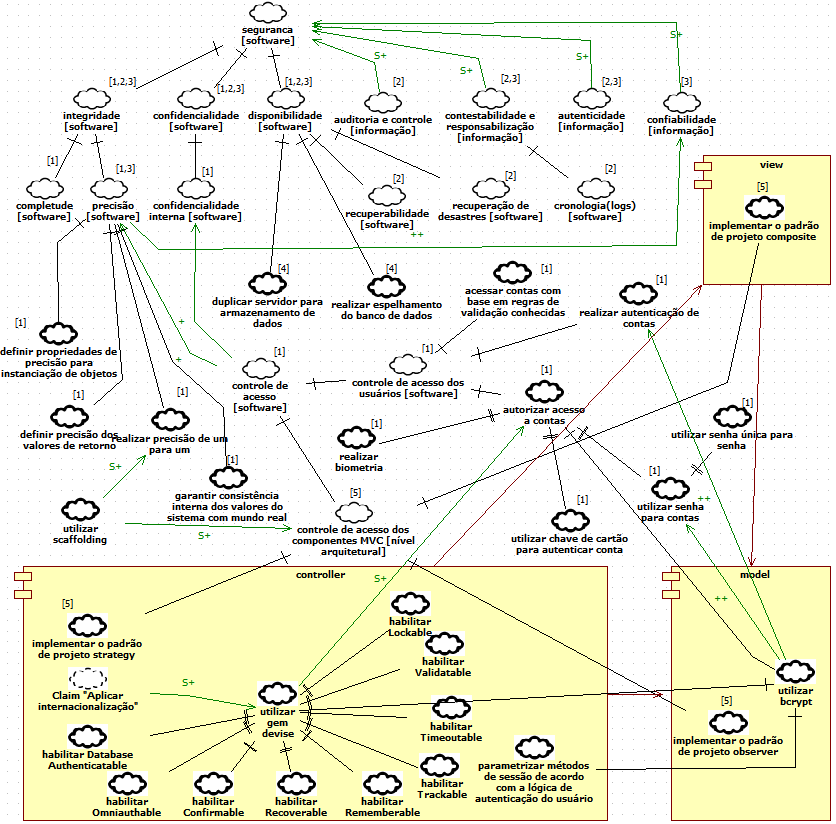
\includegraphics[keepaspectratio=true,scale=0.7]{figuras/catalogoMapeado.PNG}
	\caption{Mapeamento das metas flexíveis e operacionalizações com as camadas do MVC.}
	\label{catalogoMapeado}
\end{figure}

\section{Resumo do Capítulo}

Neste capítulo, foram apresentadas as primeiras aplicações do Catálogo de Segurança, realizadas através de cinco cenários, onde foi possível demonstrar a aplicabilidade e a adaptabilidade do Catálogo de Segurança, de acordo com o contexto. A partir da seção \ref{sec:aplicacaoDoCatalogo}, foi possível evidenciar a evolução do Catálogo de Segurança para as aplicações em projetos em \textit{Rails} e, por fim, o mapeamento em terceiro nível de abstração, sendo possível identificar as operacionalizações relacionadas com as camadas do Padrão Arquitetural MVC para projetos em \textit{Rails}.

\begin{comment}
	\begin{table}[h!]
	\centering
	\caption{Resultados obtidos de acordo com os objetivos específicos.}
	\label{resultadosObtidos}
	\tiny
	\begin{tabular}{@{}p{6cm}p{3cm}p{6cm}@{}}
	\toprule
	\textbf{Objetivo} & \textbf{Nível de satisfação} & \textbf{Motivo} \\ \midrule
	Investigar na literatura formas de lidar com o RNF Segurança  em aplicações Web desenvolvidas utilizando o MVC. & Parcialmente atendido & Parcialmente atendido, pois existem fontes não confiáveis que comprovam o impacto do RNF Segurança com aplicações web desenvolvidas utilizando o MVC, um exemplo claro de fonte não confiável são os fóruns de dúvidas. Considera-se que ao desenvolver a aplicação fica mais evidente e possível comprovar as formas de lidar com o RNF segurança no Padrão arquitetural MVC. \\
	\rowcolor[HTML]{C0C0C0} 
	Investigar na literatura os RNF associados a segurança e identificar o impacto e as interdepêndencias entre eles. & Parcialmente atendido & Parcialmente atendido, pois a subjetividade dos RNFs para Segurança dificulta o tratamento, além de dificultar a identificação do impacto entre eles. \\
	Elaborar SIG & Atendido & Atendido, pois tem-se a primeira versão do catálogo elaborado com sucesso. \\
	\rowcolor[HTML]{C0C0C0} 
	Realizar correspondência entre o catálogo e as camadas do padrão arquitetural MVC & Atendido & Atendido, pois essa correspondência foi analisada de acordo com a base teórica já levantada. \\ \bottomrule
	\end{tabular}
	\end{table}
\end{comment}


\chapter{Conclusão}
\label{chap:consideracoesFinais}



Dada a complexidade do tema, em especial por procurar contribuir partindo de critérios de qualidade que são intrinsecamente abstratos e subjetivos, sabe-se que o Catálogo de Segurança ainda reflete uma visão preliminar sobre Segurança. Portanto, com o Catálogo de Segurança espera-se que a contribuição evidenciada neste trabalho possa ser atendida e aplicada dentro dos vários cenários da Engenharia de Software (Ex: Arquitetura e Desenho de Software, Engenharia de Requisitos e Desenvolvimento de Software), visto que uma vez que vislumbra uma forma de trabalhar critérios tão abstratos (os requisitos não funcionais ou metas flexíveis e suas dependências e seus impactos), trazendo-os para uma visão bem mais concreta, as operacionalizações. Tudo garantido com o uso de uma notação bastante rica e emergente, a qual é muito mais conhecida e compreendida na subárea de Engenharia de Requisitos. Esse trabalho aproximou esses conhecimentos, considerando níveis de abstração cada vez mais técnicos. Assim, ao decorrer do trabalho foram apresentados detalhamentos que deixam evidentes as correlações entre esses níveis de abstração, Requisitos Não-Funcionais e Código, os quais parecem distantes. Essa distância comumente reflete em esquecimento, ou seja, não atendimento desses critérios de qualidade no desenvolvimento do software desejado. Prática essa que pode levar a muitos insucessos em projetos de software. 

Portanto o Catálogo de Segurança, pode ser relacionado com outros catálogos voltados aos atributos de qualidade (Ex: usabilidade, desempenho, etc.) e que utilizam a mesma notação, permitindo realizar o mapeamento, verificar o impacto que as outras áreas de qualidade de software impactam a Segurança do mesmo. O Catálogo de Segurança apresentado neste trabalho também pode evoluir a níveis cada vez mais baixos de abstração, podendo entrar em questão, por exemplo, qual método de criptografia pode ser mais eficiente para uma determinada operacionalização?, ou até mesmo ser expandido para questões como segurança da informação.  


\begin{comment}
	Prática essa que pode levar a muitos insucessos, tais como o Caso da Ambulância de Londres \cite{finkelstein1996comedy}.
\end{comment}
 


\begin{comment}


	
	
	Esse Capítulo procura apresentar um resumo quanto aos resultados alcançados até o momento, com a realização do presente trabalho, bem como o que ainda será alcançado com a realização do TCC2. Dessa forma, a seção \ref{sec:resultadosObtidos} procura resgatar os objetivos geral e específicos apresentados no Capítulo \ref{chap:introducao}, detalhando em uma tabela (ou em um quadro) o que foi atendido em tempo de TCC1. Na seção \ref{sec:resultadosEsperados}, outra tabela (ou outro quadro) é apresentada(o), procurando acordar o que ainda será atendido em tempo de TCC2.
	
	\section{Resultados Esperados}
	\label{sec:resultadosEsperados}
	
	É muito provável em tempo de execução do TCC2 o nível de mapeamento entre as metas flexíveis e o  Padrão Arquitetural MVC possa ser refinado. Acredita-se que ao desenvolver o software utilizando o Padrão arquitetural MVC, será possível compreender mais facilmente as relações entre as metas flexíveis e as operacionalizações com o padrão. 
	
	
	\begin{table}[h!]
	\centering
	\caption{Resultados esperados de acordo com os objetivos específicos.}
	\label{resultadosEsperados}
	\tiny
	\begin{tabular}{@{}p{8cm}p{7.5cm}@{}}
	\toprule
	\textbf{Objetivo} & \textbf{Resultado esperado} \\ \midrule
	Investigar na literatura formas de lidar com o RNF Segurança,em aplicações Web desenvolvidas utilizando o MVC. & Espera-se com a implementação do software validar as formas de lidar com o RNF de Segurança. \\
	\rowcolor[HTML]{C0C0C0} 
	Investigar na literatura os RNF associados a segurança e identificar o impacto e as interdepêndencias entre eles. & Espera-se com a implementação do software identificar os impactos e as interdepêndencias com os RNFs de Segurança de acordo com as metas flexiveis a serem definidas de acordo com o contexto em que o software será desenvolvido. \\
	Desenvolver aplicação web utilizando o Padrão Arquitetural MVC & Através do desenvolvimento da aplicação realizar a coleta das primeiras impressões da aplicação do catálogo, evoluir o catálogo e identificar novas metas flexíveis e operacionalizações para evoluir o catálogo. \\ \bottomrule
	\end{tabular}
	\end{table}
	
	\section{Resumo do Capítulo}
	
	Acredita-se que o principal intuito dessa pesquisa esteja sendo alcançado, uma vez que o catálogo de Segurança pode ser visto como um exemplo de como aproximar a especificação de algo tão abstrato, como são os RNFs ou critérios de qualidade, de insumos mais concretos - operacionalizações, os quais podem ser mais bem compreendidos bem como mais úteis aos membros da equipe de desenvolvimento. Lembrando que esses membros atuam em atividades que se encontram em níveis mais baixos de abstração - ou seja, mais próximos de código. A intenção é ajudá-los no cumprimento dessas especificações de requisitos não-funcionais, comumente negligenciados \cite{eckhardt2016non}.
	
\end{comment}


\chapter[Elementos do Texto]{Elementos do Texto}

\section{Corpo do Texto}

O estilo de redação deve atentar a boa prática da linguagem técnica. Para a 
terminologia metrological usar o Vocabulário Internacional de Termos 
Fundamentais e Gerais de Metrologia \cite{inmetro2003}.

Grandezas dimensionais devem ser apresentadas em unidades consistentes com 
o Sistema Internacional de Unidades  (SI). Outras unidades podem ser usadas 
como unidades secundárias entre parenteses se necessário. Exceções são 
relacionadas a unidades não-SI usadas como identificadores comerciais como 
pro exemplo \lq\lq disquete de  3$\nicefrac{1}{2}$ polegadas\rq\rq. 

Na apresentação de números ao longo do texto usar virgula para separar a 
parte decimal de um número. Resultados experimentais devem ser apresentados 
com sua respectiva incerteza de medição.

\section{Títulos de capítulos e seções}

Recomendações de formatação de seções (texto informativo: o \LaTeX\
\textbf{já formata as seções automaticamente, se utilizado o comando
\texttt{\textbackslash section\{Nome da Seção\}}}):

\begin{description}

	\item \textbf{1 SEÇÃO PRIMÁRIA - MAIÚSCULAS; NEGRITO; TAMANHO 12;}

	\item 1.1 SEÇÃO SECUNDÁRIA – MAIÚSCULAS; NORMAL; TAMANHO 12; 

	\item \textbf{1.1.1 Seção terciária - Minúsculas, com exceção da 
	primeira letra; negrito; tamanho 12;}

	\item 1.1.1.1 Seção quaternária - Minúsculas, com exceção da primeira 
	letra; normal tamanho 12; 

 	\item \textit{1.1.1.1.1 Seção quinária - Minúsculas, com exceção da 
	primeira letra; itálico; tamanho 12.}

\end{description}

\section{Notas de rodapé}

Notas eventualmente necessárias devem ser numeradas de forma seqüencial ao 
longo do texto no formato 1, 2, 3... sendo posicionadas no rodapé de cada 
página na qual a nota é utilizada.\footnote{Como, por exemplo, esta nota. O \LaTeX\ tomará conta da numeração automaticamente.}

\section{Equações}

Equações matemáticas devem ser numeradas seqüencialmente e alinhadas a 
esquerda com recuo de 0,6 cm. Usar numerais arábicos entre parênteses, 
alinhado a direita, no formato Times New Roman de 9 pts. para numerara as 
equações como mostrado na Eq. \ref{eqn01} (novamente, o \LaTeX\ formata as
equações automaticamente).

Referências a equações no corpo do texto devem ser feitas como \lq\lq Eq. 
\ref{eqn01}\rq\rq\ quando no meio de uma frase ou como \lq\lq Equação 
\ref{eqn01}\rq\rq\ quando no inicio de uma sentença. Um espaçamento de 11 
pontos deve ser deixado acima, abaixo e entre equações subseqüentes. Para uma 
apresentação compacta das equações deve-se usar os símbolos e expressões 
matemáticos mais adequados e parênteses para evitar ambigüidades em 
denominadores. Os símbolos usados nas equações citados no texto devem 
apresentar exatamente a mesma formatação usada nas equações.
\begin{equation}
\label{eqn01}
	\frac{d\mathbf{C}}{dw} = \frac{du}{dw}\cdot \mathbf{F}_u + 
		\frac{dv}{dw}\cdot \mathbf{F}_v 
\end{equation}

O significado de todos os símbolos mostrados nas equações deve ser apresentado 
na lista de símbolos no inicio do trabalho, embora, em certas circunstancias o 
autor possa para maior clareza descrever o significado de certos símbolos no 
corpo do texto, logo após a equação.

Se uma equação aparecer no meio do parágrafo, como esta
\begin{equation}
x^n + y^n = z^n,
\end{equation}
onde $x, y, z, n \in \mathbf{N}$, o texto subsequente faz parte do parágrafo e 
não deve ser identado.

\section{Figuras e Gráficos}

As figuras devem ser centradas entre margens e identificadas por uma legenda 
alinhada a esquerda com recuo especial de deslocamento de 1,8 cm, com mostrado 
na Fig. (\ref{fig01}). O tamanho das fontes empregadas nos rótulos e anotações 
usadas nas figuras deve ser compatível com o usado no corpo do texto. Rótulos e 
anotações devem estar em português, com todas as grandezas mostradas em 
unidades do SI (Sistema Internacional de unidades) (mais uma vez, o \LaTeX\
cuidará dos aspectos de formatação e fonte das figuras).

Todas as figuras, gráficos e fotografias devem ser numeradas e referidas no 
corpo do texto adotando uma numeração seqüencial de identificação. As figuras e 
gráficos devem ser claras e com qualidade adequada para eventual reprodução 
posterior tanto em cores quanto em preto-e-branco.

As abscissas e ordenadas de todos os gráficos devem ser rotuladas com seus 
respectivos títulos em português seguida da unidade no SI que caracteriza a 
grandes entre colchetes. 

A referência explícita no texto à uma figura deve ser feita como 
\lq\lq Fig. \ref{fig01}\rq\rq\ quando no meio de uma frase ou como 
\lq\lq Figura \ref{fig01}\rq\rq\ quando no início da mesma. Referencias 
implícitas a uma dada figura devem ser feitas entre parênteses como 
(Fig. \ref{fig01}). Para referências a mais de uma figura as mesmas regras 
devem ser aplicadas usando-se o plural adequadamente. Exemplos:

\begin{itemize}
	\item \lq\lq Após os ensaios experimentais, foram obtidos os resultados 
	mostrados na Fig. \ref{fig01}, que ...\rq\rq
	\item \lq\lq A Figura \ref{fig01} apresenta os resultados obtidos, onde 
	pode-se observar que ...\rq\rq
	\item \lq\lq As Figuras 1 a 3 apresentam os resultados obtidos, 
	...\rq\rq
	\item \lq\lq Verificou-se uma forte dependência entre as variáveis citadas 
	(Fig. \ref{fig01}), comprovando ...\rq\rq
\end{itemize}

Cada figura deve ser posicionada o mais próxima possível da primeira citação 
feita à mesma no texto, imediatamente após o parágrafo no qual é feita tal 
citação, se possível, na mesma página. Em \LaTeX\, o comando \texttt{\textbackslash label} deve suceder o comando \texttt{\textbackslash caption} para que as referências às figuras fiquem com a numeração correta.
\begin{figure}[h]
	\centering
	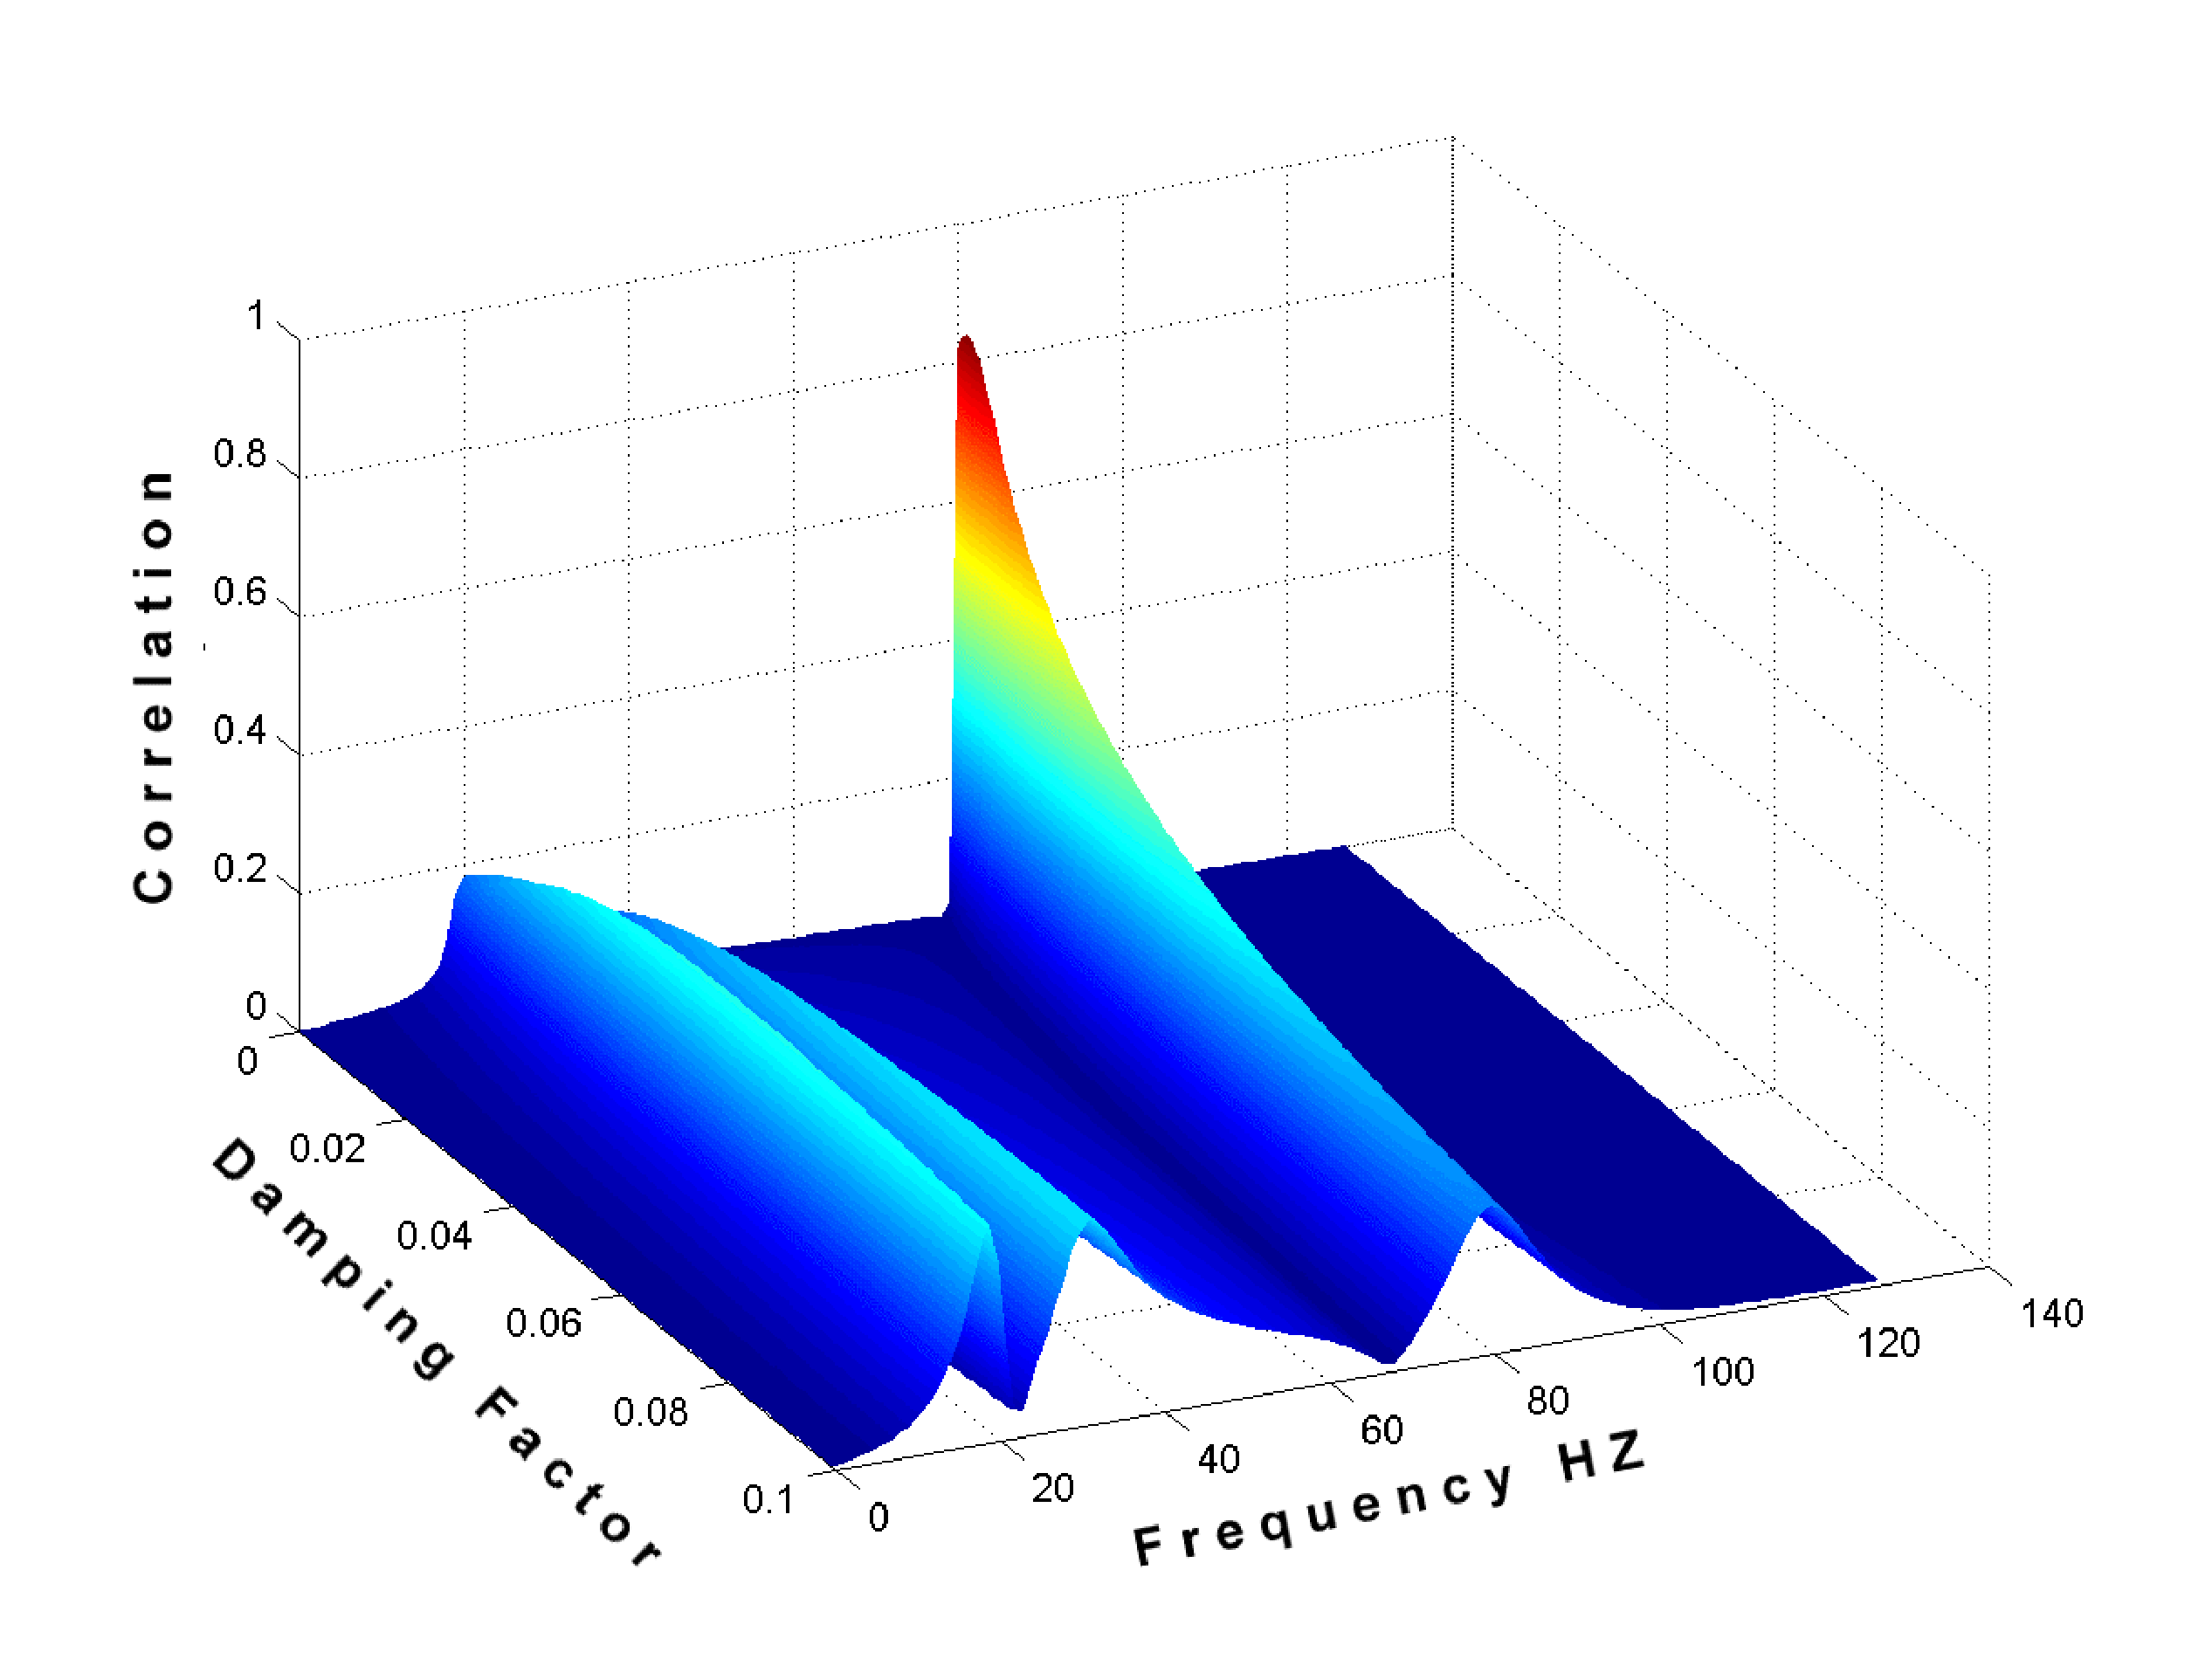
\includegraphics[keepaspectratio=true,scale=0.3]{figuras/fig01.eps}
	\caption{Wavelets correlation coefficients}
	\label{fig01}
\end{figure}

\section{Tabela}

As tabelas devem estar centradas entre margens e identificadas por uma legenda 
alinhada a esquerda, com recuo especial de deslocamento de 1,8 cm, posicionada 
acima da tabela com mostrado na Tab. \ref{tab01}, a título de 
exemplo. O tamanho das fontes empregadas nos rótulos e anotações usadas nas 
tabelas deve ser compatível com o usado no corpo do texto. Rótulos e anotações 
devem estar em português. Um espaçamento de 11 pts deve ser deixado entre a 
legenda e a tabela, bem como após a tabela. A numeração, a fonte e a formatação
são automáticas quando se usa o \LaTeX.

As grandezas dimensionais mostradas em cada tabela devem apresentar unidades 
consistentes com o SI. As unidades de cada variável devem ser mostradas apenas 
na primeira linha e/ou coluna da tabela, entre colchetes 

A referência explícita no texto à uma dada tabela deve ser feita como 
\lq\lq Tab. \ref{tab01}\rq\rq\ quando no meio de uma frase ou como 
\lq\lq Tabela \ref{tab01}\rq\rq\ quando no início da mesma. Referências 
implícitas a uma dada tabela devem ser feitas entre parênteses como 
(Tab. \ref{tab01}). Para referências a mais de uma tabela as mesmas 
regras devem ser aplicadas usando-se o plural adequadamente. Exemplos:
\begin{itemize}
	\item \lq\lq Após os ensaios experimentais, foram obtidos os resultados 
	mostrados na Tab. \ref{tab01}, que ...\rq\rq
	\item \lq\lq A Tabela \ref{tab01} apresenta os resultados obtidos, onde 
	pode-se observar que ...\rq\rq
	\item \lq\lq As Tabelas 1 a 3 apresentam os resultados obtidos, ...\rq\rq
	\item \lq\lq Verificou-se uma forte dependência entre as variáveis citadas 
	(Tab. \ref{tab01}), comprovando ...\rq\rq
\end{itemize}

Cada tabela deve ser posicionada o mais próxima possível da primeira citação 
feita à mesma no texto, imediatamente após o parágrafo no qual é feita a 
citação, se possível, na mesma página.

\begin{table}[h]
	\centering
	\caption{Propriedades obtidades após processamento}
	\label{tab01}
	
	\begin{tabular}{ccc}
		\toprule
		\textbf{Processing type} & \textbf{Property 1} (\%) & 
		\textbf{Property 2} $[\mu m]$ \\
		\midrule
		Process 1 & 40.0 & 22.7 \\
		Process 2 & 48.4 & 13.9 \\
		Process 3 & 39.0 & 22.5 \\
		Process 4 & 45.3 & 28.5 \\
		\bottomrule
	\end{tabular}
\end{table}

\section{Citação de Referências}

Referencias a outros trabalhos tais como artigos, teses, relatórios, etc. devem 
ser feitas no corpo do texto devem estar de acordo com a norma corrente ABNT 
NBR 6023:2002 (ABNT, 2000), esta ultima baseada nas normas ISO 690:1987:
\begin{itemize}
	\item \lq\lq \citeonline{bordalo1989}, mostraram que...\rq\rq

	\item \lq\lq Resultados disponíveis em \cite{coimbra1978}, \cite{clark1986} 
	e \cite{sparrow1980}, mostram que...\rq\rq
\end{itemize}

Para referências a trabalhos com até dois autores, deve-se citar o nome de 
ambos os autores, por exemplo: \lq\lq \citeonline{soviero1997}, mostraram 
que...\rq\rq






\bookmarksetup{startatroot} 

\postextual

\bibliography{bibliografia} 
%\begin{apendicesenv}

%\partapendices

%\chapter{Primeiro Apêndice}

%Texto do primeiro apêndice.

%\chapter{Segundo Apêndice}

%Texto do segundo apêndice.

%\end{apendicesenv}

\begin{anexosenv}

\partanexos

\chapter{Primeiro Anexo}

Texto do primeiro anexo.

\chapter{Segundo Anexo}

Texto do segundo anexo.

\end{anexosenv}


\printindex

\end{document}

